\documentclass[xcolor=dvipsnames, 12pt]{beamer}

\usepackage{xcolor}
\usepackage{hyperref}
\usepackage[natbib=true,style=authortitle,citestyle=numeric,backend=bibtex,useprefix=true]{biblatex}
\addbibresource{refs.bib}
\usepackage[english]{babel}
\usepackage{subcaption}
\usepackage{anyfontsize}
\usepackage{t1enc}
\usepackage{booktabs}
\usepackage[font=tiny,skip=0.5pt]{caption}
\captionsetup[figure]{font=tiny,skip=0pt}
\setlength\abovecaptionskip{-5pt}
\usepackage{listings}
\usepackage{subcaption}
\usepackage{emoji}


\setlength {\marginparwidth }{2cm}

\usetheme{Madrid}

\definecolor{cnitblue}{RGB}{0, 0, 139}
%\definecolor{pblack}{RGB}{0, 0, 0}
%\definecolor{pgrey}{RGB}{127, 127, 127}

%\usepackage{soul}

\newcommand{\best}[1]{\color{cnitblue}{\underline{#1}}}

\usecolortheme[named=cnitblue]{structure}
%\setbeamercolor{item projected}{bg=pblack}
%\setbeamercolor{subitem projected}{bg=pgrey}

\title[linux day 2025]{Can an eVape say "Hello World!"?}
\subtitle{By Alessandro Rivitti \& Pierciro Caliandro}
\author[AR,PC]{Alessandro Rivitti, Caliandro Pierciro}

\institute[CNIT]{CNIT Nam Lab, Rome}
\date{\today}


\hypersetup{
    colorlinks=true,
    linkcolor=blue,
    filecolor=magenta,
    urlcolor=cyan,
}

\logo{
\includegraphics[height=0.5cm]{assets/logo.png}}
\addtobeamertemplate{navigation symbols}{}{%
    \usebeamerfont{footline}%
    \usebeamercolor[fg]{footline}%
    \hspace{1em}%
    \insertframenumber/\inserttotalframenumber
}

\setbeamertemplate{section page}{\begingroup\centering\begin{beamercolorbox}[sep=12pt,center,colsep=-4bp,rounded=true,shadow=true]{section title}\usebeamerfont{section title}\insertsection\par\end{beamercolorbox}\endgroup}

\begin{document}
	
	\begin{NoHyper}
        \frame{\titlepage}
	\end{NoHyper}

   \begin{NoHyper}
			\section{Atto 0}
			\frame{\sectionpage}
	\end{NoHyper}
        
	\begin{NoHyper}
        \begin{frame}{How it started}
			What I saw some weeks before...
			\begin{figure}
				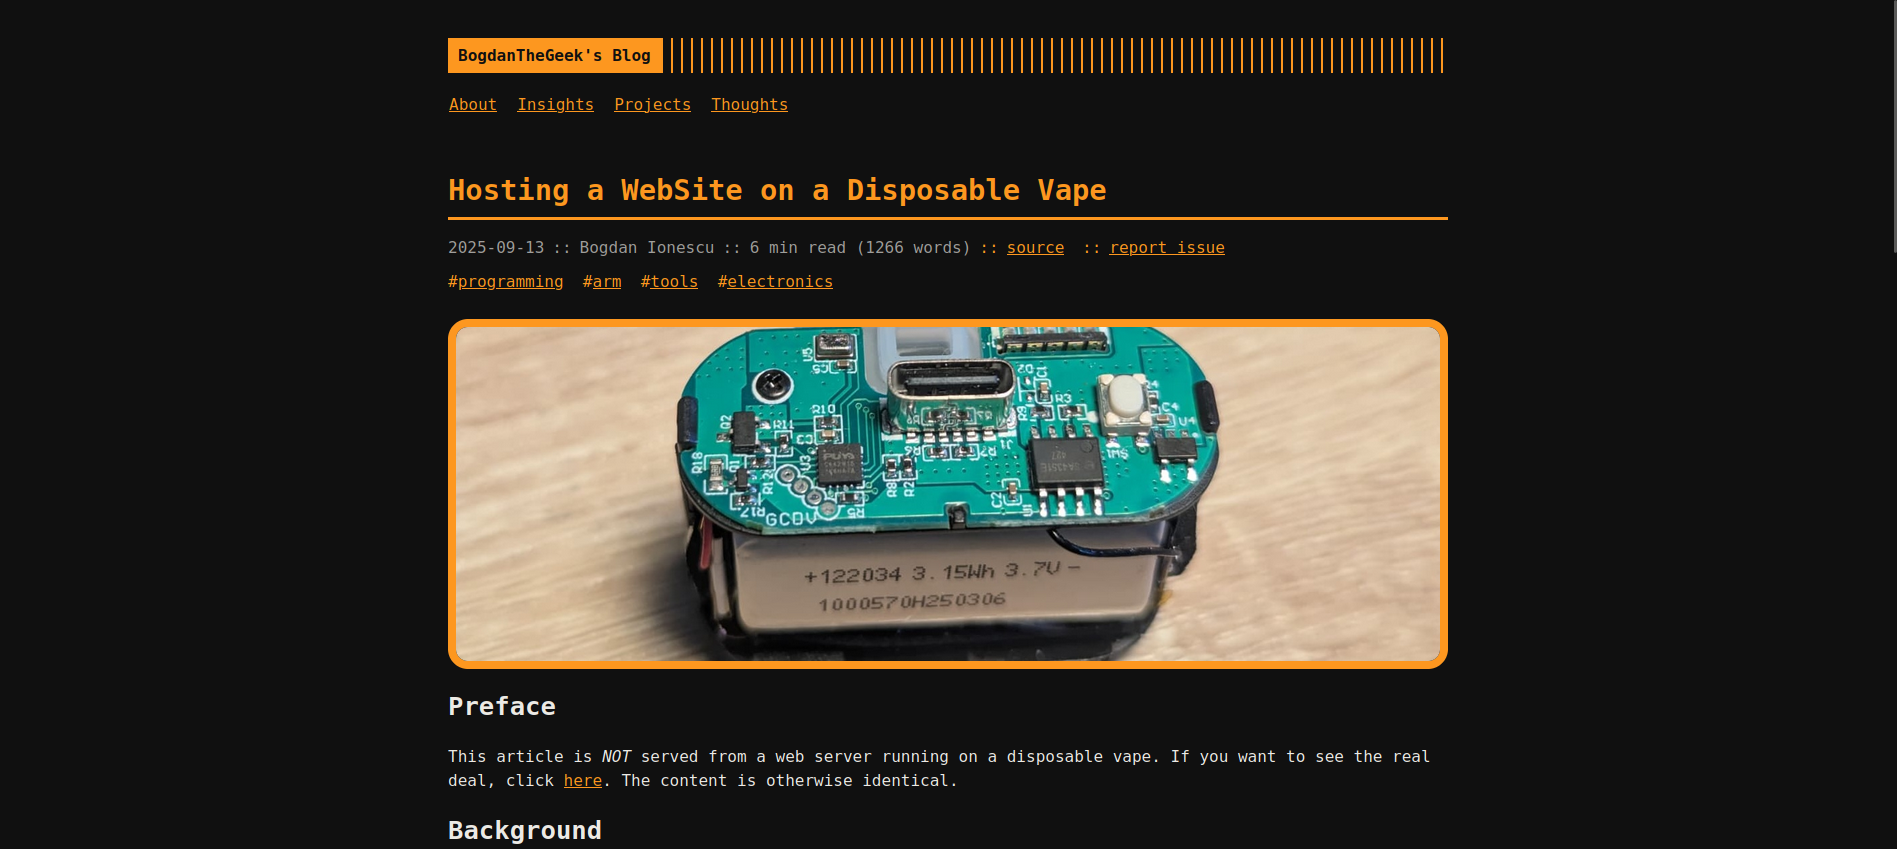
\includegraphics[width=\textwidth]{assets/blog_post.png}
			\end{figure}
			Wow! Let's try to do something similar
        \end{frame}
	\end{NoHyper}

	\begin{NoHyper}
        \begin{frame}{The problems}
			\begin{itemize}
				\item No knowledge of semihosting at all
				\item No knowledge of hardware or electronics at all
				\item I had $\approx$ 1 week to complete it...
			\end{itemize}
		\end{frame}
	\end{NoHyper}

	\begin{NoHyper}
        \begin{frame}{Problem 1 - Solution}
			There are a lot of resources online to learn about semihosting!
		\begin{minipage}[b]{.5\textwidth}
			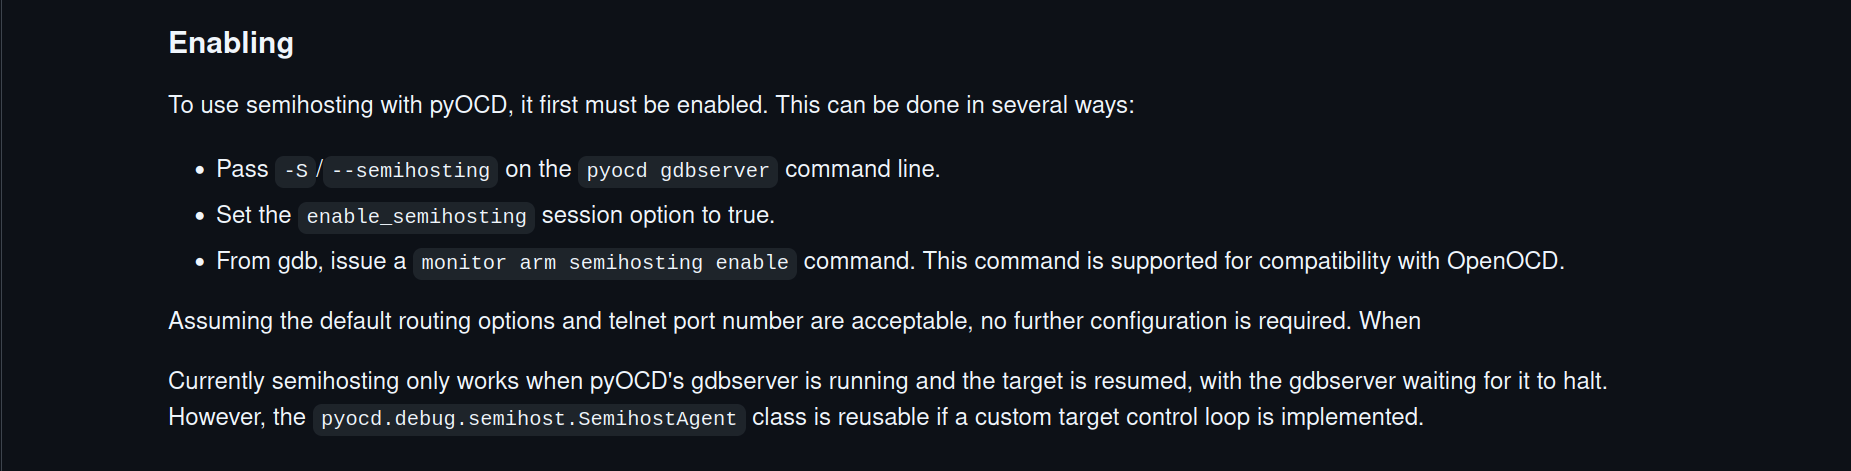
\includegraphics[width=\textwidth]{assets/semihost_1}
			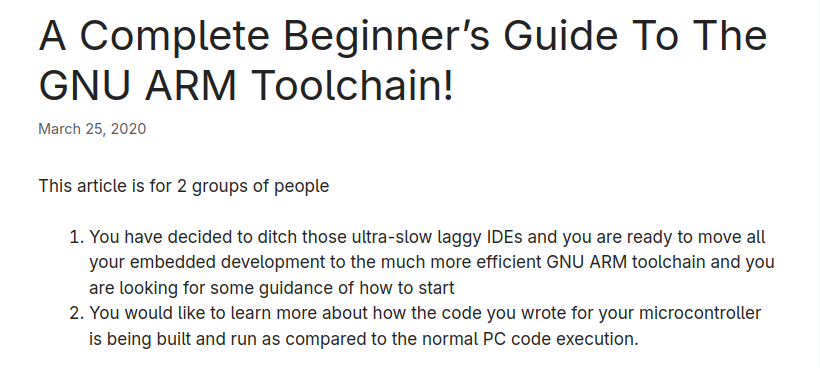
\includegraphics[width=\textwidth]{assets/semihost_3}
		\end{minipage}%
		\begin{minipage}[b]{.5\textwidth}
			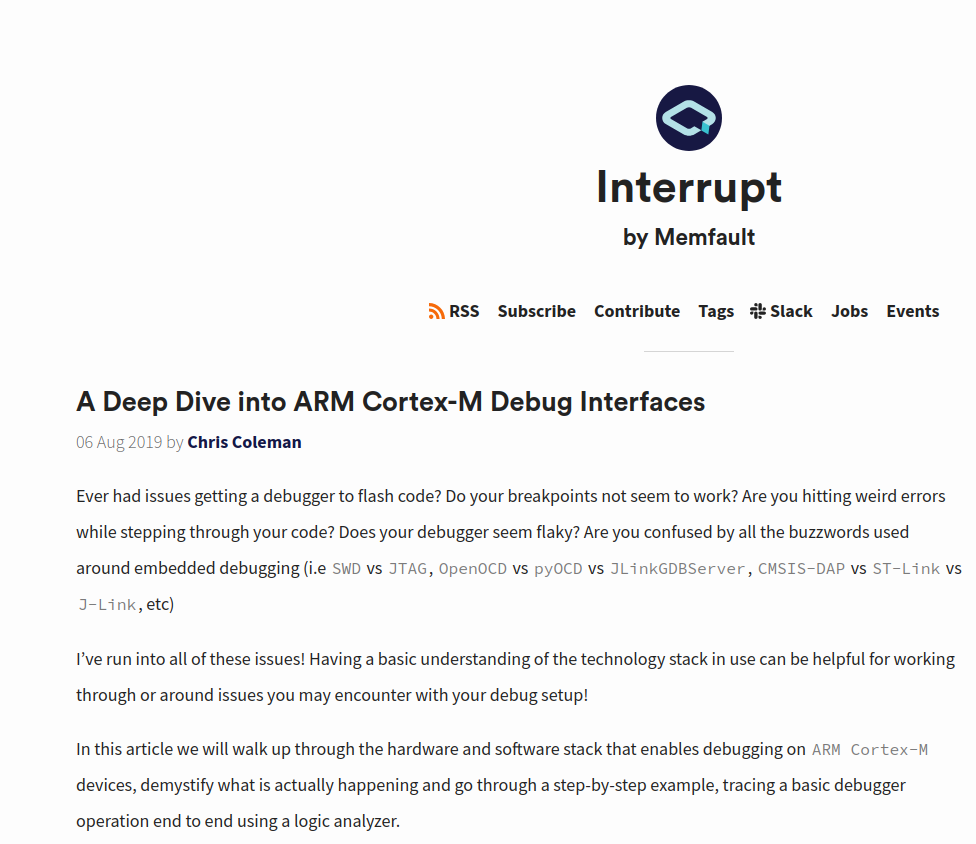
\includegraphics[width=\textwidth]{assets/semihost_2}
		\end{minipage}%
		\end{frame}
	\end{NoHyper}

	\begin{NoHyper}
        \begin{frame}{Problem 2 - Solution}	
			\begin{figure}
				\includegraphics[width=.8\textwidth]{assets/day_0.pdf}
			\end{figure}
		\end{frame}
	\end{NoHyper}

	\begin{NoHyper}
        \begin{frame}{Problem 3 - Solution}
			Let's ask to some friends if they can ""lend"" us a disposed eVape
			\begin{figure}[t!]
				\subfloat{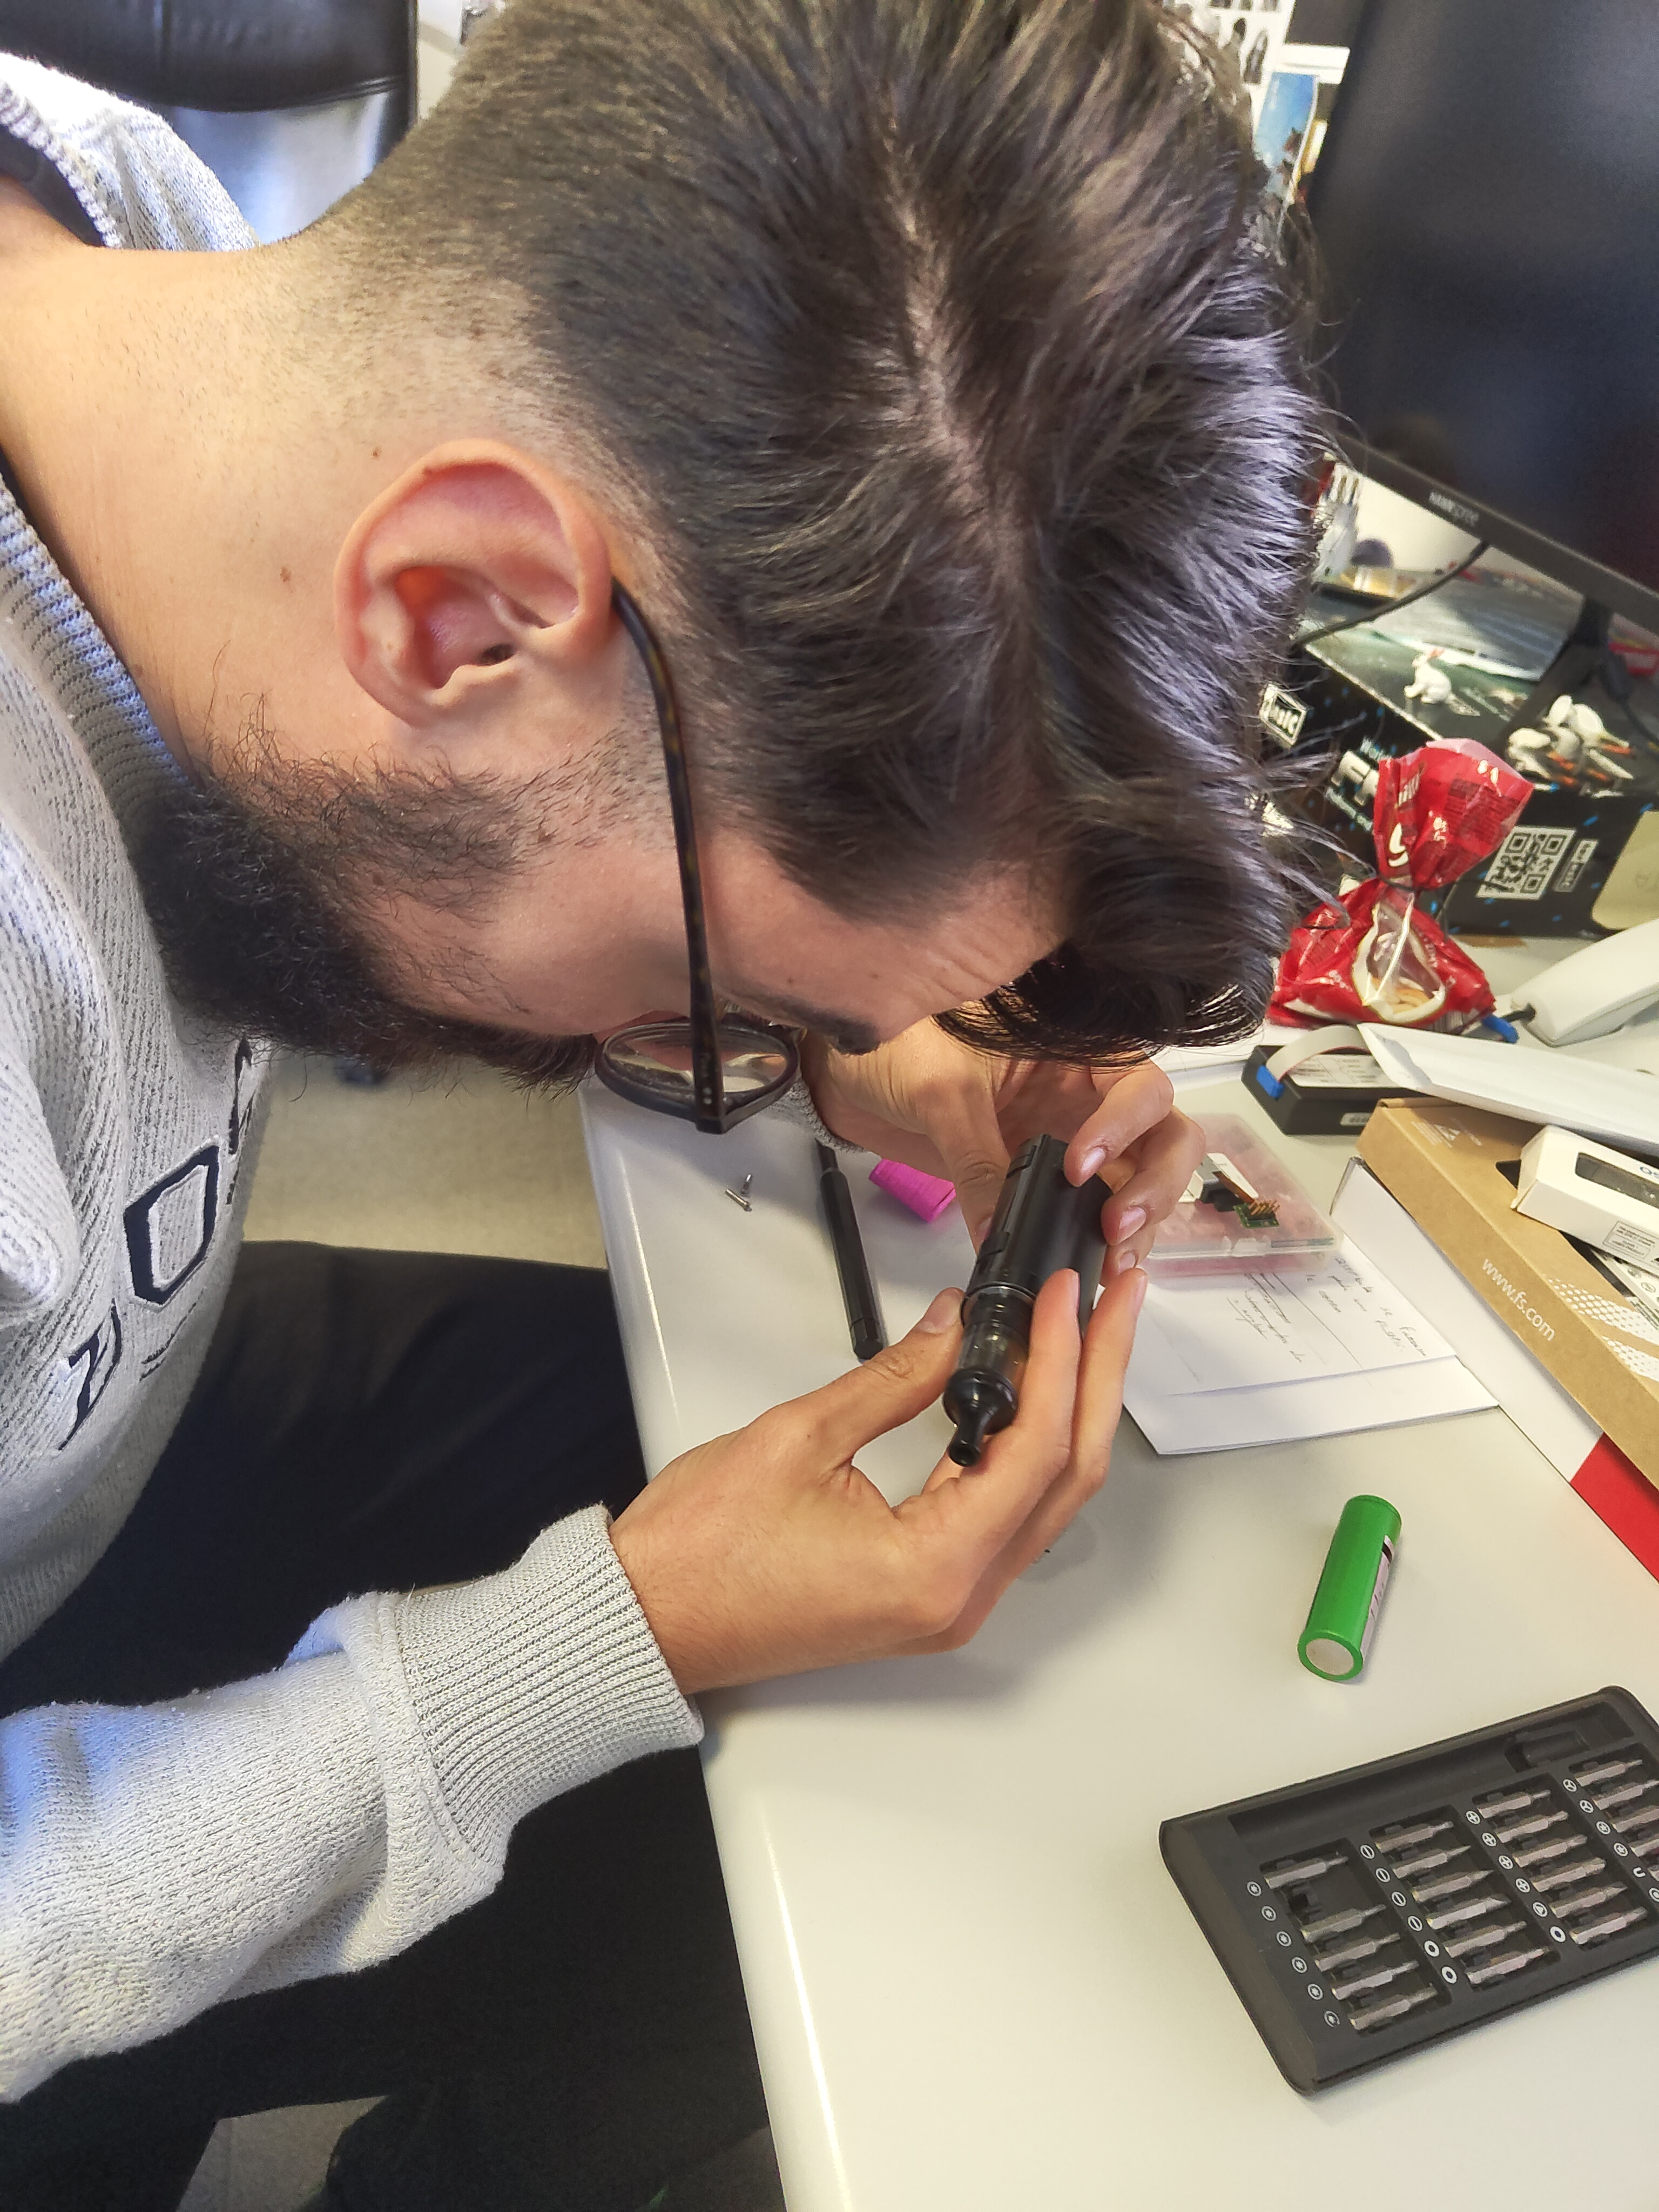
\includegraphics[width=0.3\linewidth]{assets/sigaretta_1_1.png}}\hfill
  				\subfloat{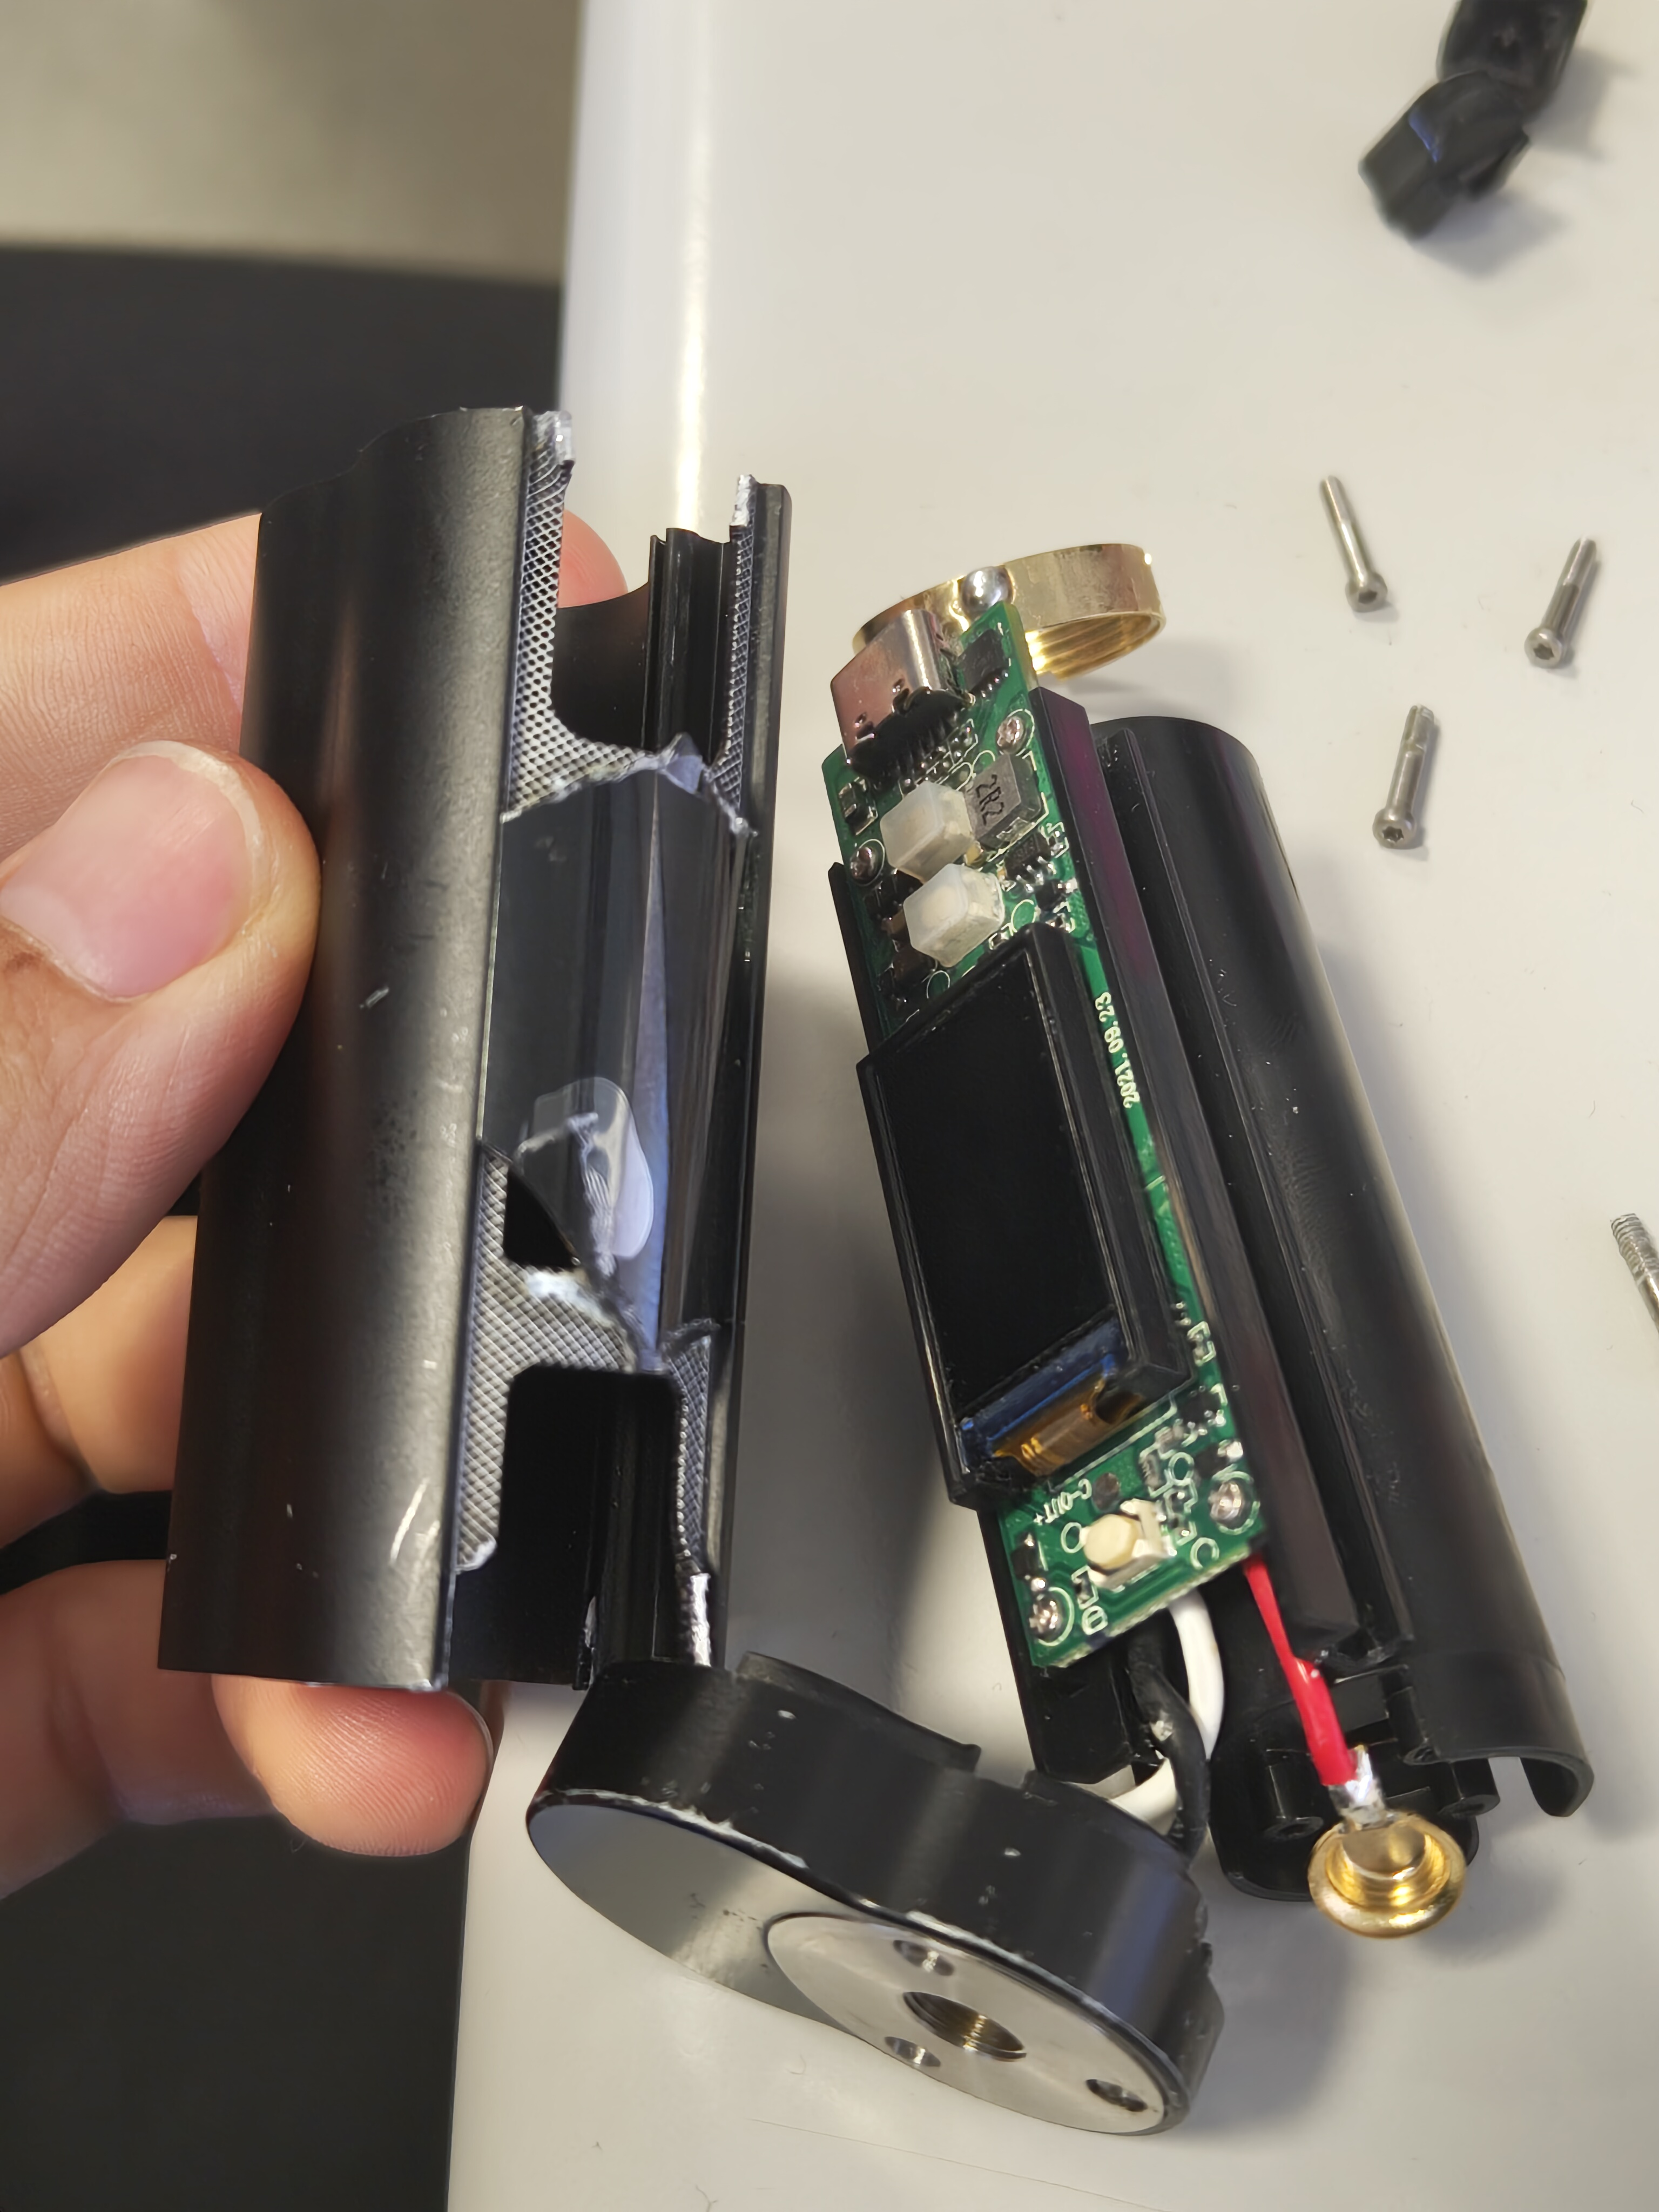
\includegraphics[width=0.3\linewidth]{assets/sigaretta_1_2.jpg}}\hfill
  				\subfloat{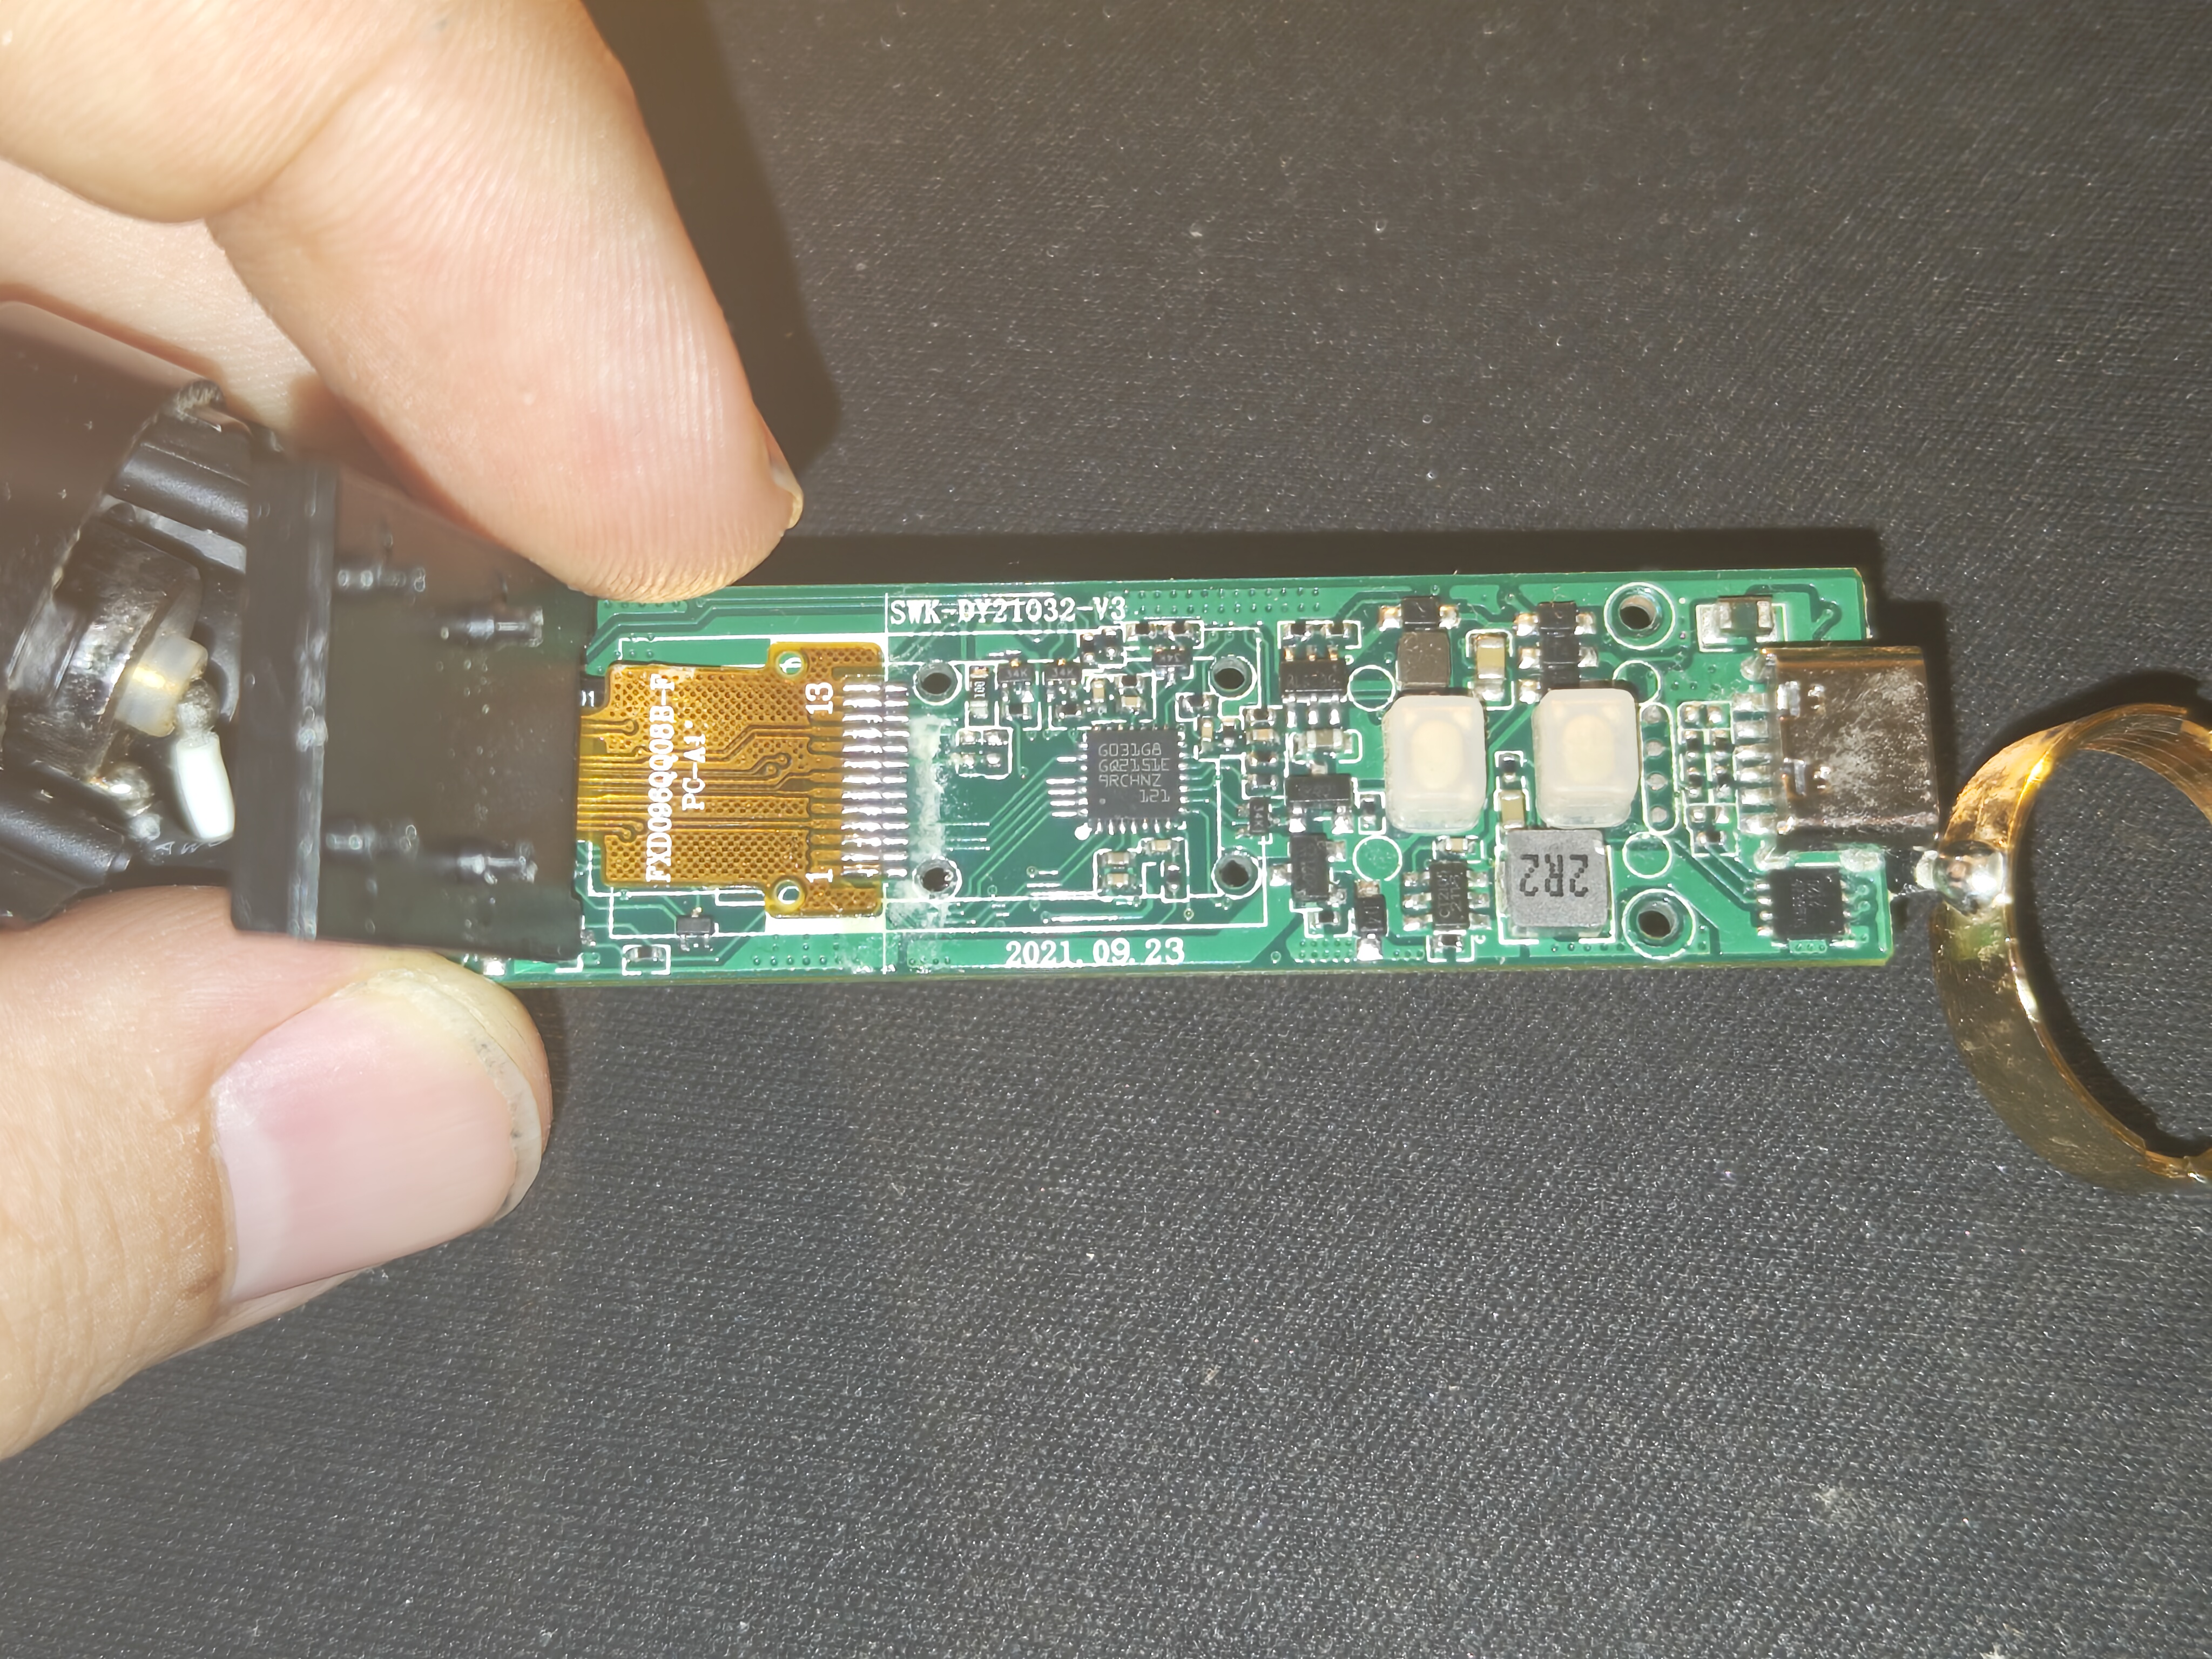
\includegraphics[width=0.35\linewidth]{assets/sigaretta_1_3.jpg}}\hfill%
			\end{figure}
		\end{frame}
	\end{NoHyper}

	\begin{NoHyper}
        \begin{frame}{Problem 3 - Problem}
			\begin{itemize}
				\item The chipset was not what we were expecting
				\item Other blog post talk about PUYA chipset
				\item We needed a "cheaper" eCig, so we needed to find another target
				\item (so sorry Angelo for breaking for cig <3)
			\end{itemize}
		\end{frame}
	\end{NoHyper}

	\begin{NoHyper}
        \begin{frame}{Problem 3 - Bogdan comes to help}
			\begin{figure}[t!]
				\subfloat{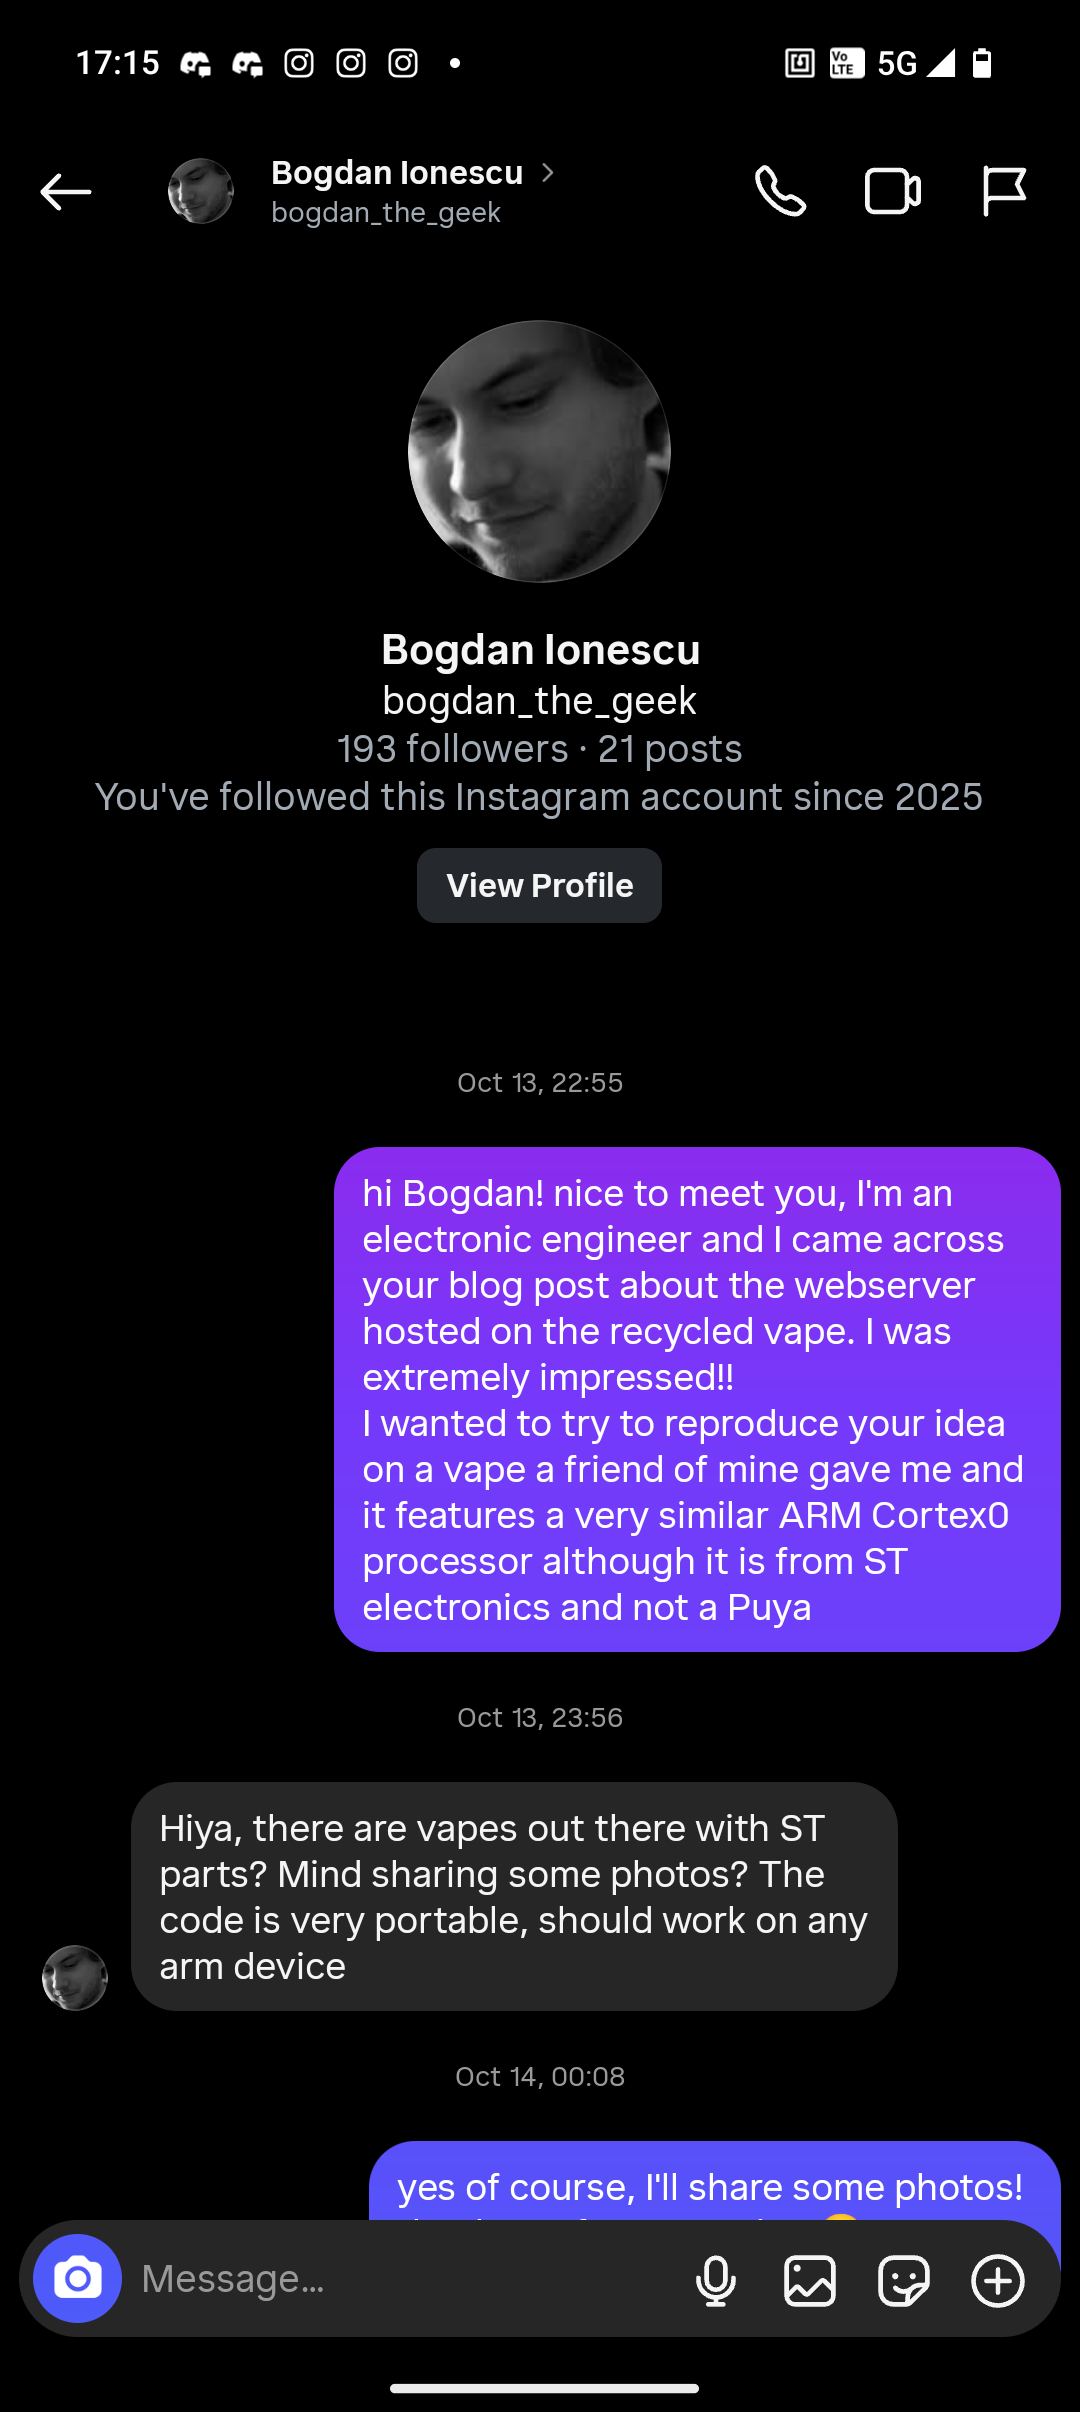
\includegraphics[width=0.3\linewidth]{assets/bogdan_1}}\hfill
  				\subfloat{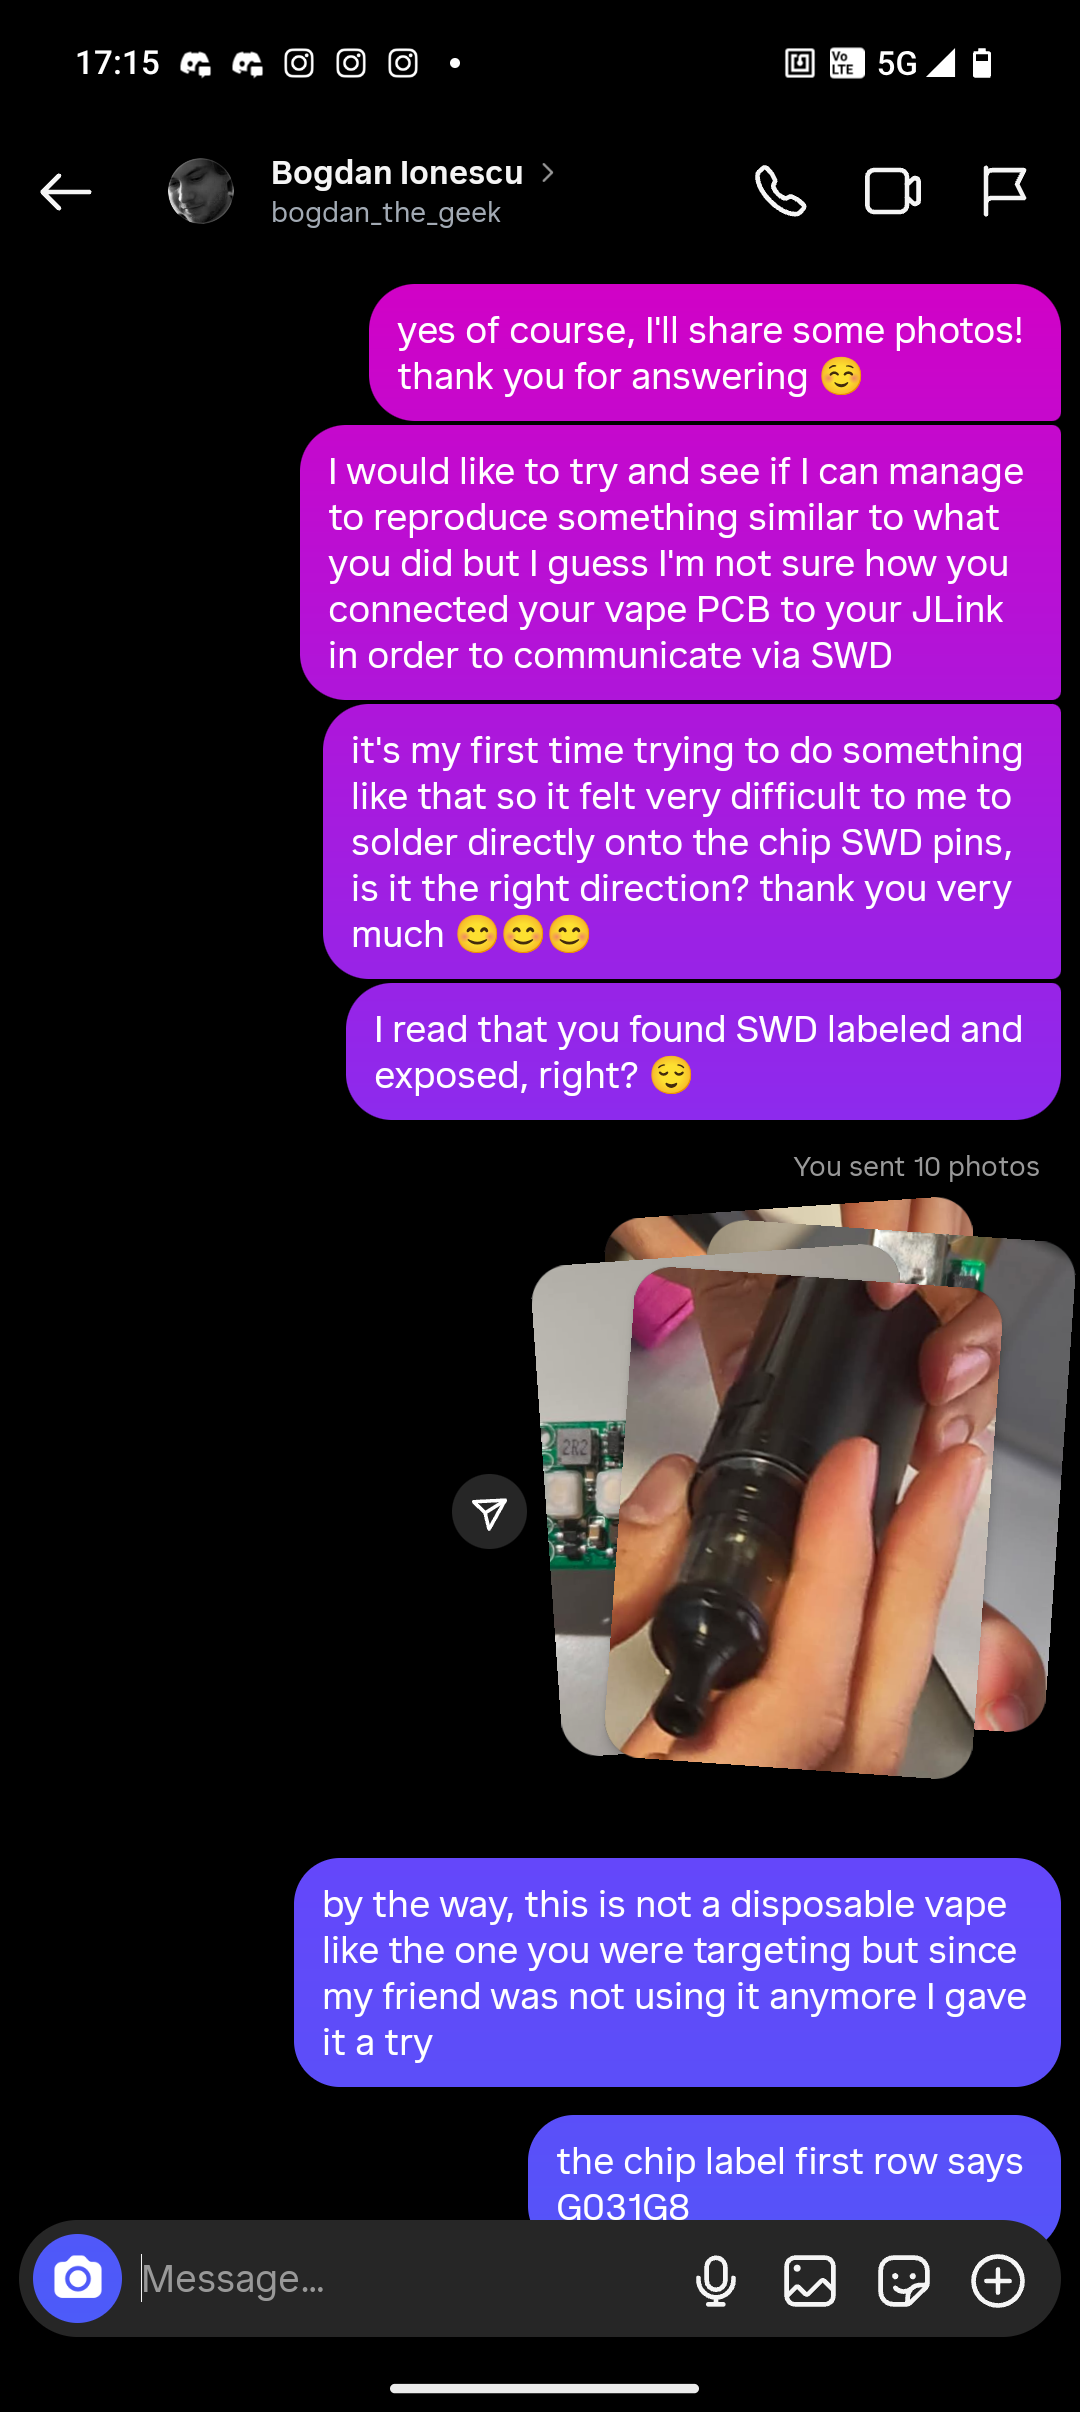
\includegraphics[width=0.3\linewidth]{assets/bogdan_2}}\hfill
  				\subfloat{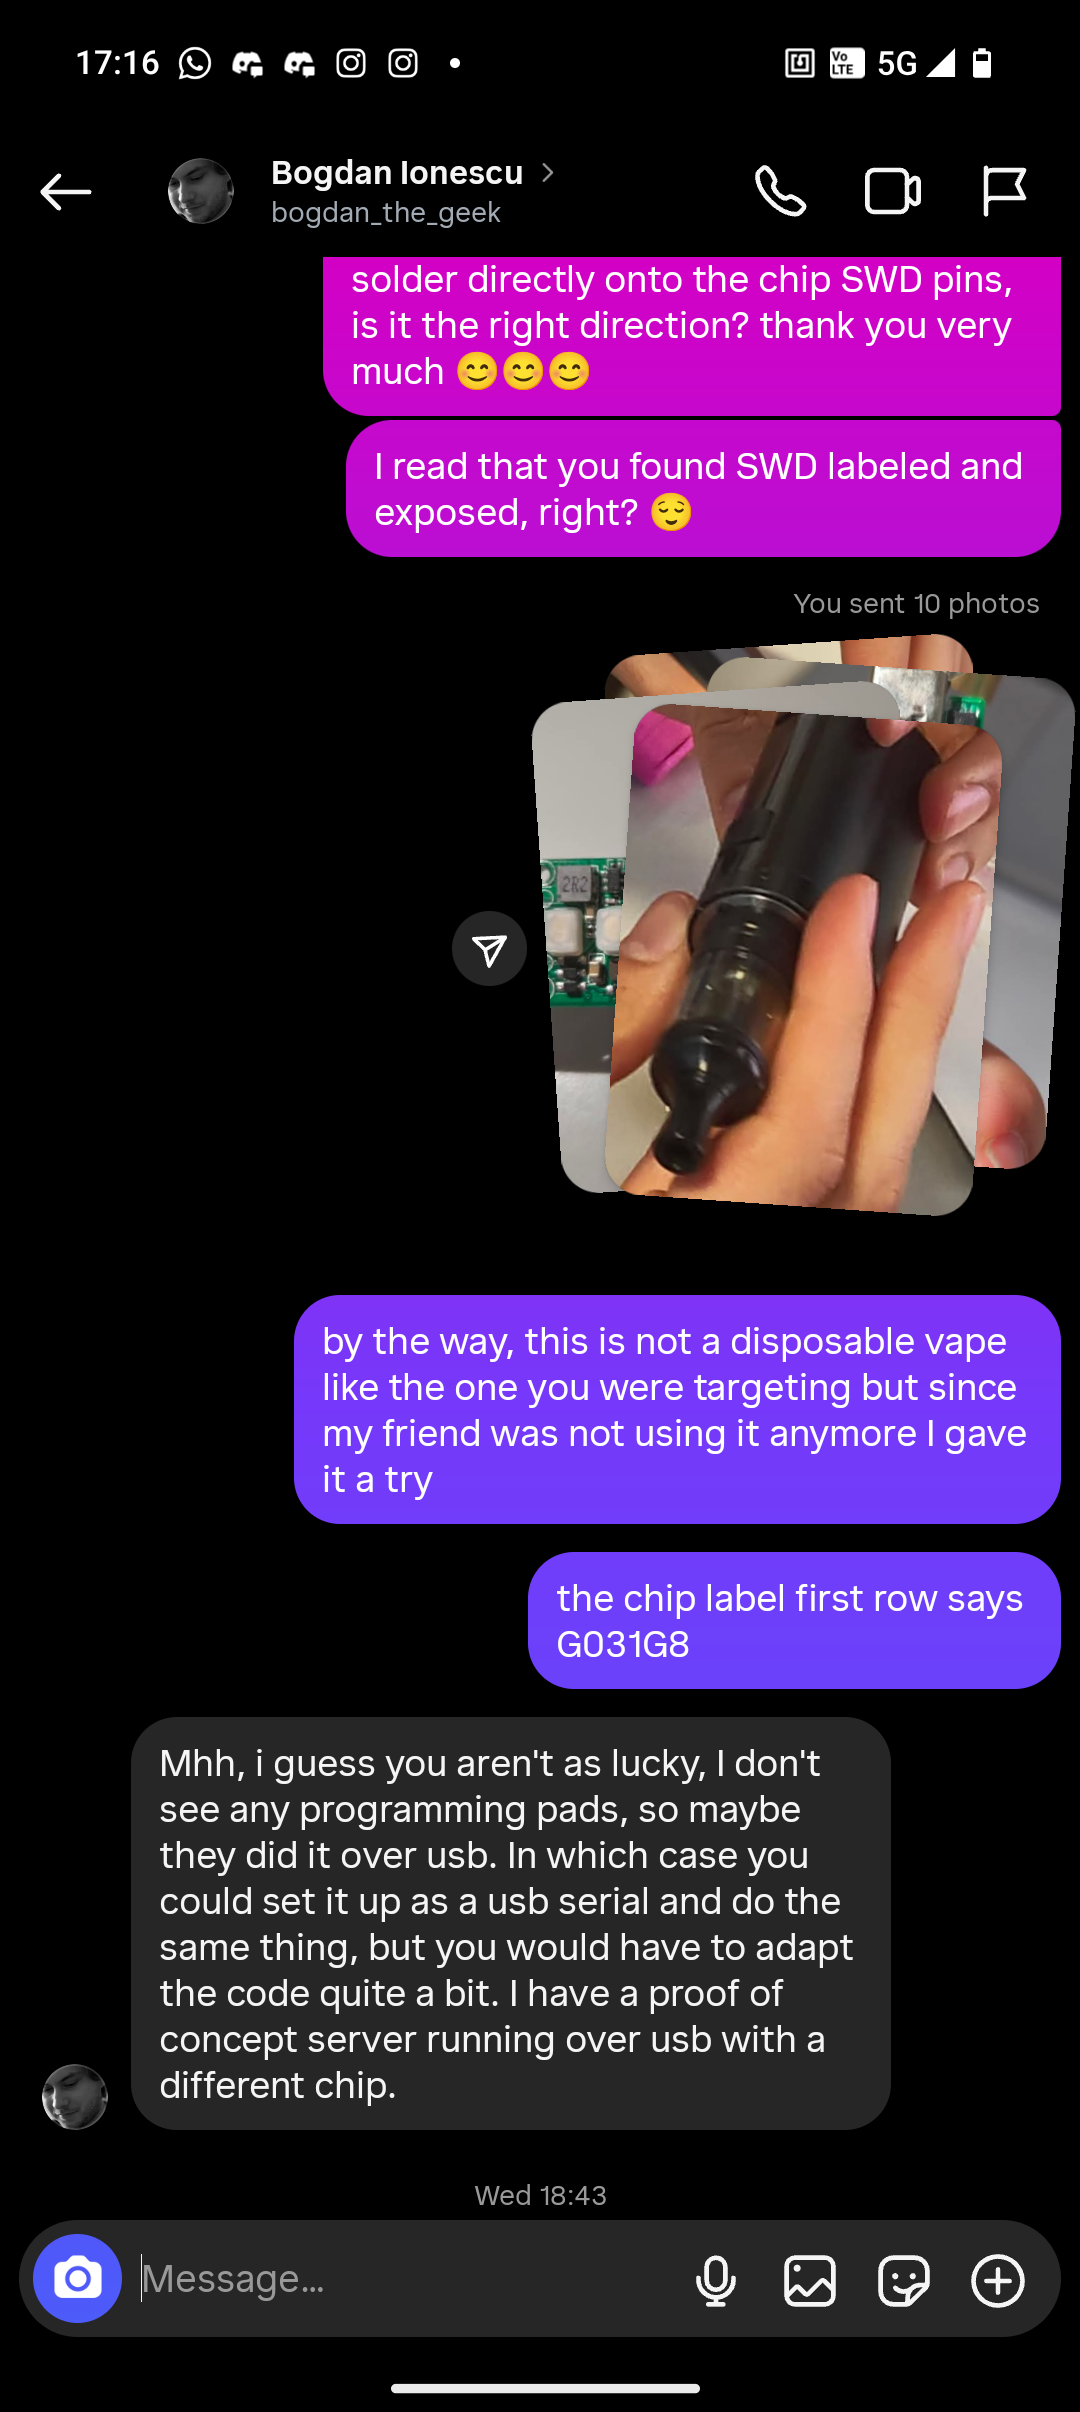
\includegraphics[width=0.3\linewidth]{assets/bogdan_3}}\hfill%
			\end{figure}
		\end{frame}
	\end{NoHyper}

	\begin{NoHyper}
        \begin{frame}{Problem 3 - Solution}
					Let's book a trip to Sicily to clarify our minds (jokes aside, we had a ""work conference"")
					\begin{figure}
						\centering
						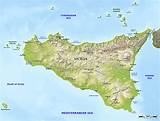
\includegraphics[width=.6\textwidth]{assets/sicily.jpg}
					\end{figure}
		\end{frame}
	\end{NoHyper}

   \begin{NoHyper}
			\section{Atto I}
			\frame{\sectionpage}
	\end{NoHyper}

   \begin{NoHyper}
        \begin{frame}{The target}
			Our target was the Geekbar pulse eVape
			\begin{figure}
				\centering
				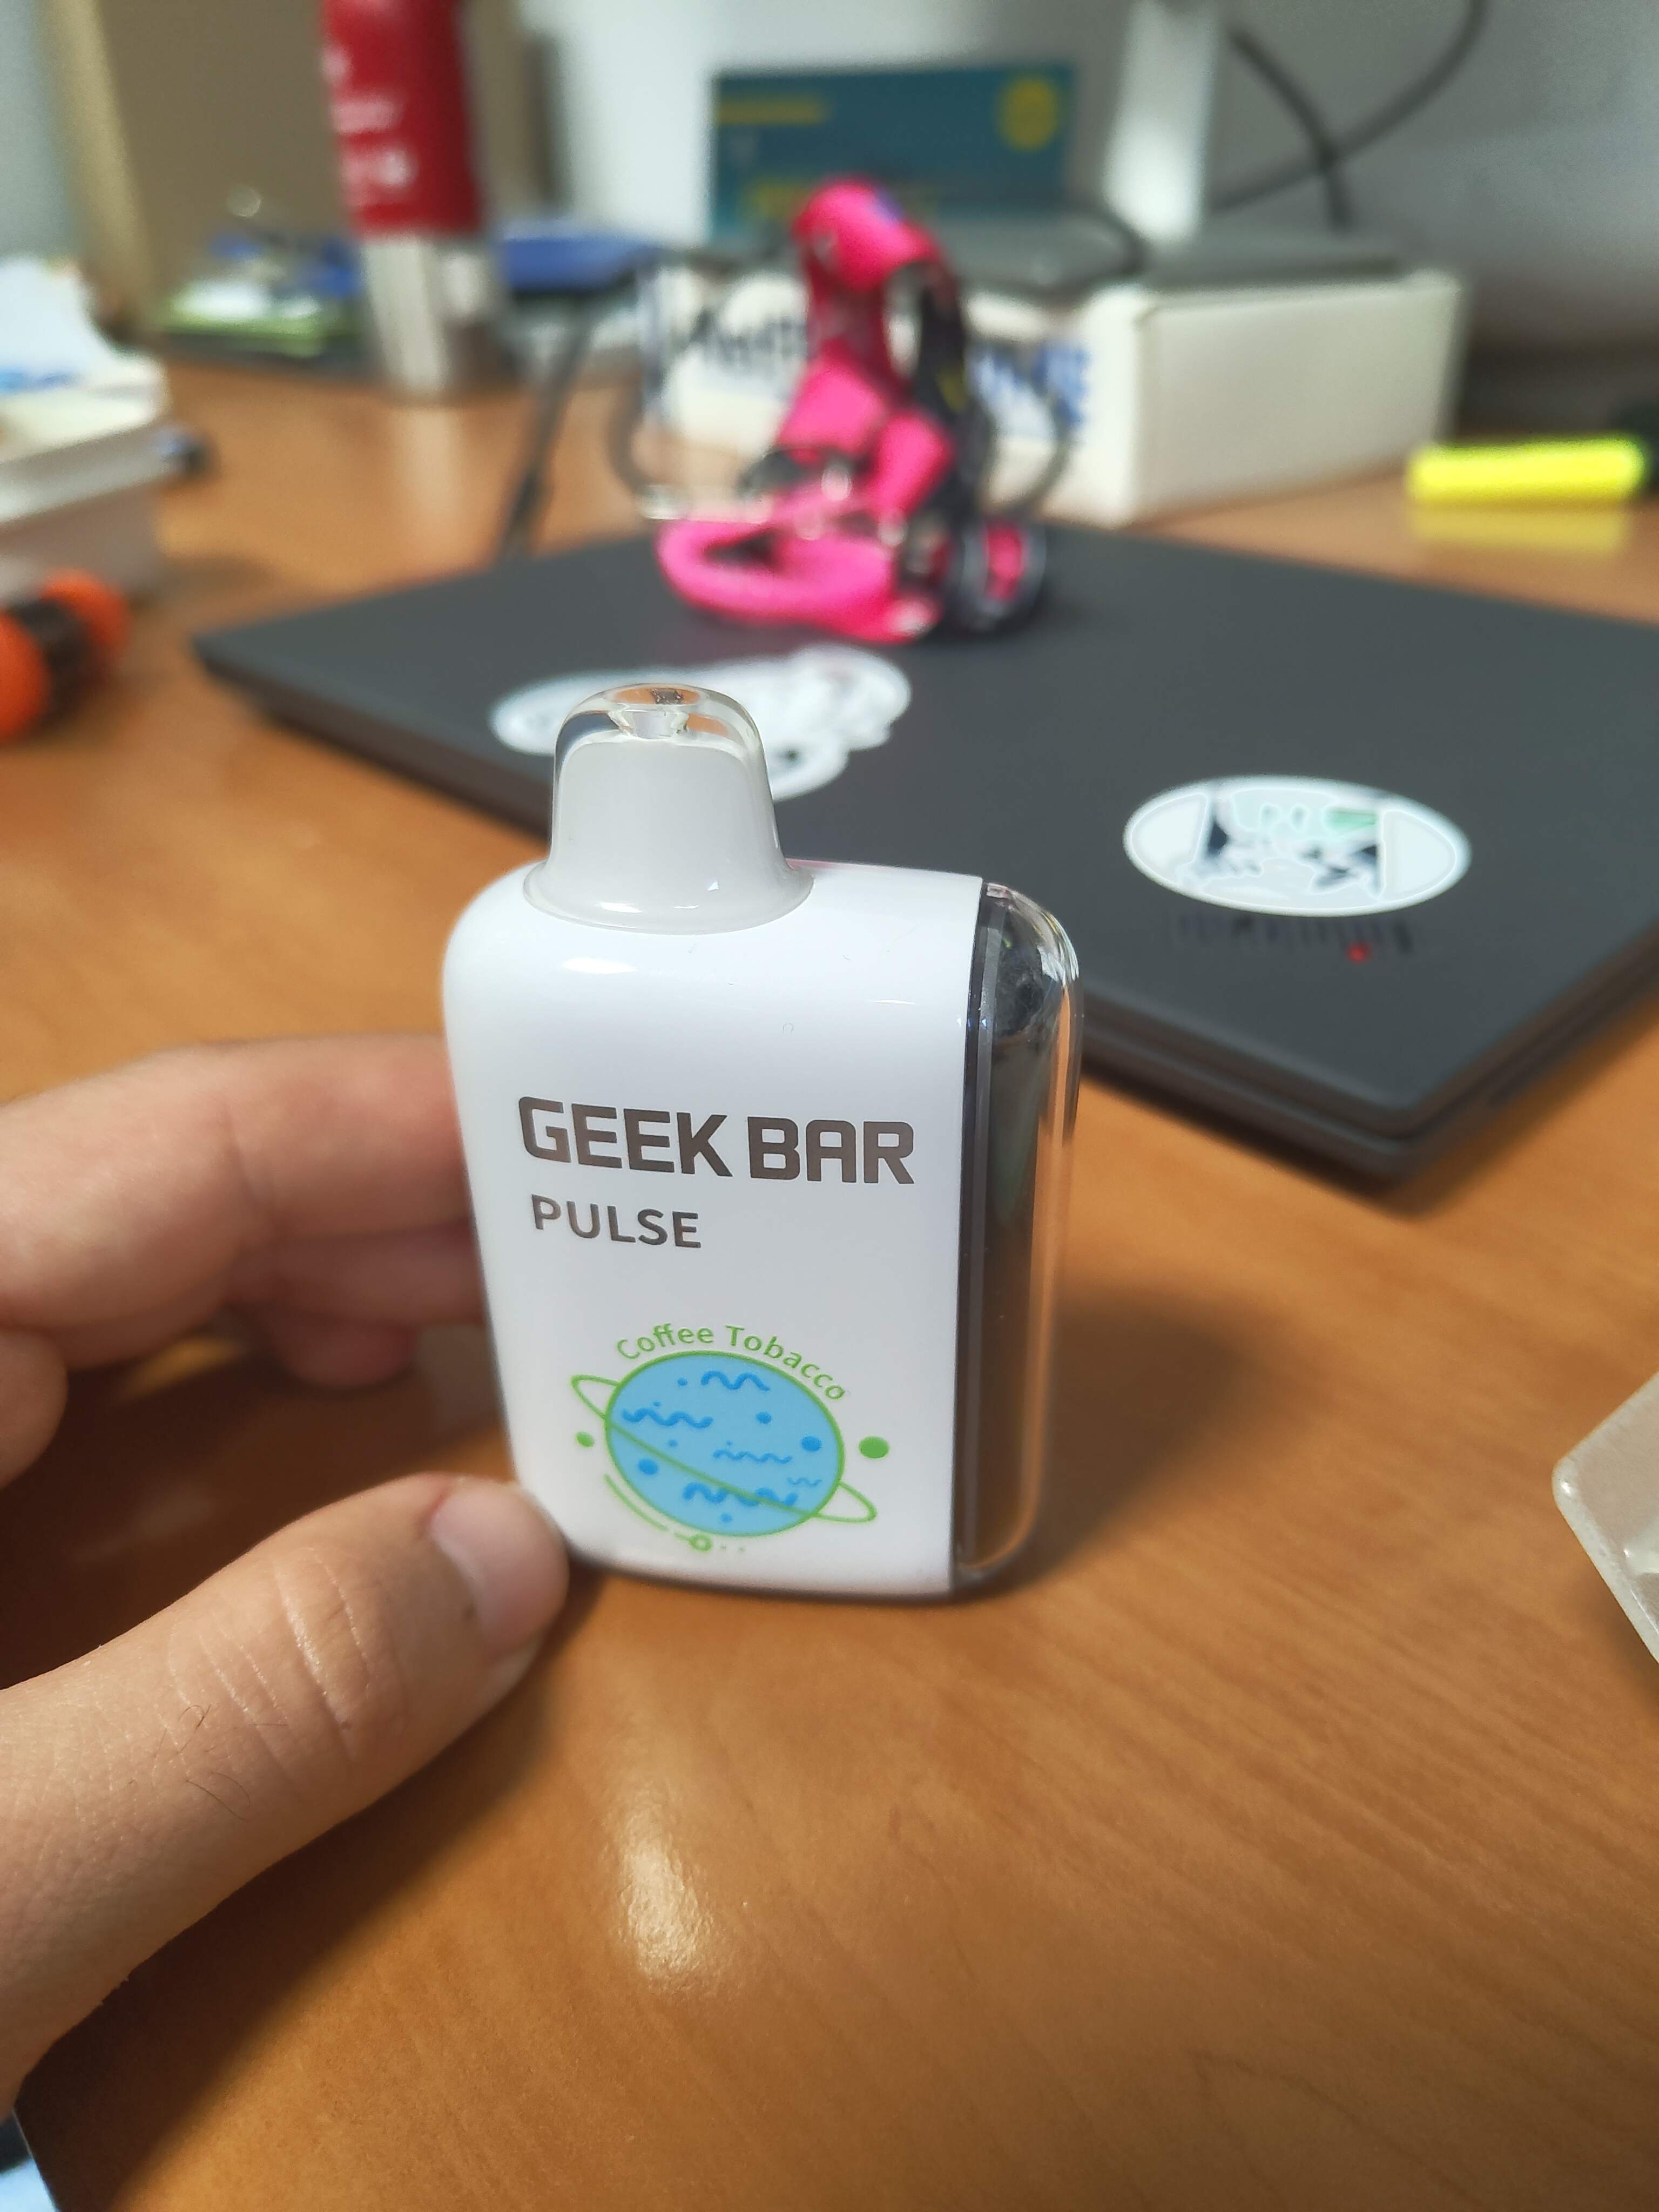
\includegraphics[width=.45\textwidth]{assets/target_1.jpg}
			\end{figure}
		\end{frame}
	\end{NoHyper}

   \begin{NoHyper}
        \begin{frame}{eVape disassembly}
			\begin{figure}[t!]
				\subfloat{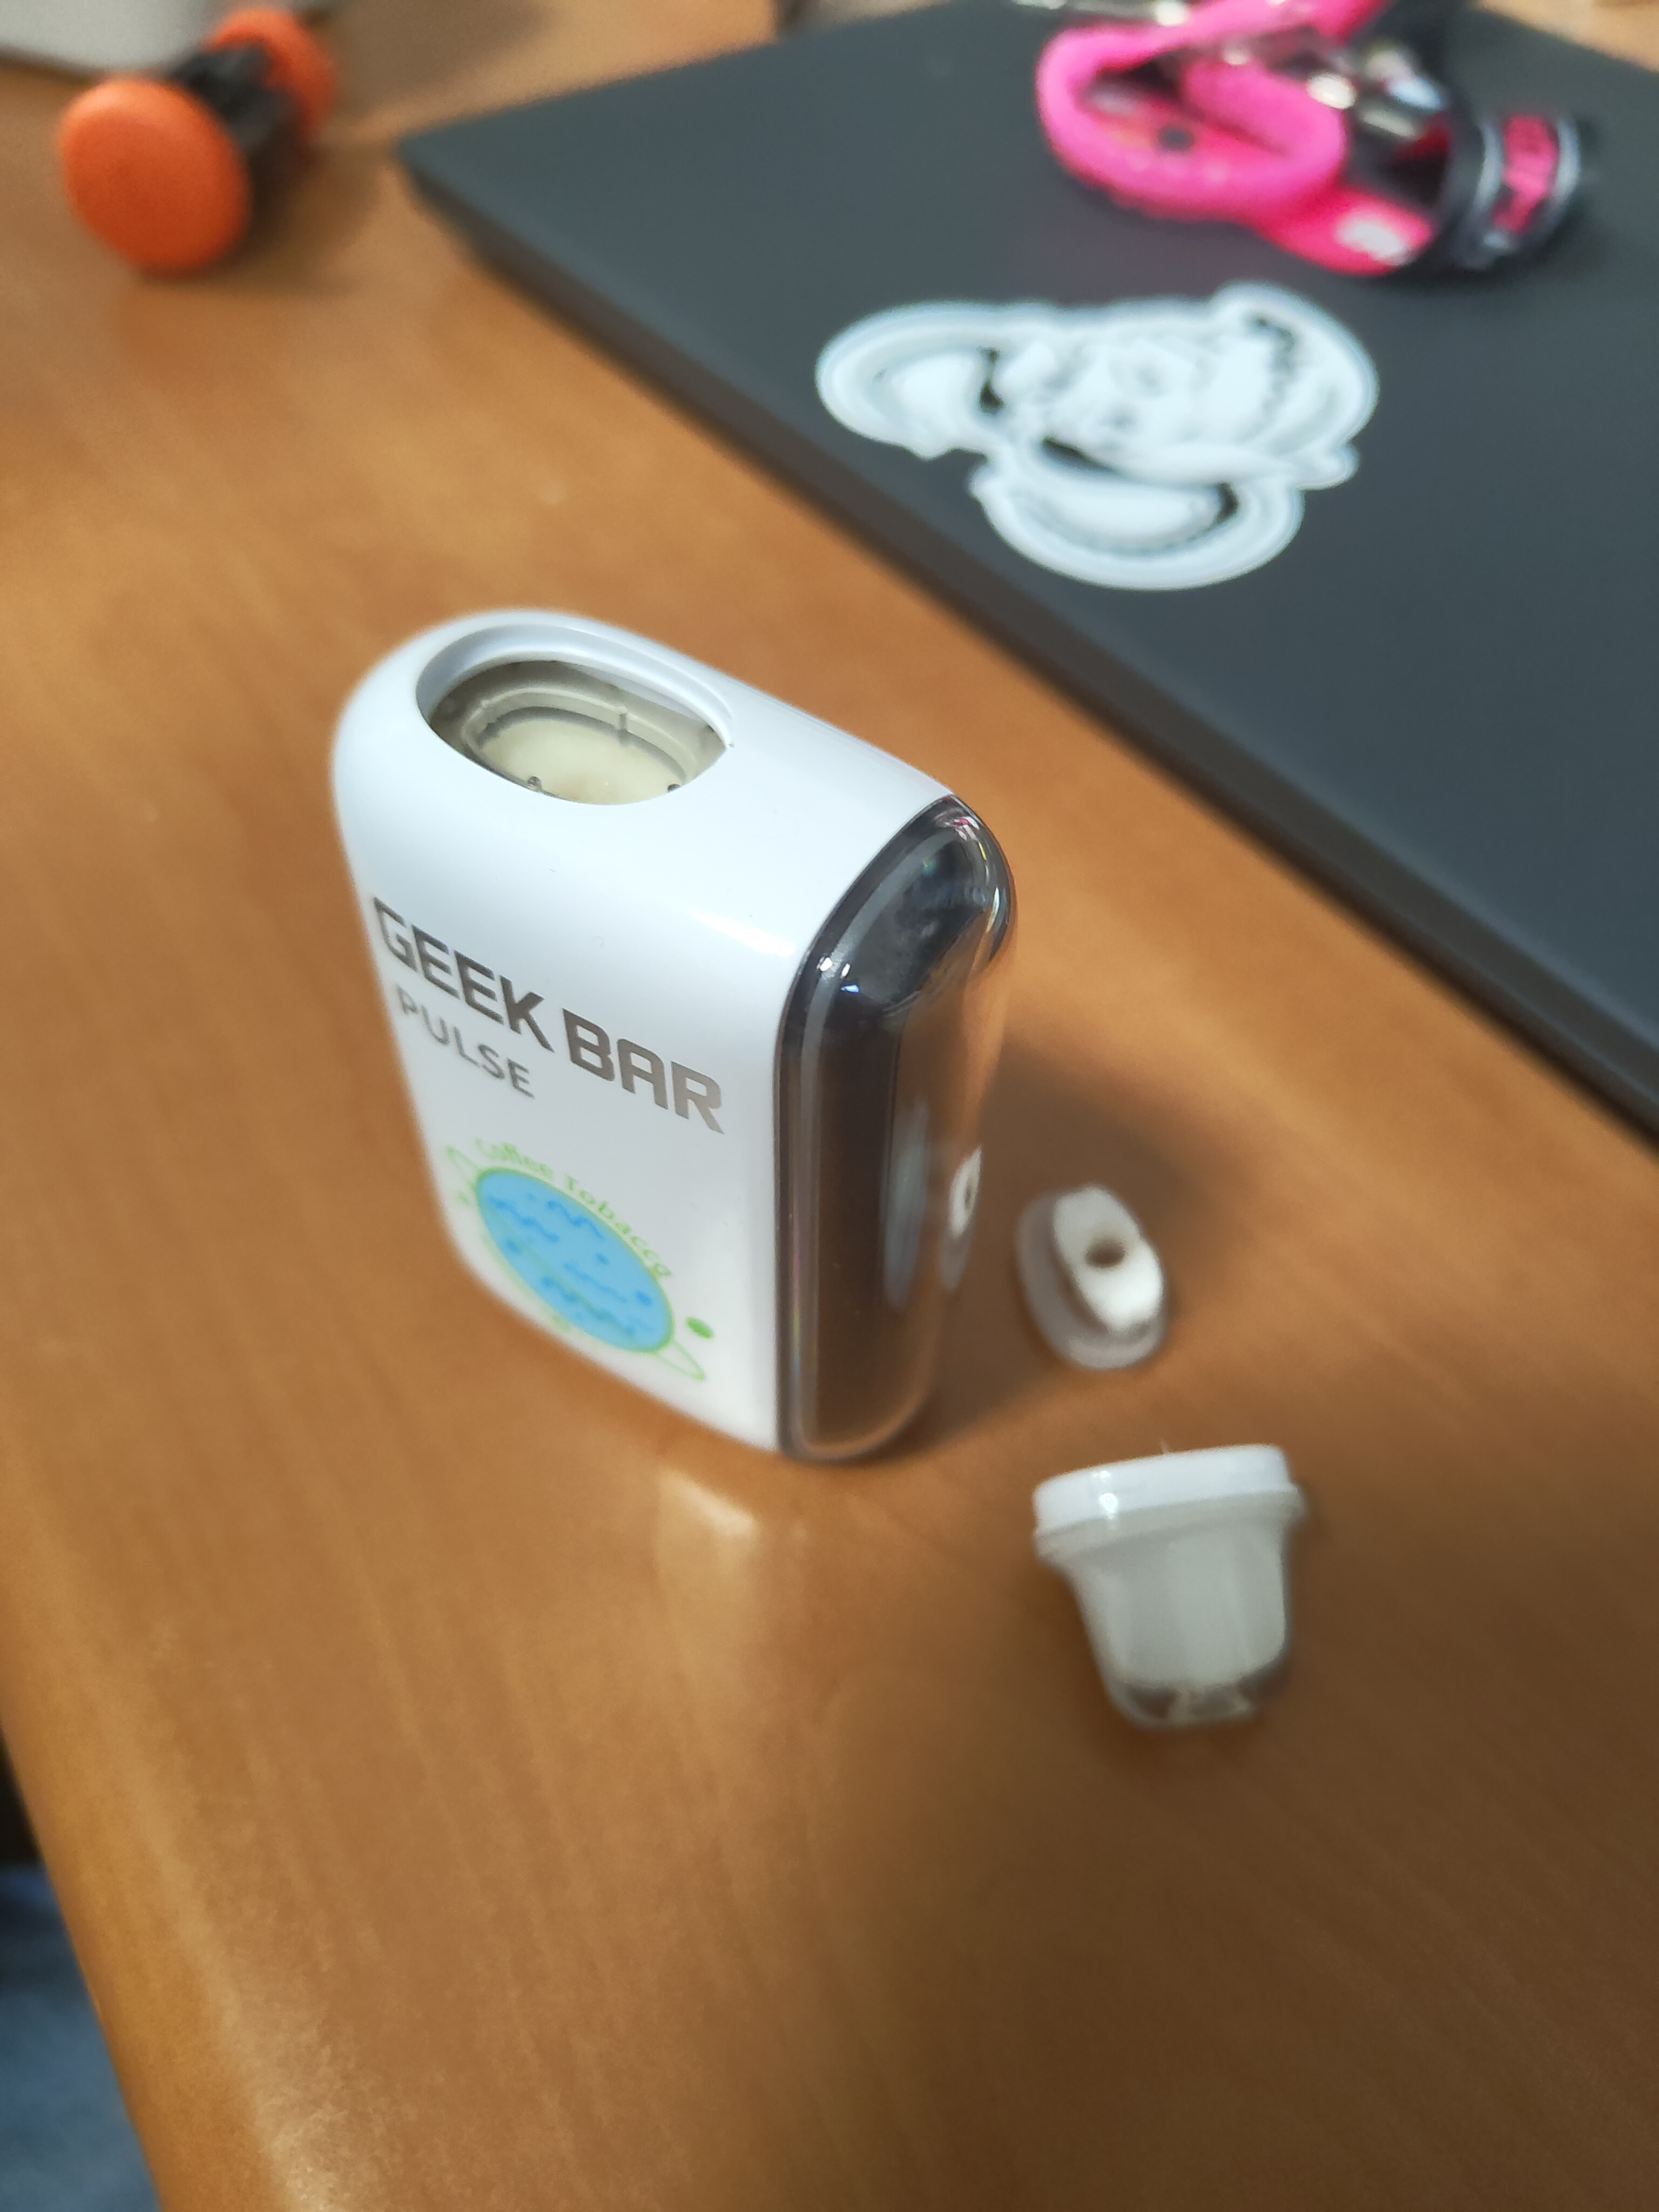
\includegraphics[width=0.3\linewidth]{assets/vape_3.jpg}}\hfill
  				\subfloat{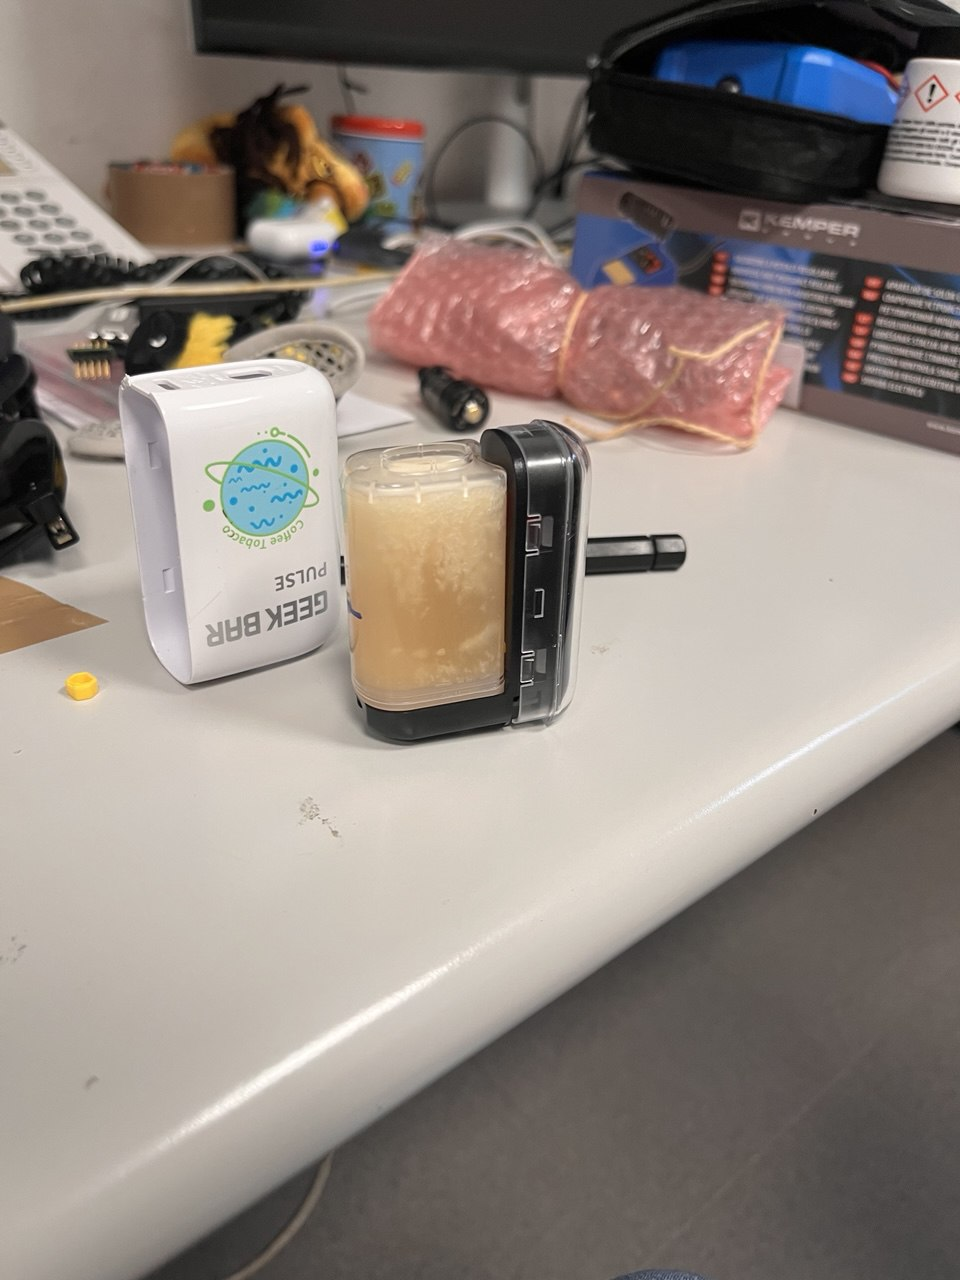
\includegraphics[width=0.3\linewidth]{assets/vape_1.jpg}}\hfill
  				\subfloat{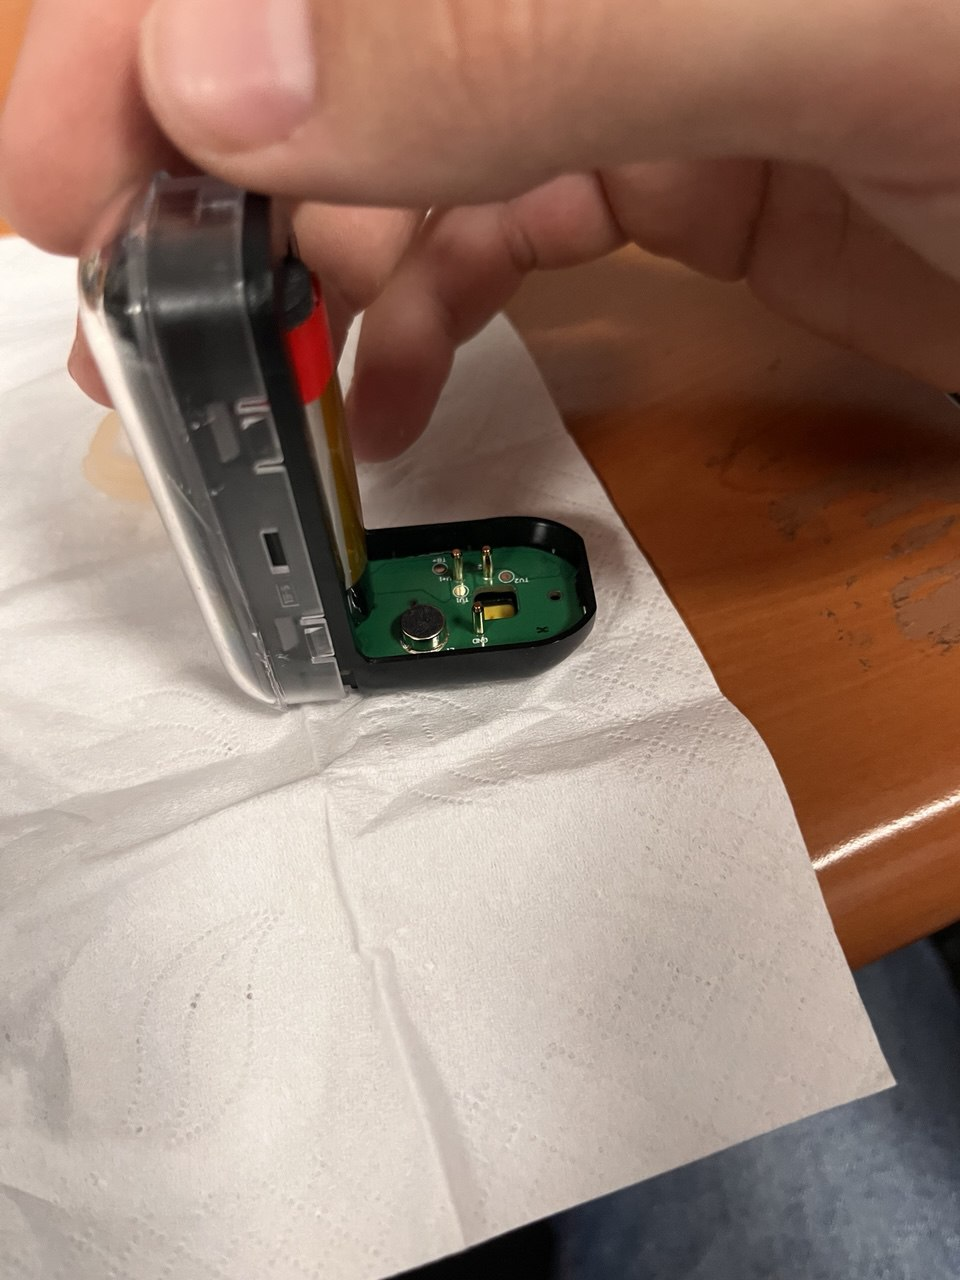
\includegraphics[width=0.3\linewidth]{assets/vape_2.jpg}}\hfill%
			\end{figure}
		\end{frame}
	\end{NoHyper}

   \begin{NoHyper}
        \begin{frame}{eVape disassembly}
			We actually were lucky this time! The SoC was a Puya model, exactly what we were looking for
			\begin{figure}[t!]
				\subfloat{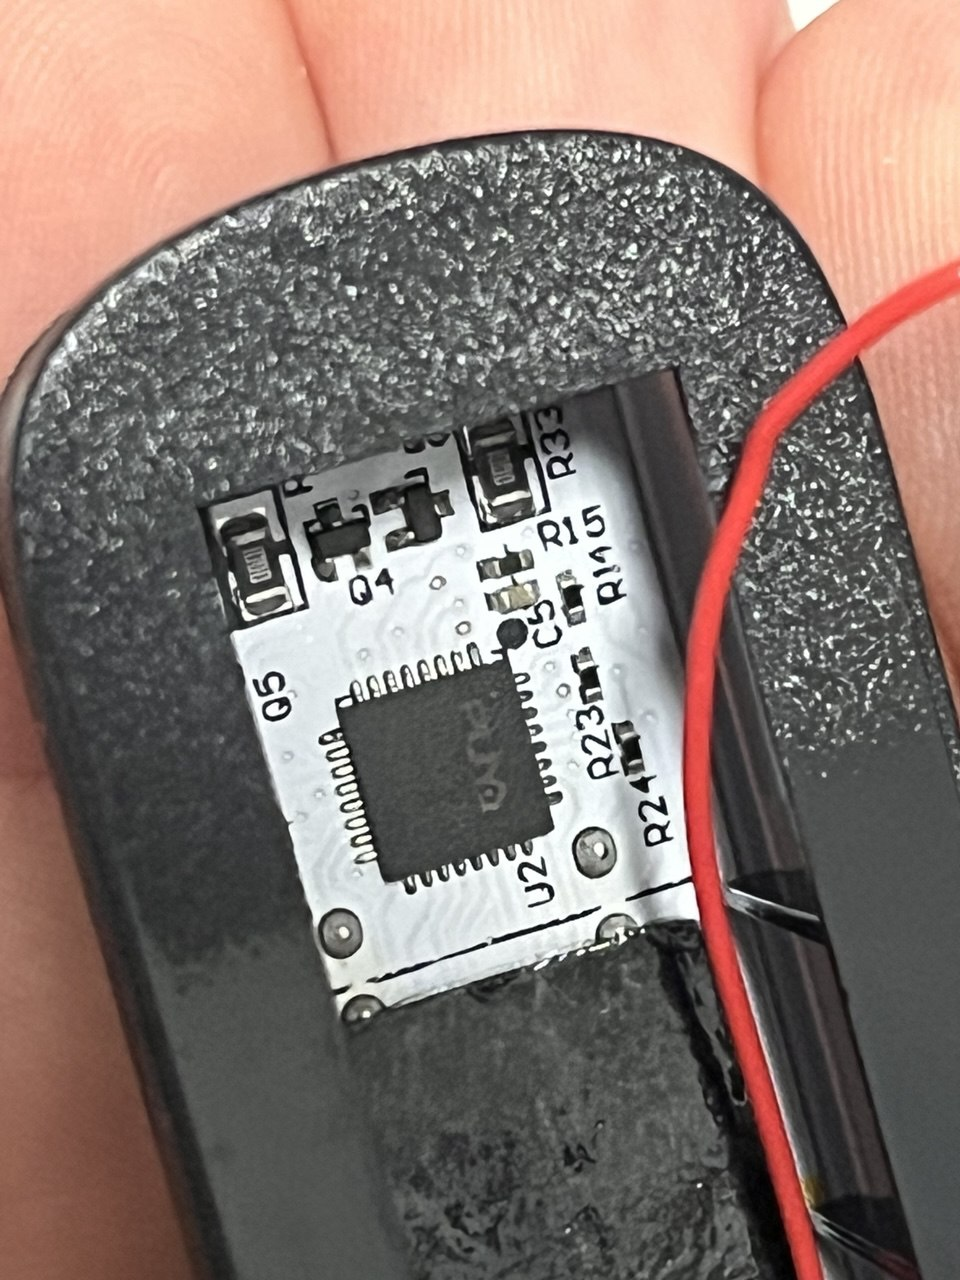
\includegraphics[width=0.3\linewidth]{assets/puya_1.jpg}}\hfill
  				\subfloat{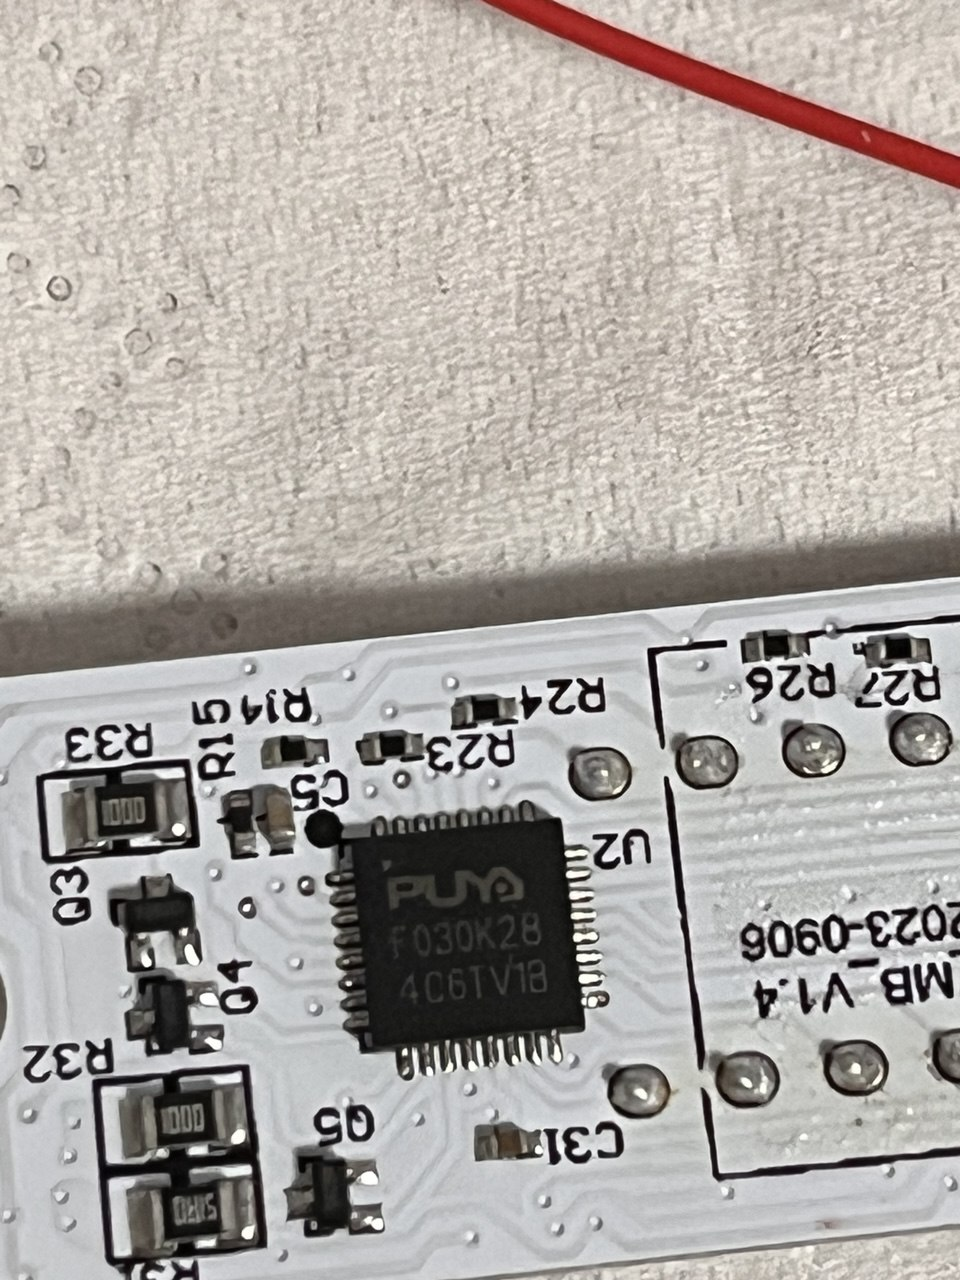
\includegraphics[width=0.3\linewidth]{assets/puya_2.jpg}}\hfill
  				\subfloat{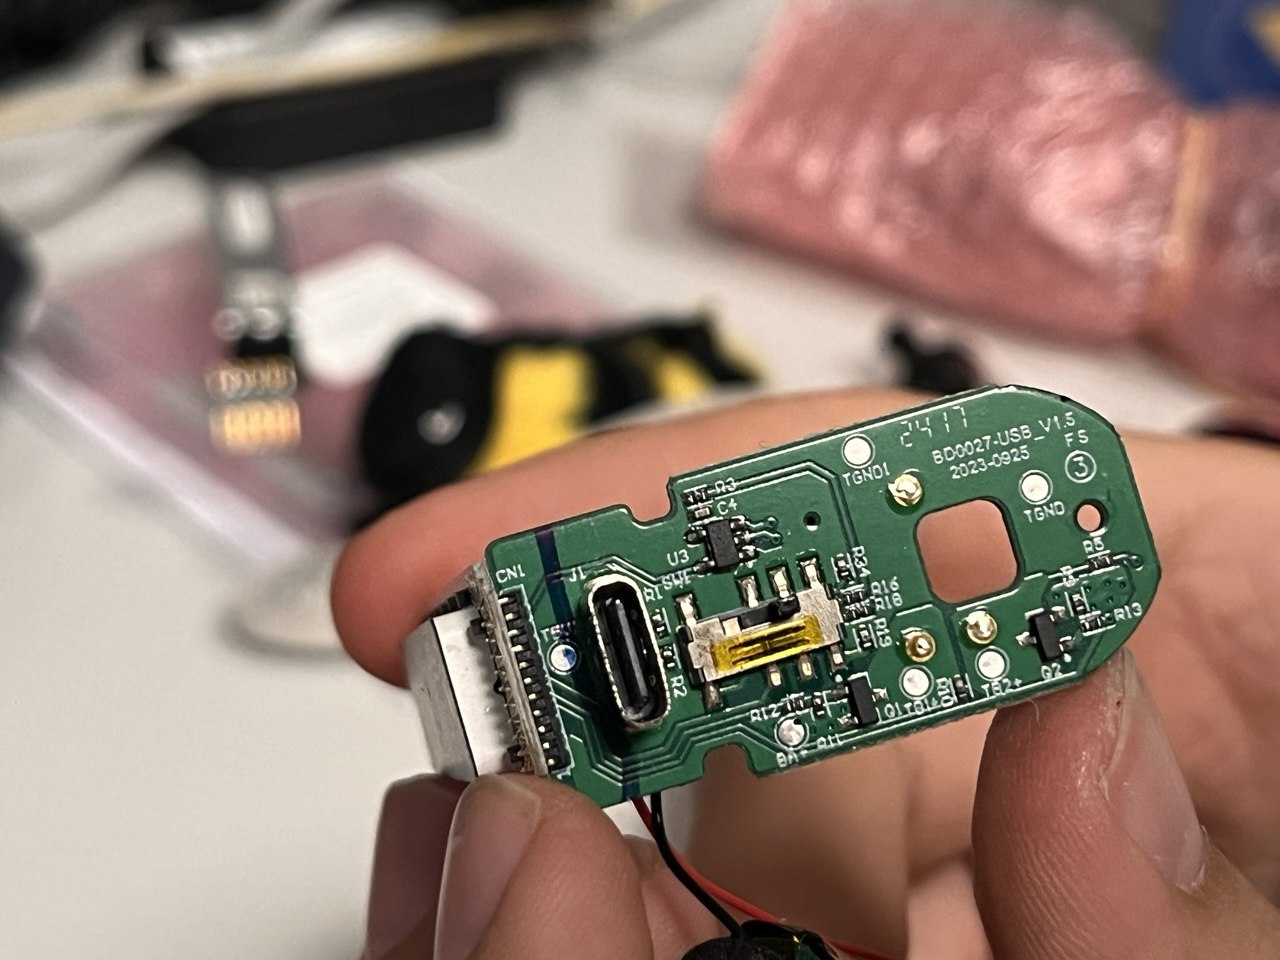
\includegraphics[width=0.3\linewidth]{assets/usbc_pcb.jpg}}\hfill%
			\end{figure}
		\end{frame}
	\end{NoHyper}

   \begin{NoHyper}
        \begin{frame}{Puya model OSINT}
		\begin{minipage}[b]{.5\textwidth}
			\begin{itemize}
				\item By looking around on the internet, we found out that our model was of the \texttt{Puya-F32030xx} family
				\item We tried to lookup for any datasheet around on the internet
			\end{itemize}
		\end{minipage}%
		\begin{minipage}[b]{.5\textwidth}
			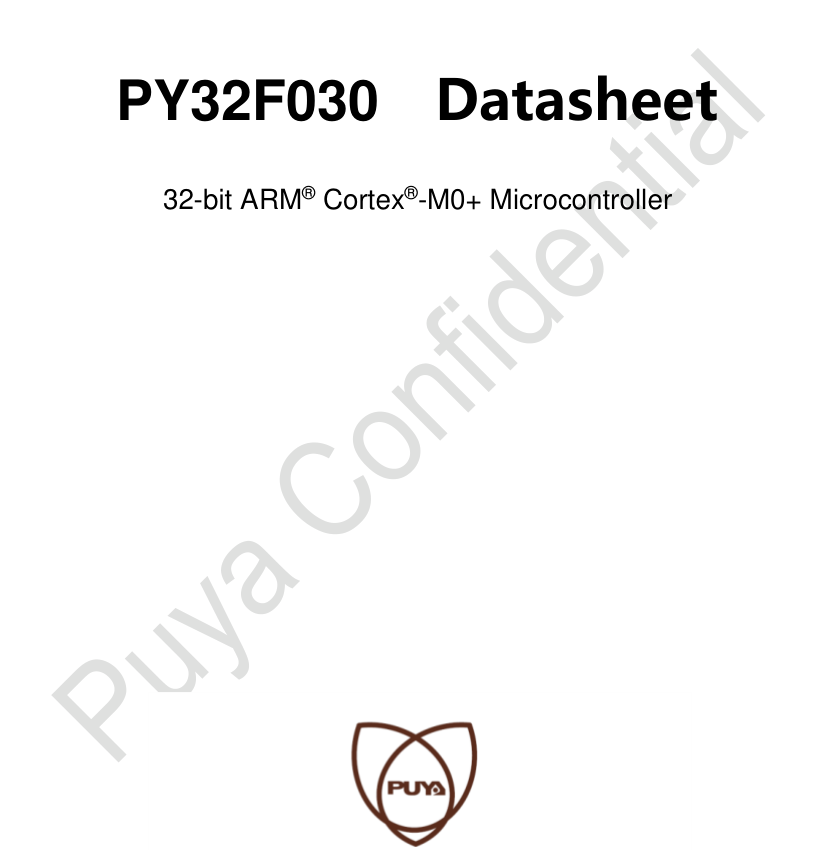
\includegraphics[width=\textwidth]{assets/datasheet_1}
		\end{minipage}%
		\end{frame}
	\end{NoHyper}

   \begin{NoHyper}
        \begin{frame}{Puya model OSINT - pinout}
			The SWD pins we were looking for!
		\begin{minipage}[b]{.5\textwidth}
			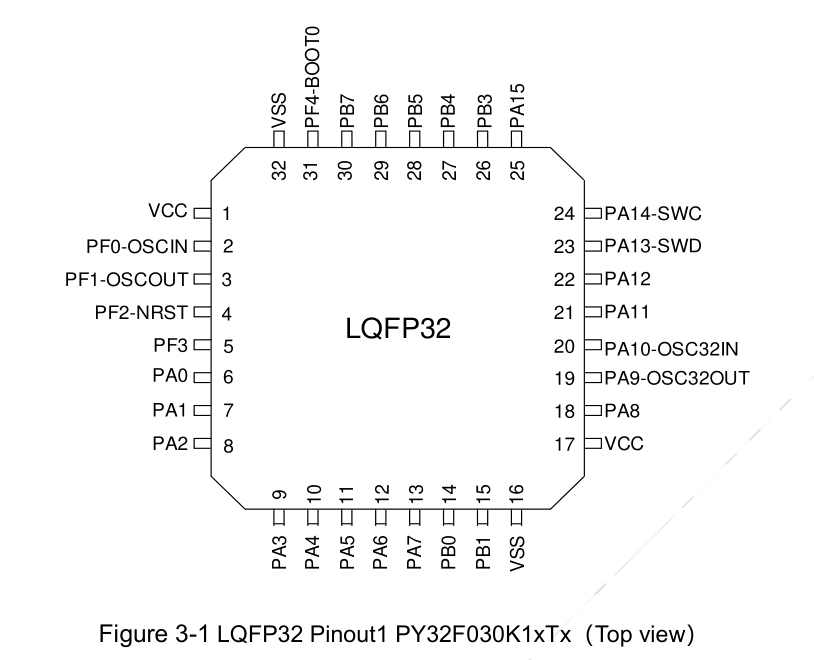
\includegraphics[width=\textwidth]{assets/pinout_1}
		\end{minipage}%
		\begin{minipage}[b]{.5\textwidth}
			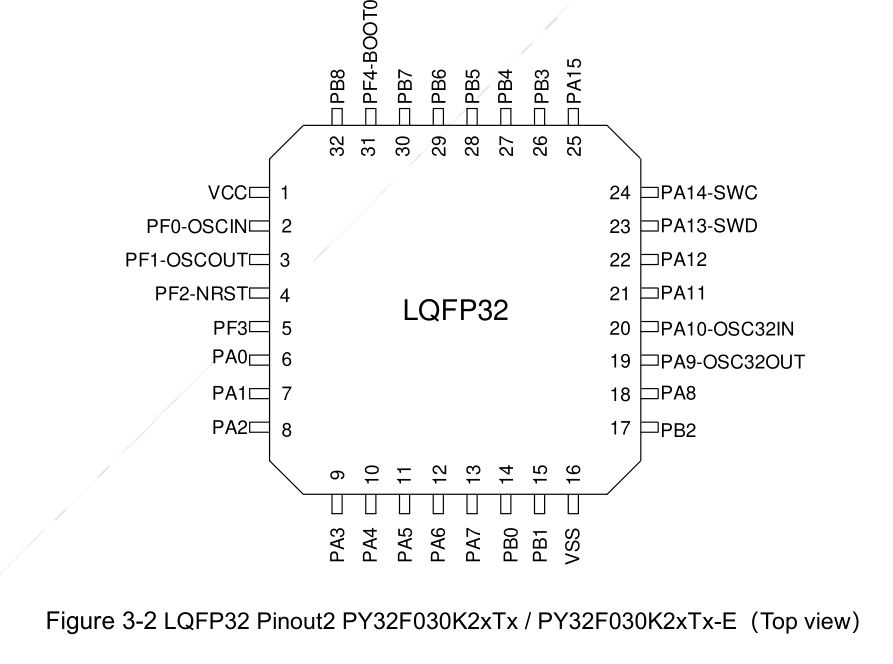
\includegraphics[width=\textwidth]{assets/pinout_2}
		\end{minipage}%
		\end{frame}
	\end{NoHyper}


   \begin{NoHyper}
        \begin{frame}{SWD interaction - first attempt}
			\begin{minipage}[b]{.5\textwidth}
				\vspace{0pt}
				\begin{itemize}
					\item Let's try and use a Raspberry Pi5 first
					\item By leveraging the GPIO pins of the board, we should be capable to attach to the SWD pins
				\end{itemize}
			\end{minipage}%
			\begin{minipage}[b]{.5\textwidth}
				\vspace{0pt}
				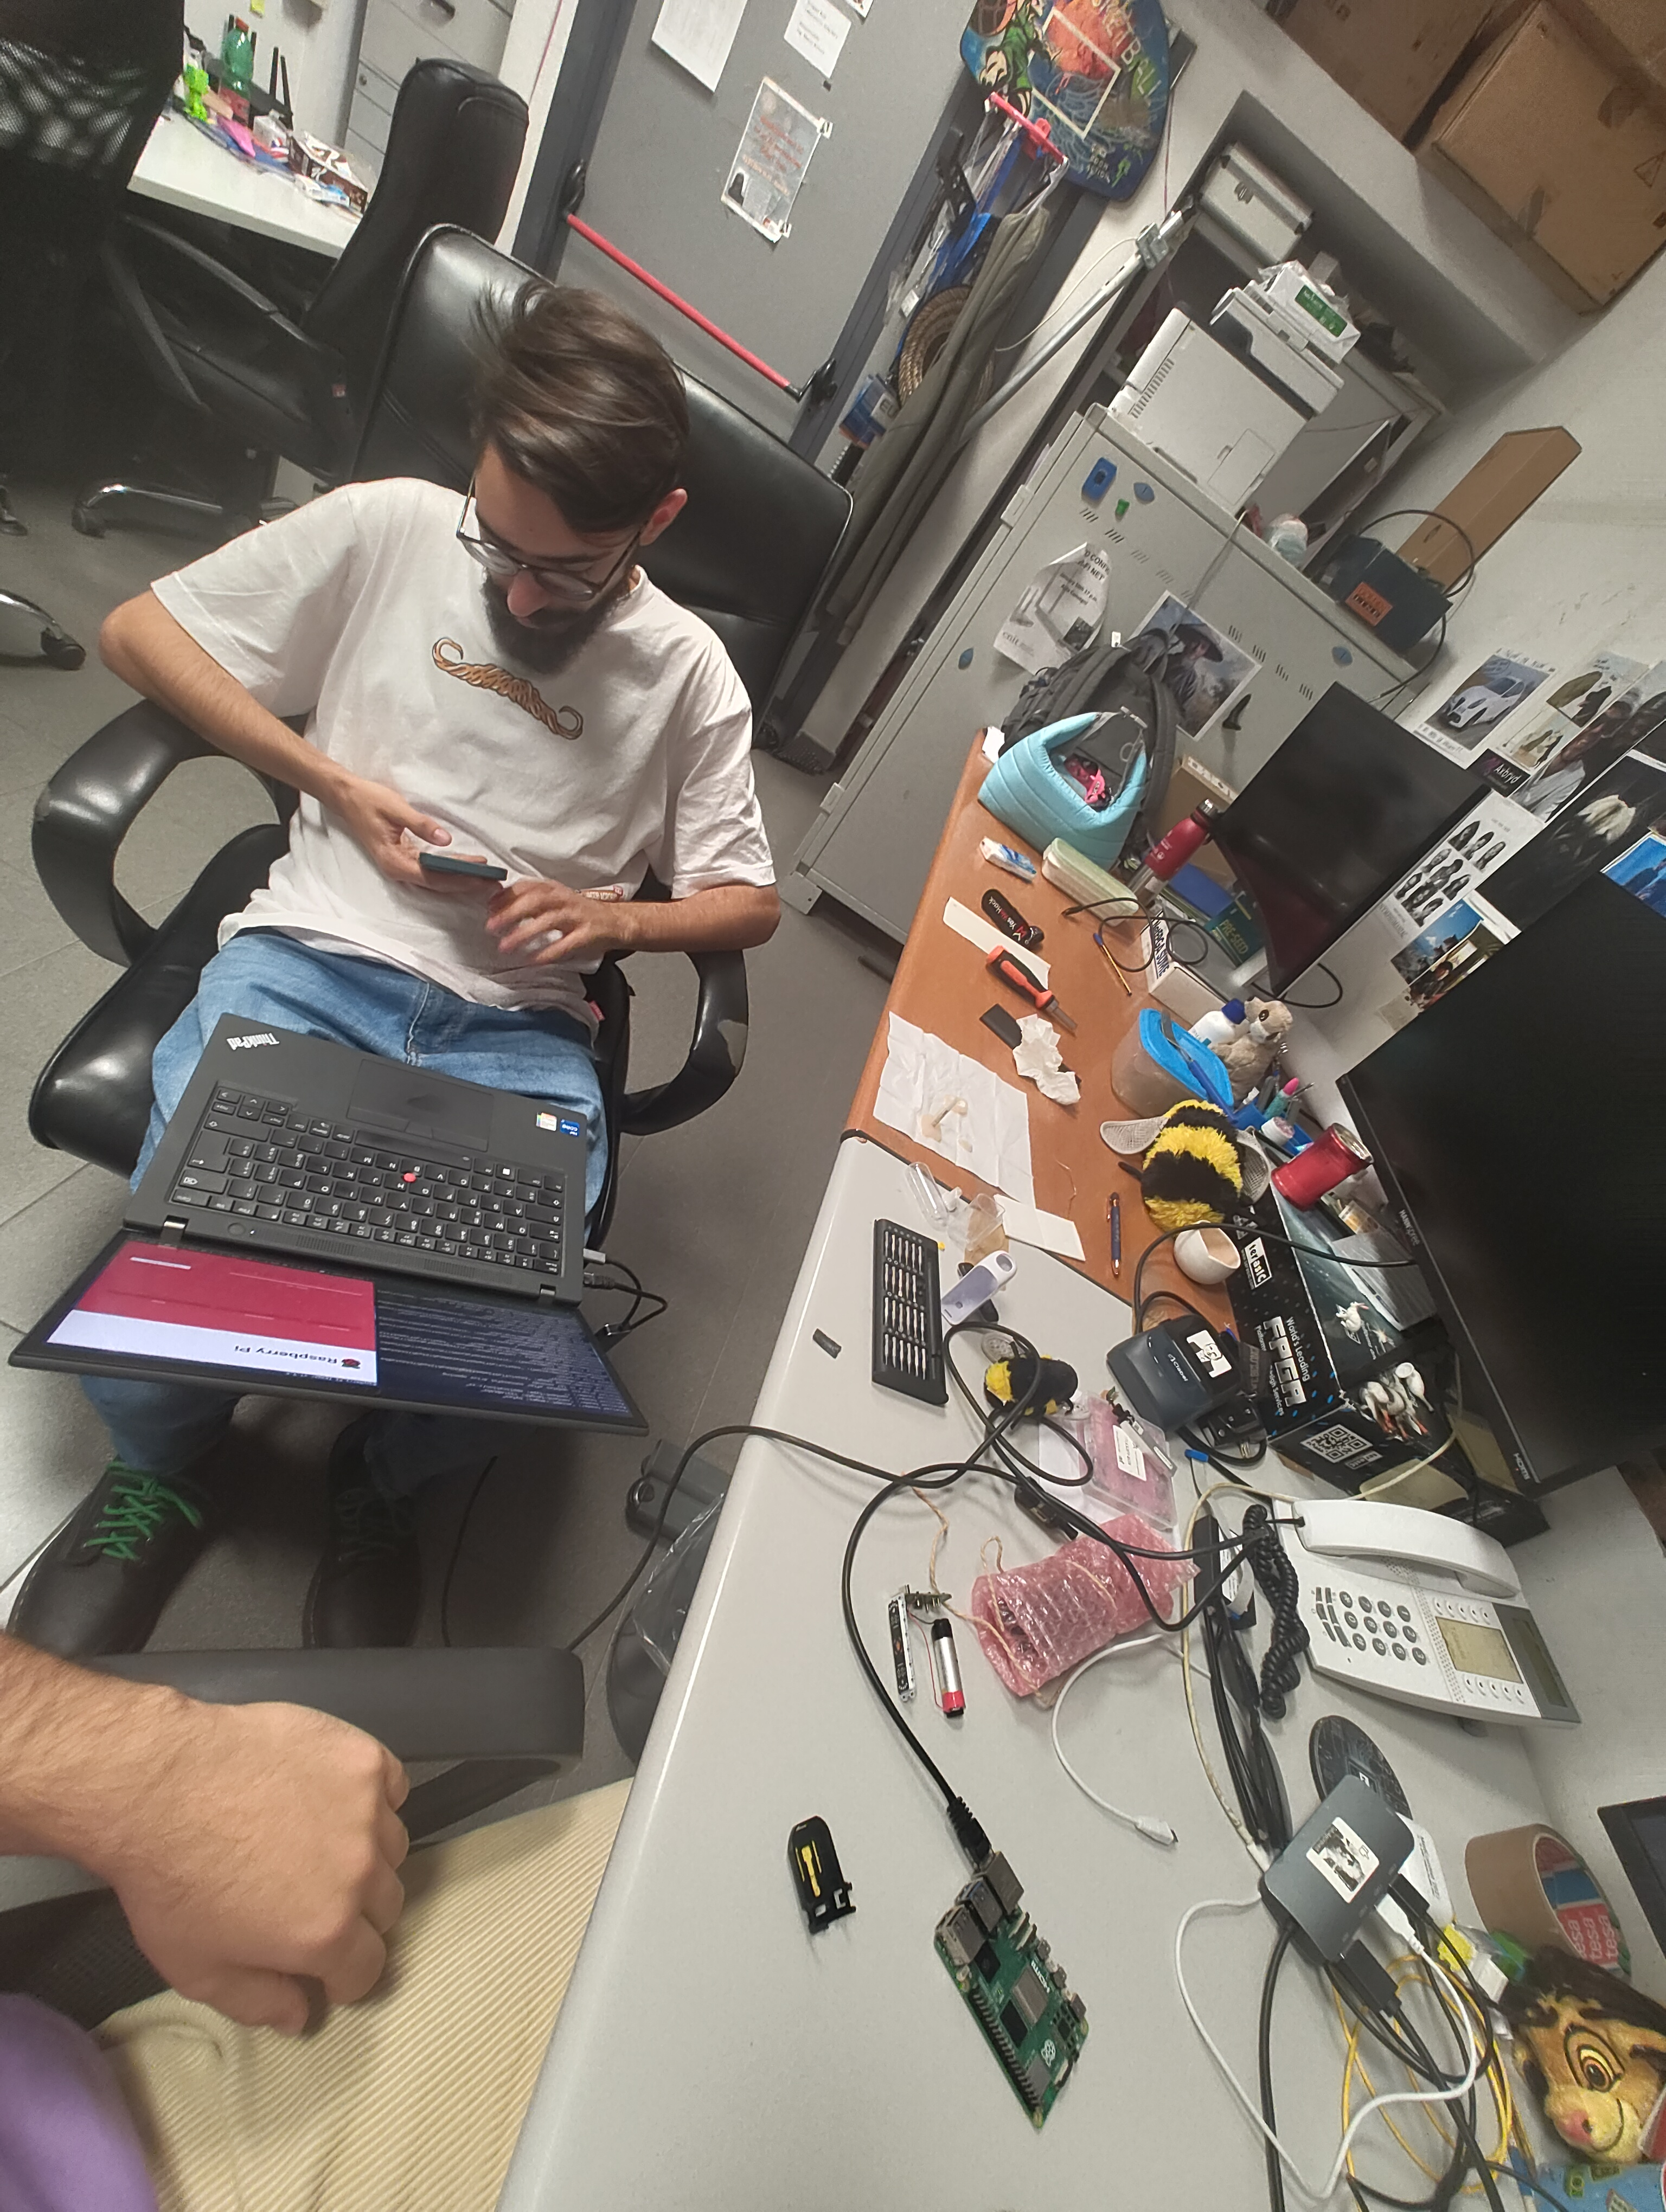
\includegraphics[width=.75\textwidth]{assets/pi5.jpg}
			\end{minipage}
		\end{frame}
	\end{NoHyper}

   \begin{NoHyper}
        \begin{frame}{SWD interaction - first attempt}
			\begin{itemize}
				\item Let's try and use a Raspberry Pi5 first
				\item By leveraging the GPIO pins of the board, we should be capable to attach to the SWD pins
				\item Tools we needed
					\begin{itemize}
						\item Raspberry Pi5 OS
						\item Raspberry PI5 pinout for SWD
						\item openocd
					\end{itemize}
			\end{itemize}
		\end{frame}
	\end{NoHyper}

   \begin{NoHyper}
        \begin{frame}{SWD interaction - first attempt}
			\begin{minipage}[b]{.5\textwidth}
				\begin{itemize}
					\item We managed somehow to understand how to flash a Raspberry Pi5
				\end{itemize}
			\end{minipage}%
			\begin{minipage}[b]{.5\textwidth}
				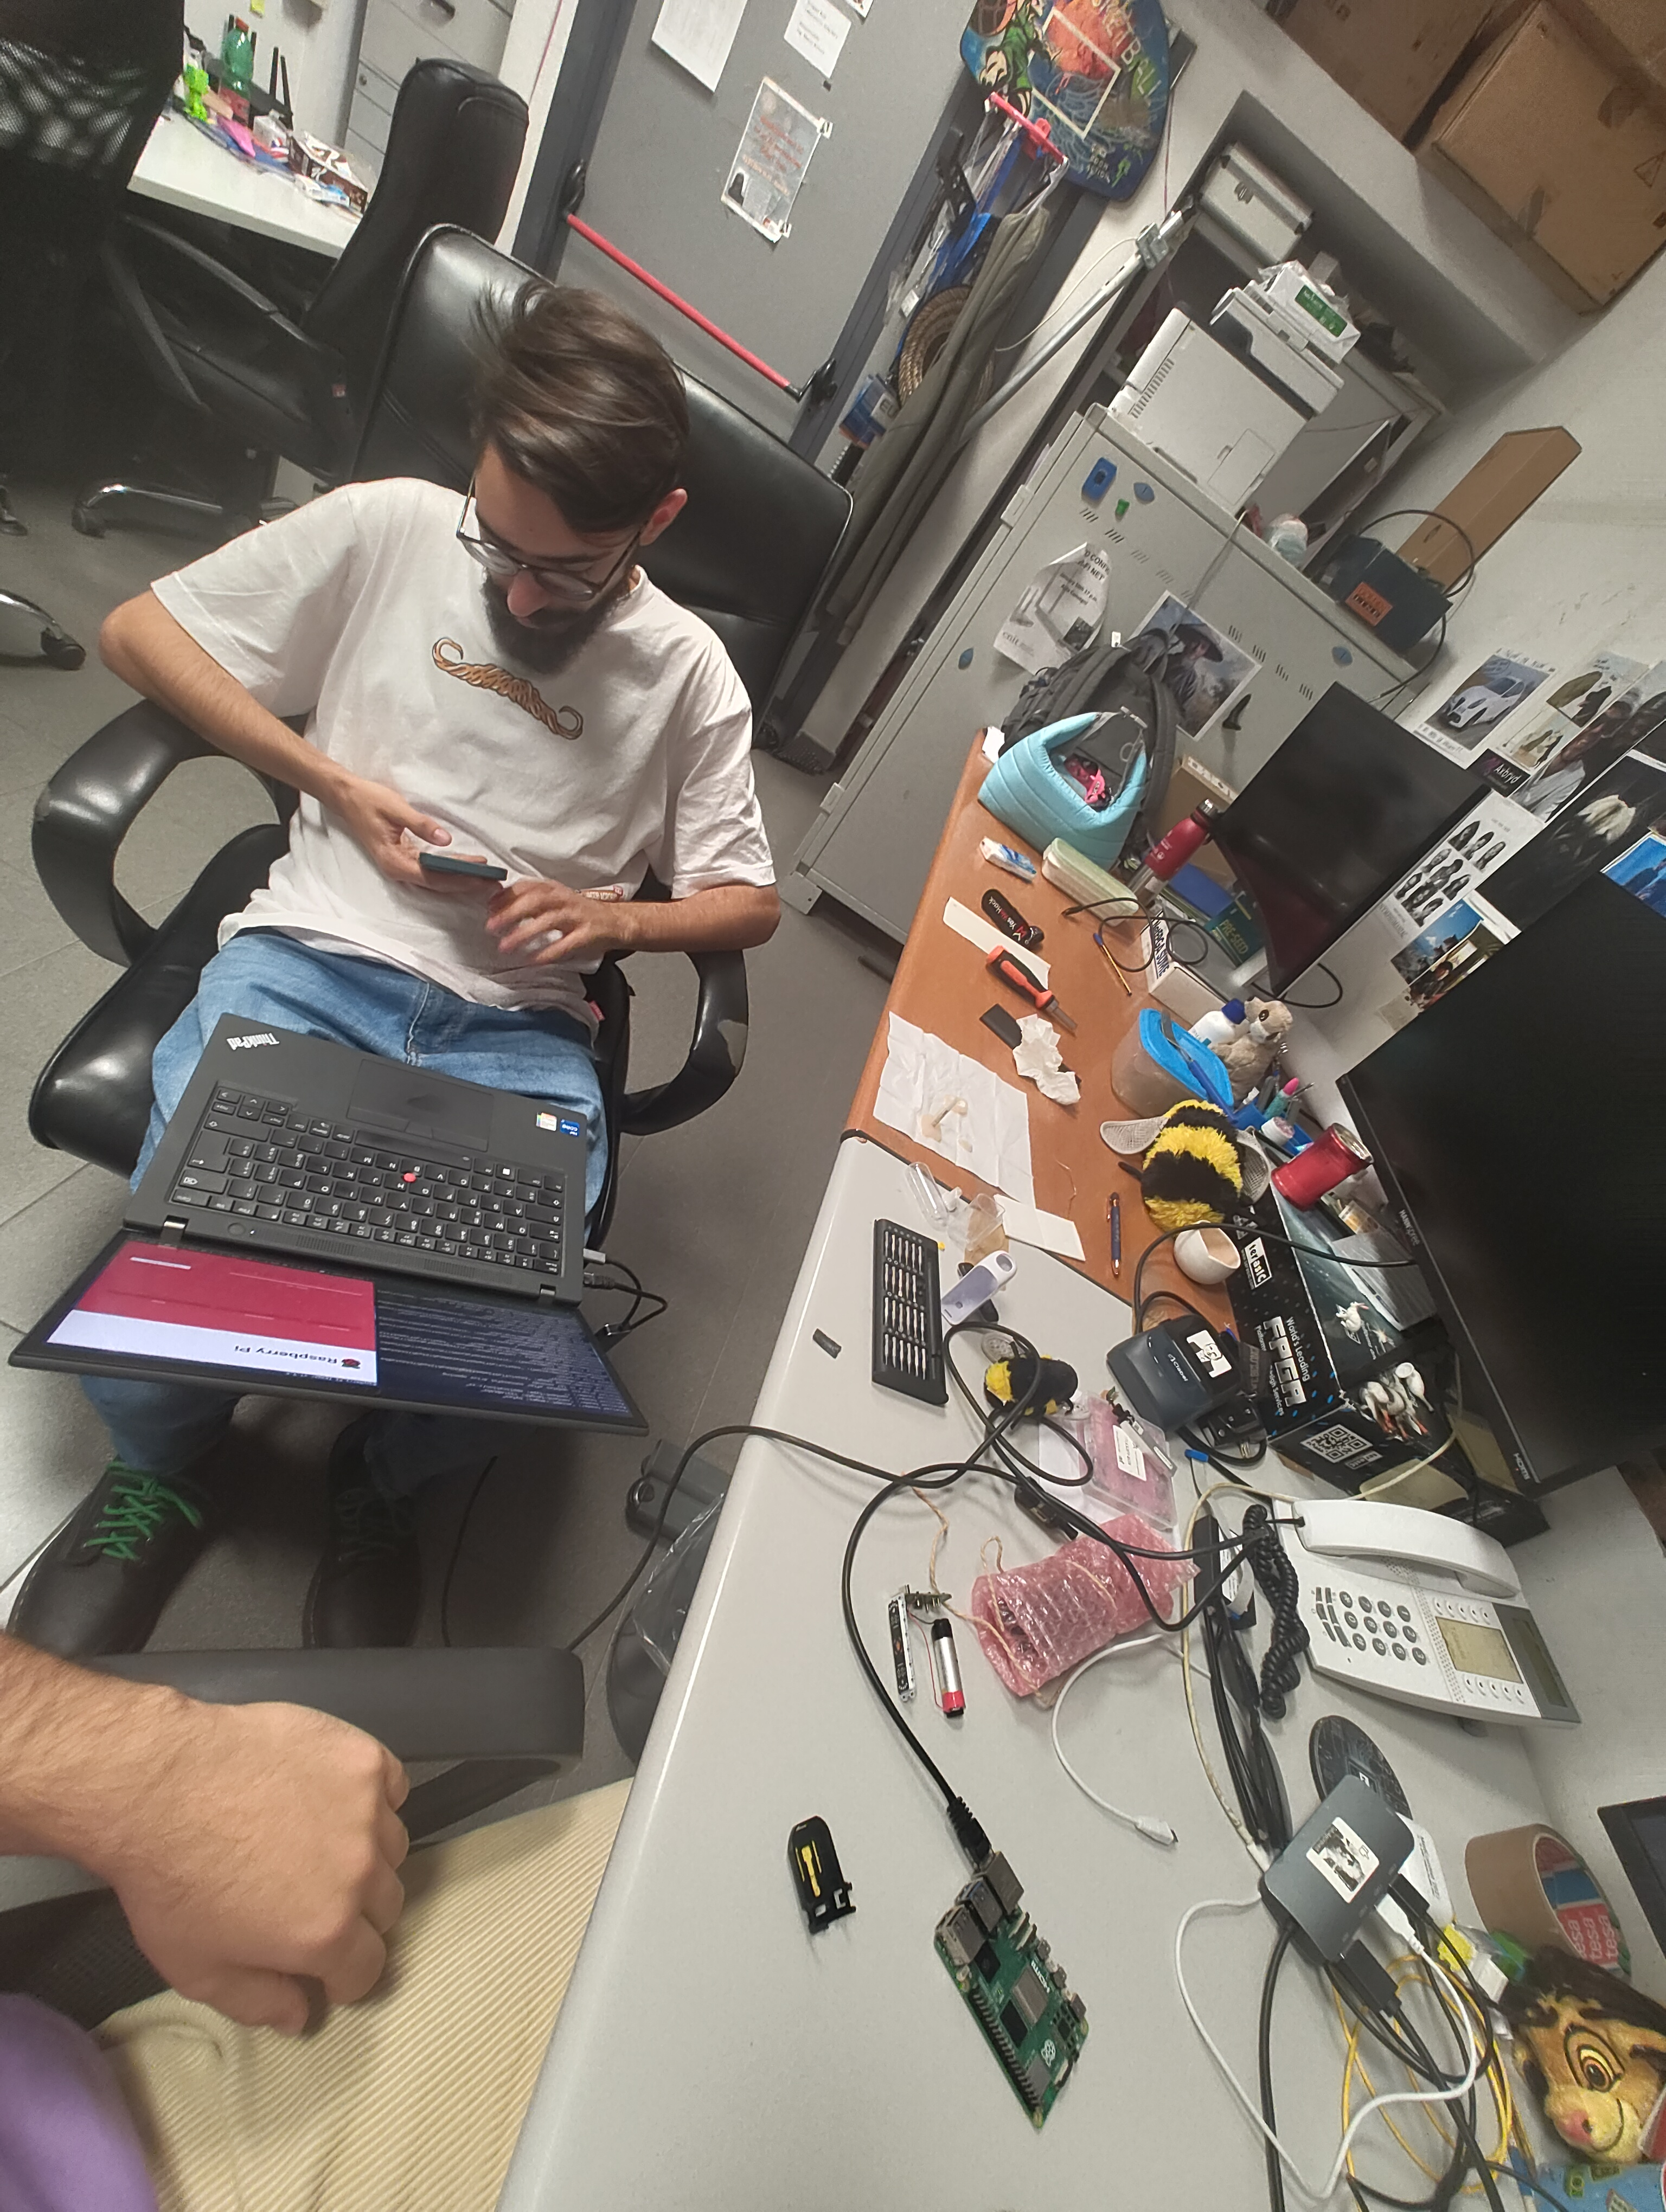
\includegraphics[width=.75\textwidth]{assets/pi5.jpg}
			\end{minipage}
		\end{frame}
	\end{NoHyper}

   \begin{NoHyper}
        \begin{frame}{SWD interaction - first attempt}
			\begin{minipage}[b]{.5\textwidth}
				\begin{itemize}
					\item We encountered problems when compiling \texttt{openocd} (apparently when linking with C math library...)
				\end{itemize}
			\end{minipage}%
			\begin{minipage}[b]{.5\textwidth}
				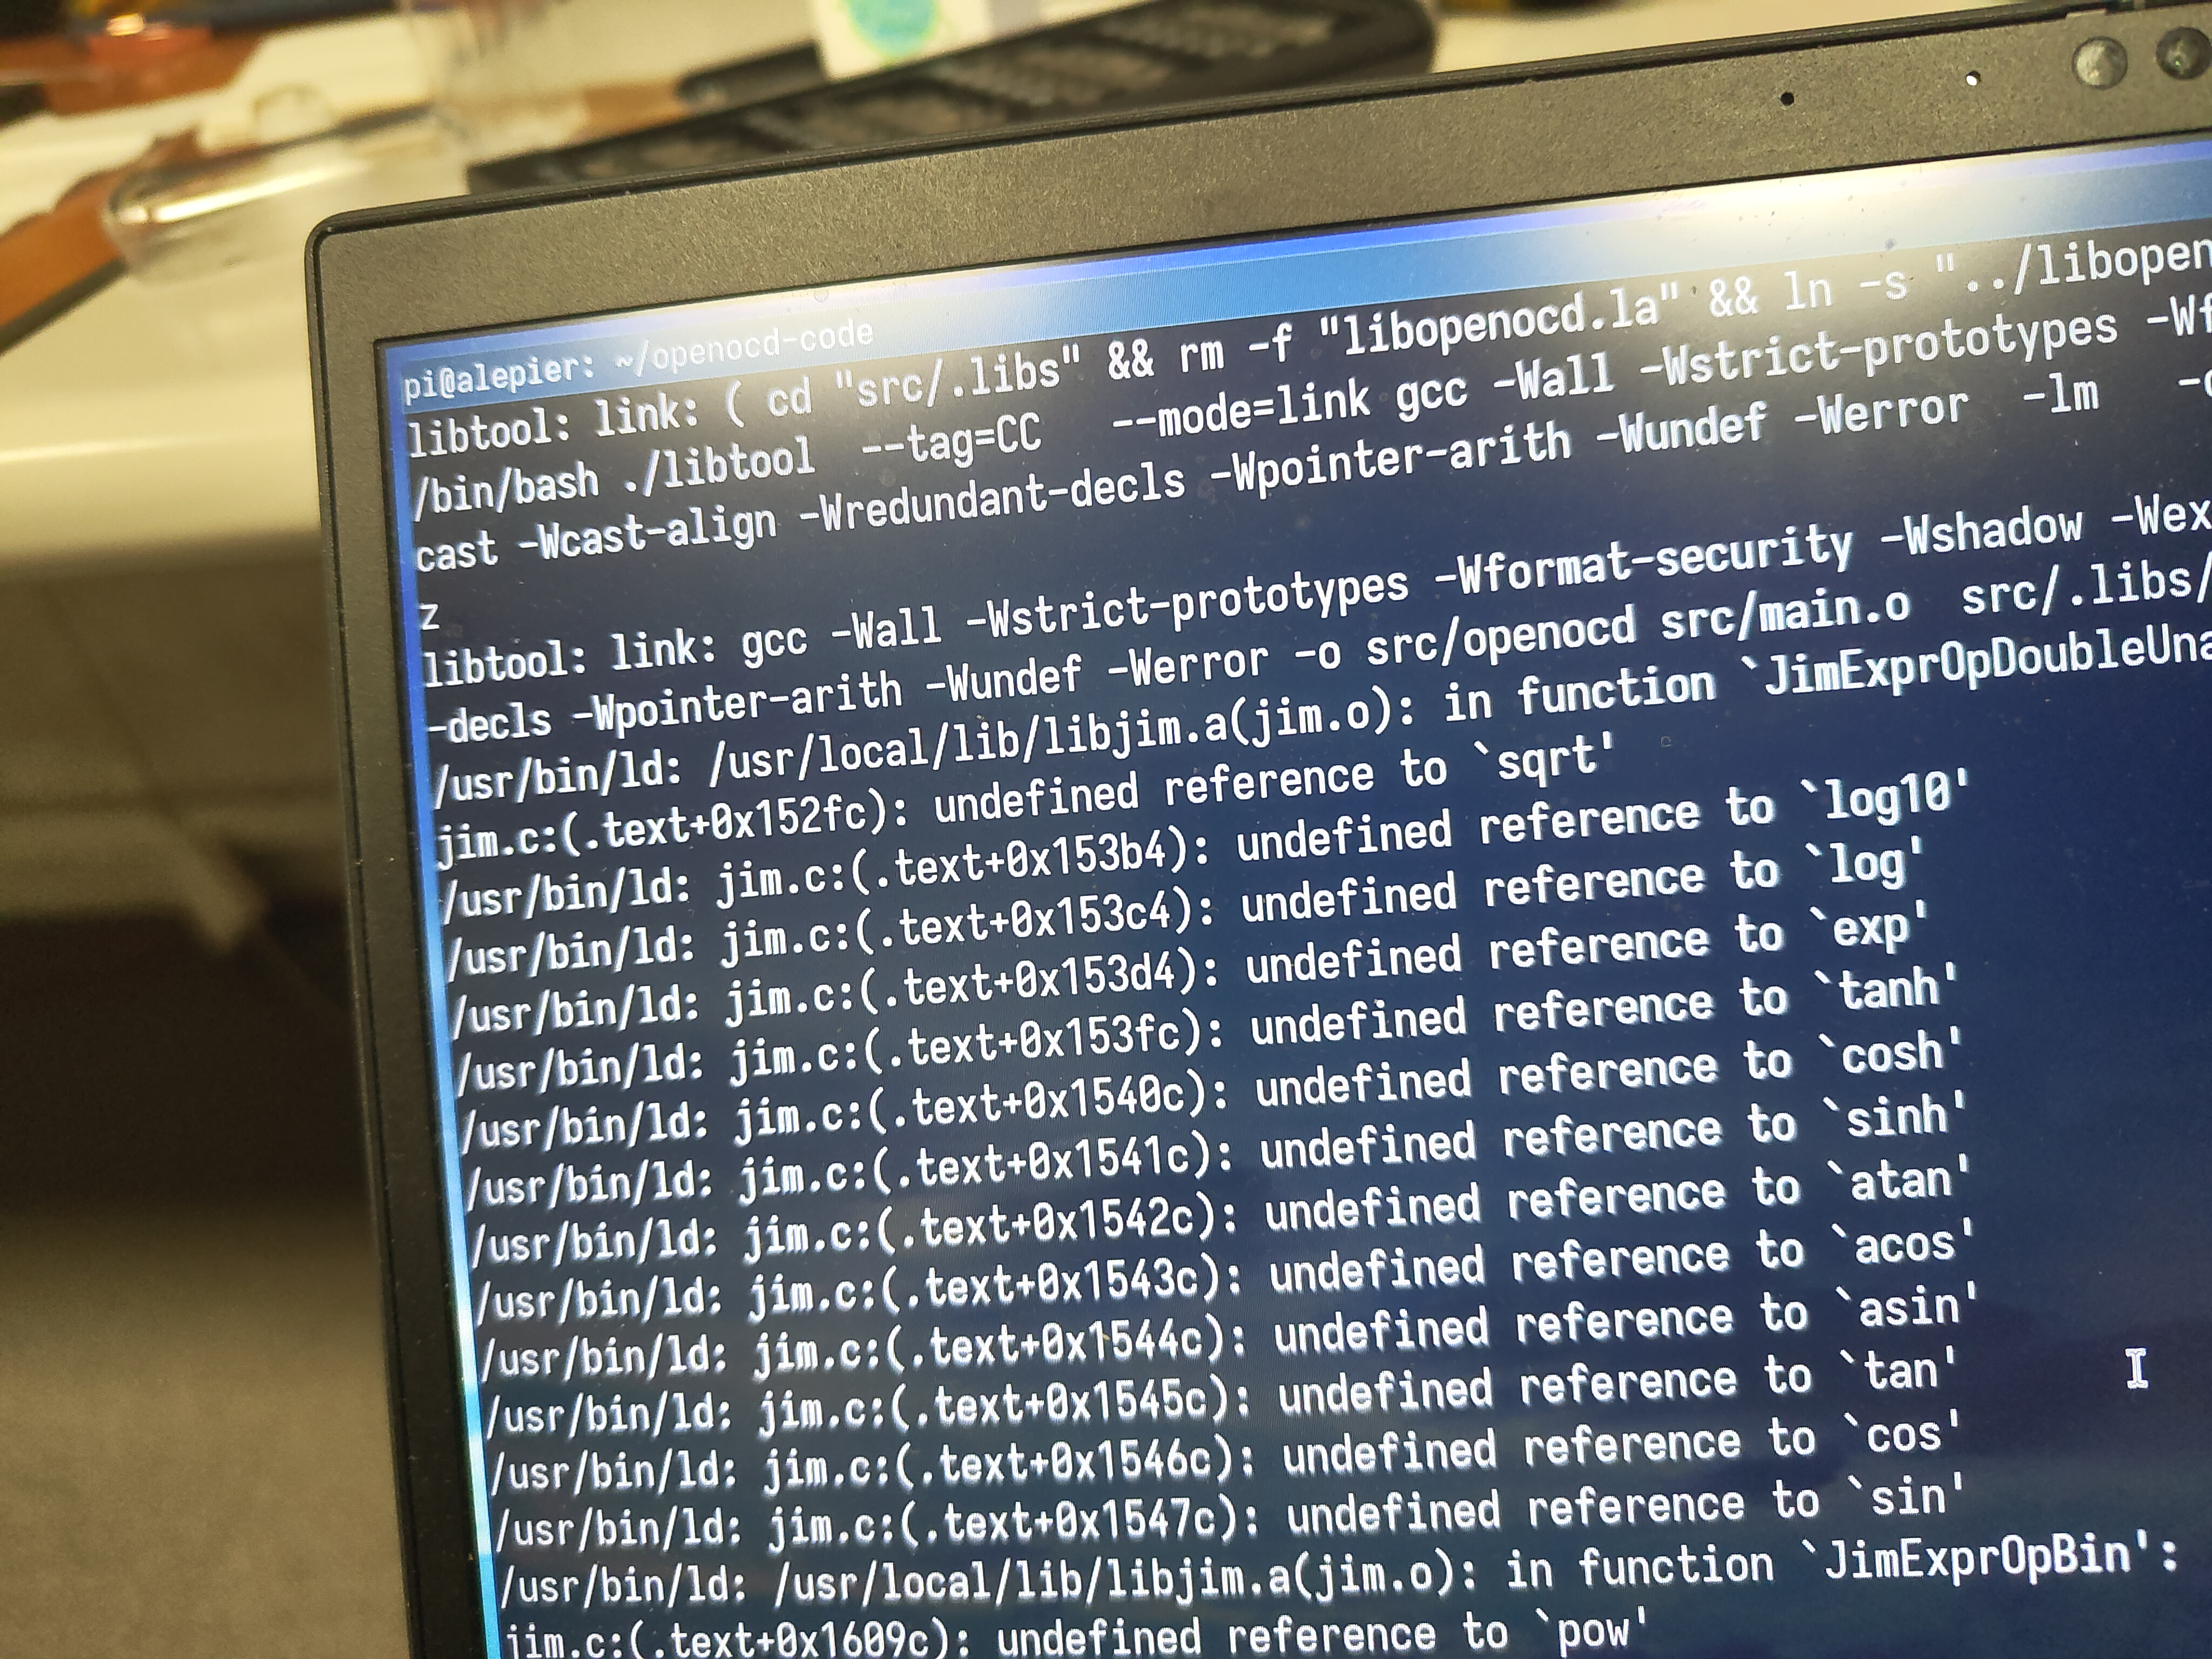
\includegraphics[width=\textwidth]{assets/jim.jpg}
			\end{minipage}
		\end{frame}
	\end{NoHyper}

   \begin{NoHyper}
        \begin{frame}{SWD interaction - first attempt}
			\begin{minipage}[b]{.5\textwidth}
				\begin{itemize}
					\item By looking at Pi5 pinout it seemed like we could interact with SWD...
				\end{itemize}
			\end{minipage}%
			\begin{minipage}[b]{.5\textwidth}
				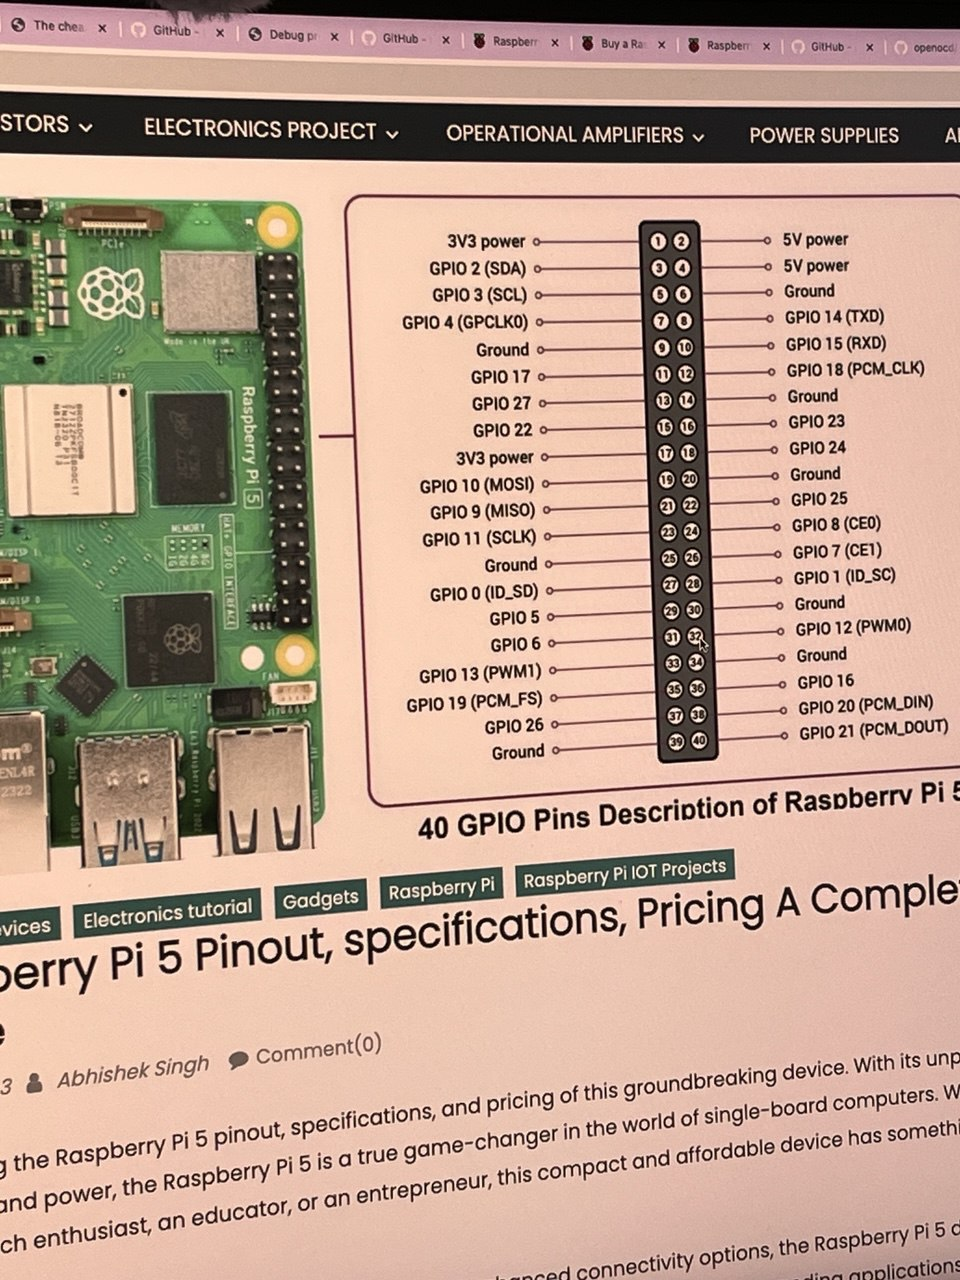
\includegraphics[width=.8\textwidth]{assets/pi5_pinout.jpg}
			\end{minipage}
		\end{frame}
	\end{NoHyper}

   \begin{NoHyper}
			\section{Atto II}
			\frame{\sectionpage}
	\end{NoHyper}

   \begin{NoHyper}
        \begin{frame}{Let's buy some stuff}
			\begin{minipage}[b]{.5\textwidth}
			\begin{itemize}
				\item We decided to buy some tools that would help our SWD probing
				\item Essentially, we needed a Jlink, but we were not sure about which one to use
			\end{itemize}
			\end{minipage}%
			\begin{minipage}[b]{.5\textwidth}
				\begin{flushright}
					\centering
					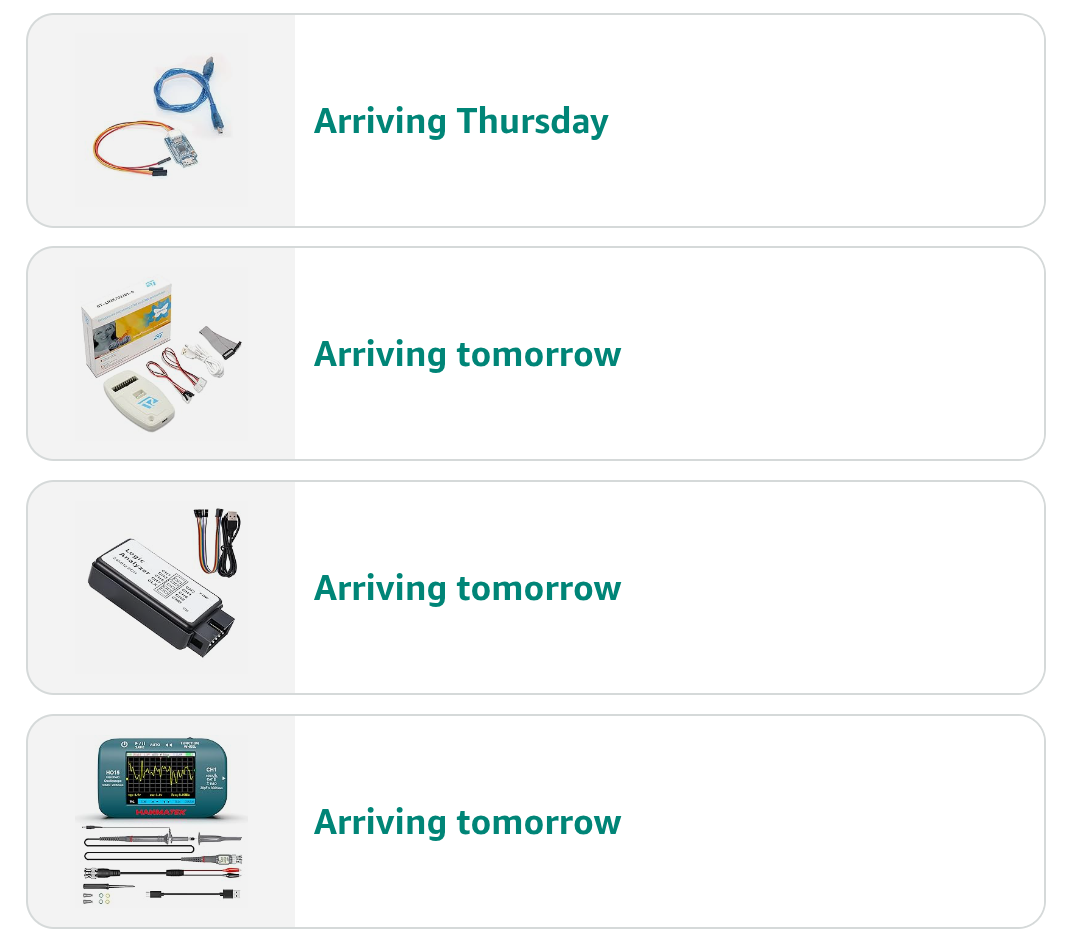
\includegraphics[width=.9\textwidth]{assets/acquisti}
  				\end{flushright}
			\end{minipage}
		\end{frame}
	\end{NoHyper}

   \begin{NoHyper}
        \begin{frame}{SWD pinout hunt}
			\begin{figure}
				\centering
				\includegraphics[width=.9\textwidth]{assets/setup_one}
			\end{figure}
		\end{frame}
	\end{NoHyper}

   \begin{NoHyper}
        \begin{frame}{SWD pinout hunt}
			Got our 9V legacy battery to power out multimeter and start hunting for SWD pins
			\begin{figure}[t!]
				\subfloat{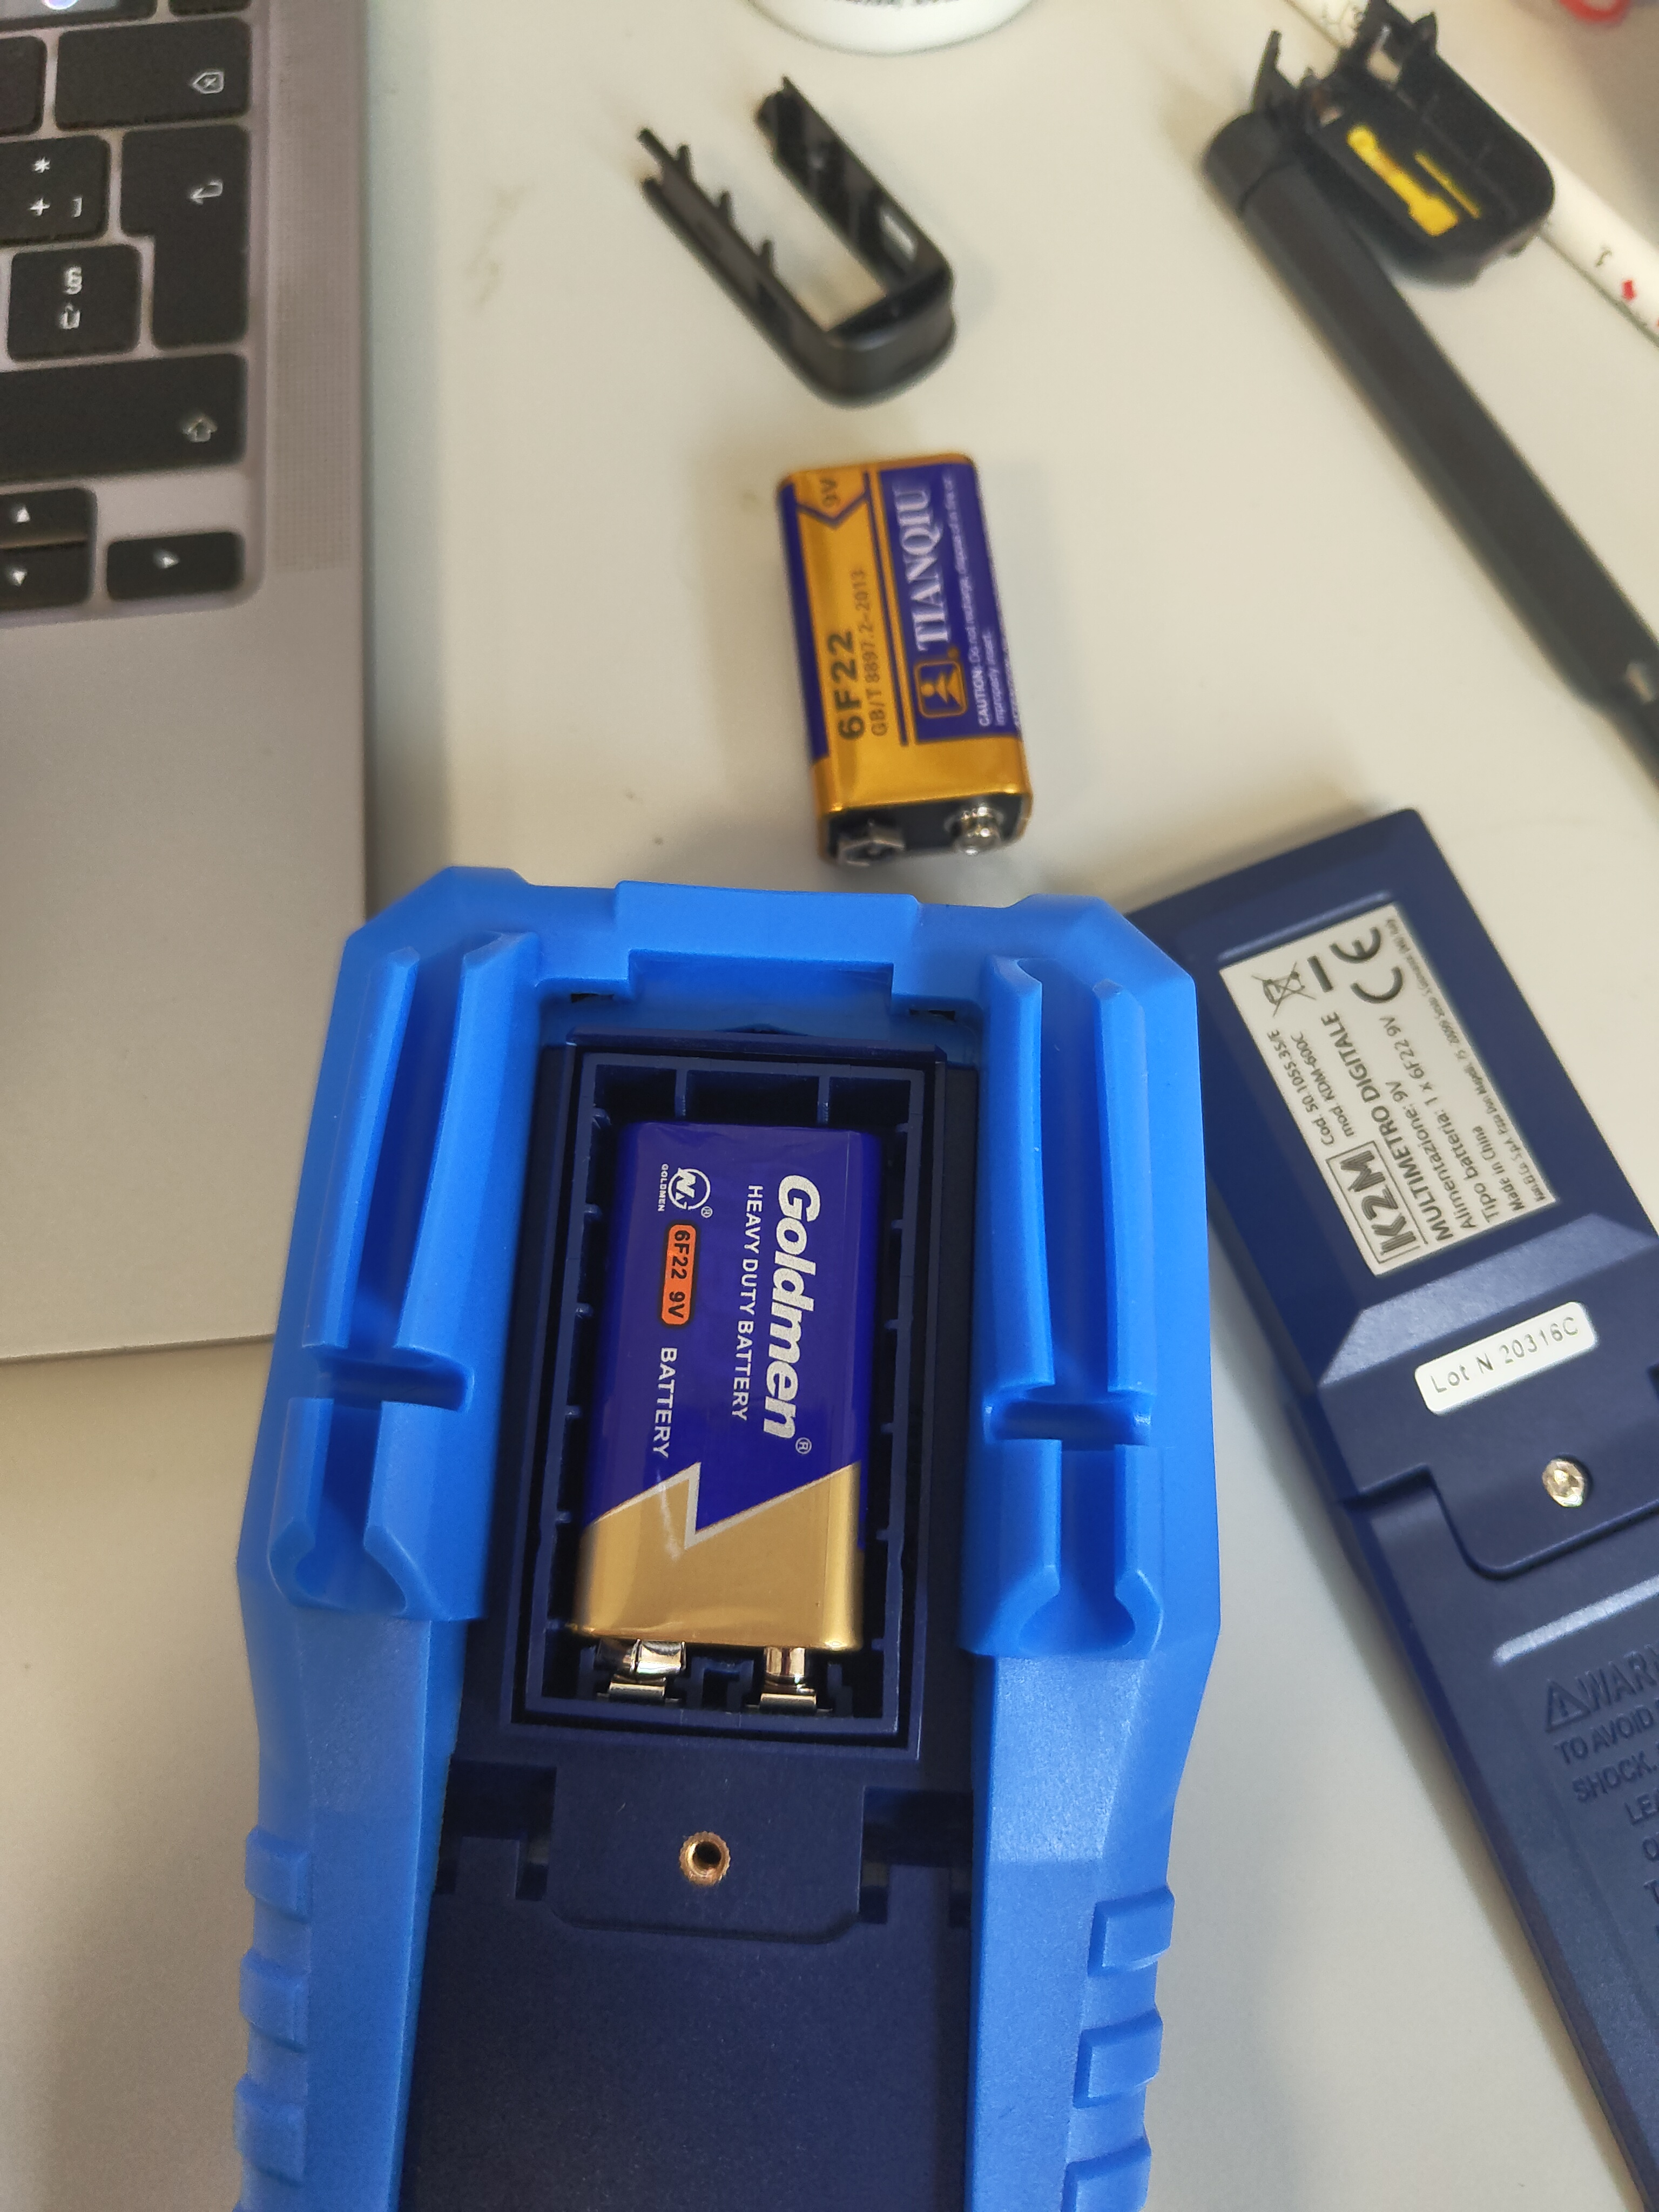
\includegraphics[width=0.3\linewidth]{assets/multimeter.jpg}}\hfill
  				\subfloat{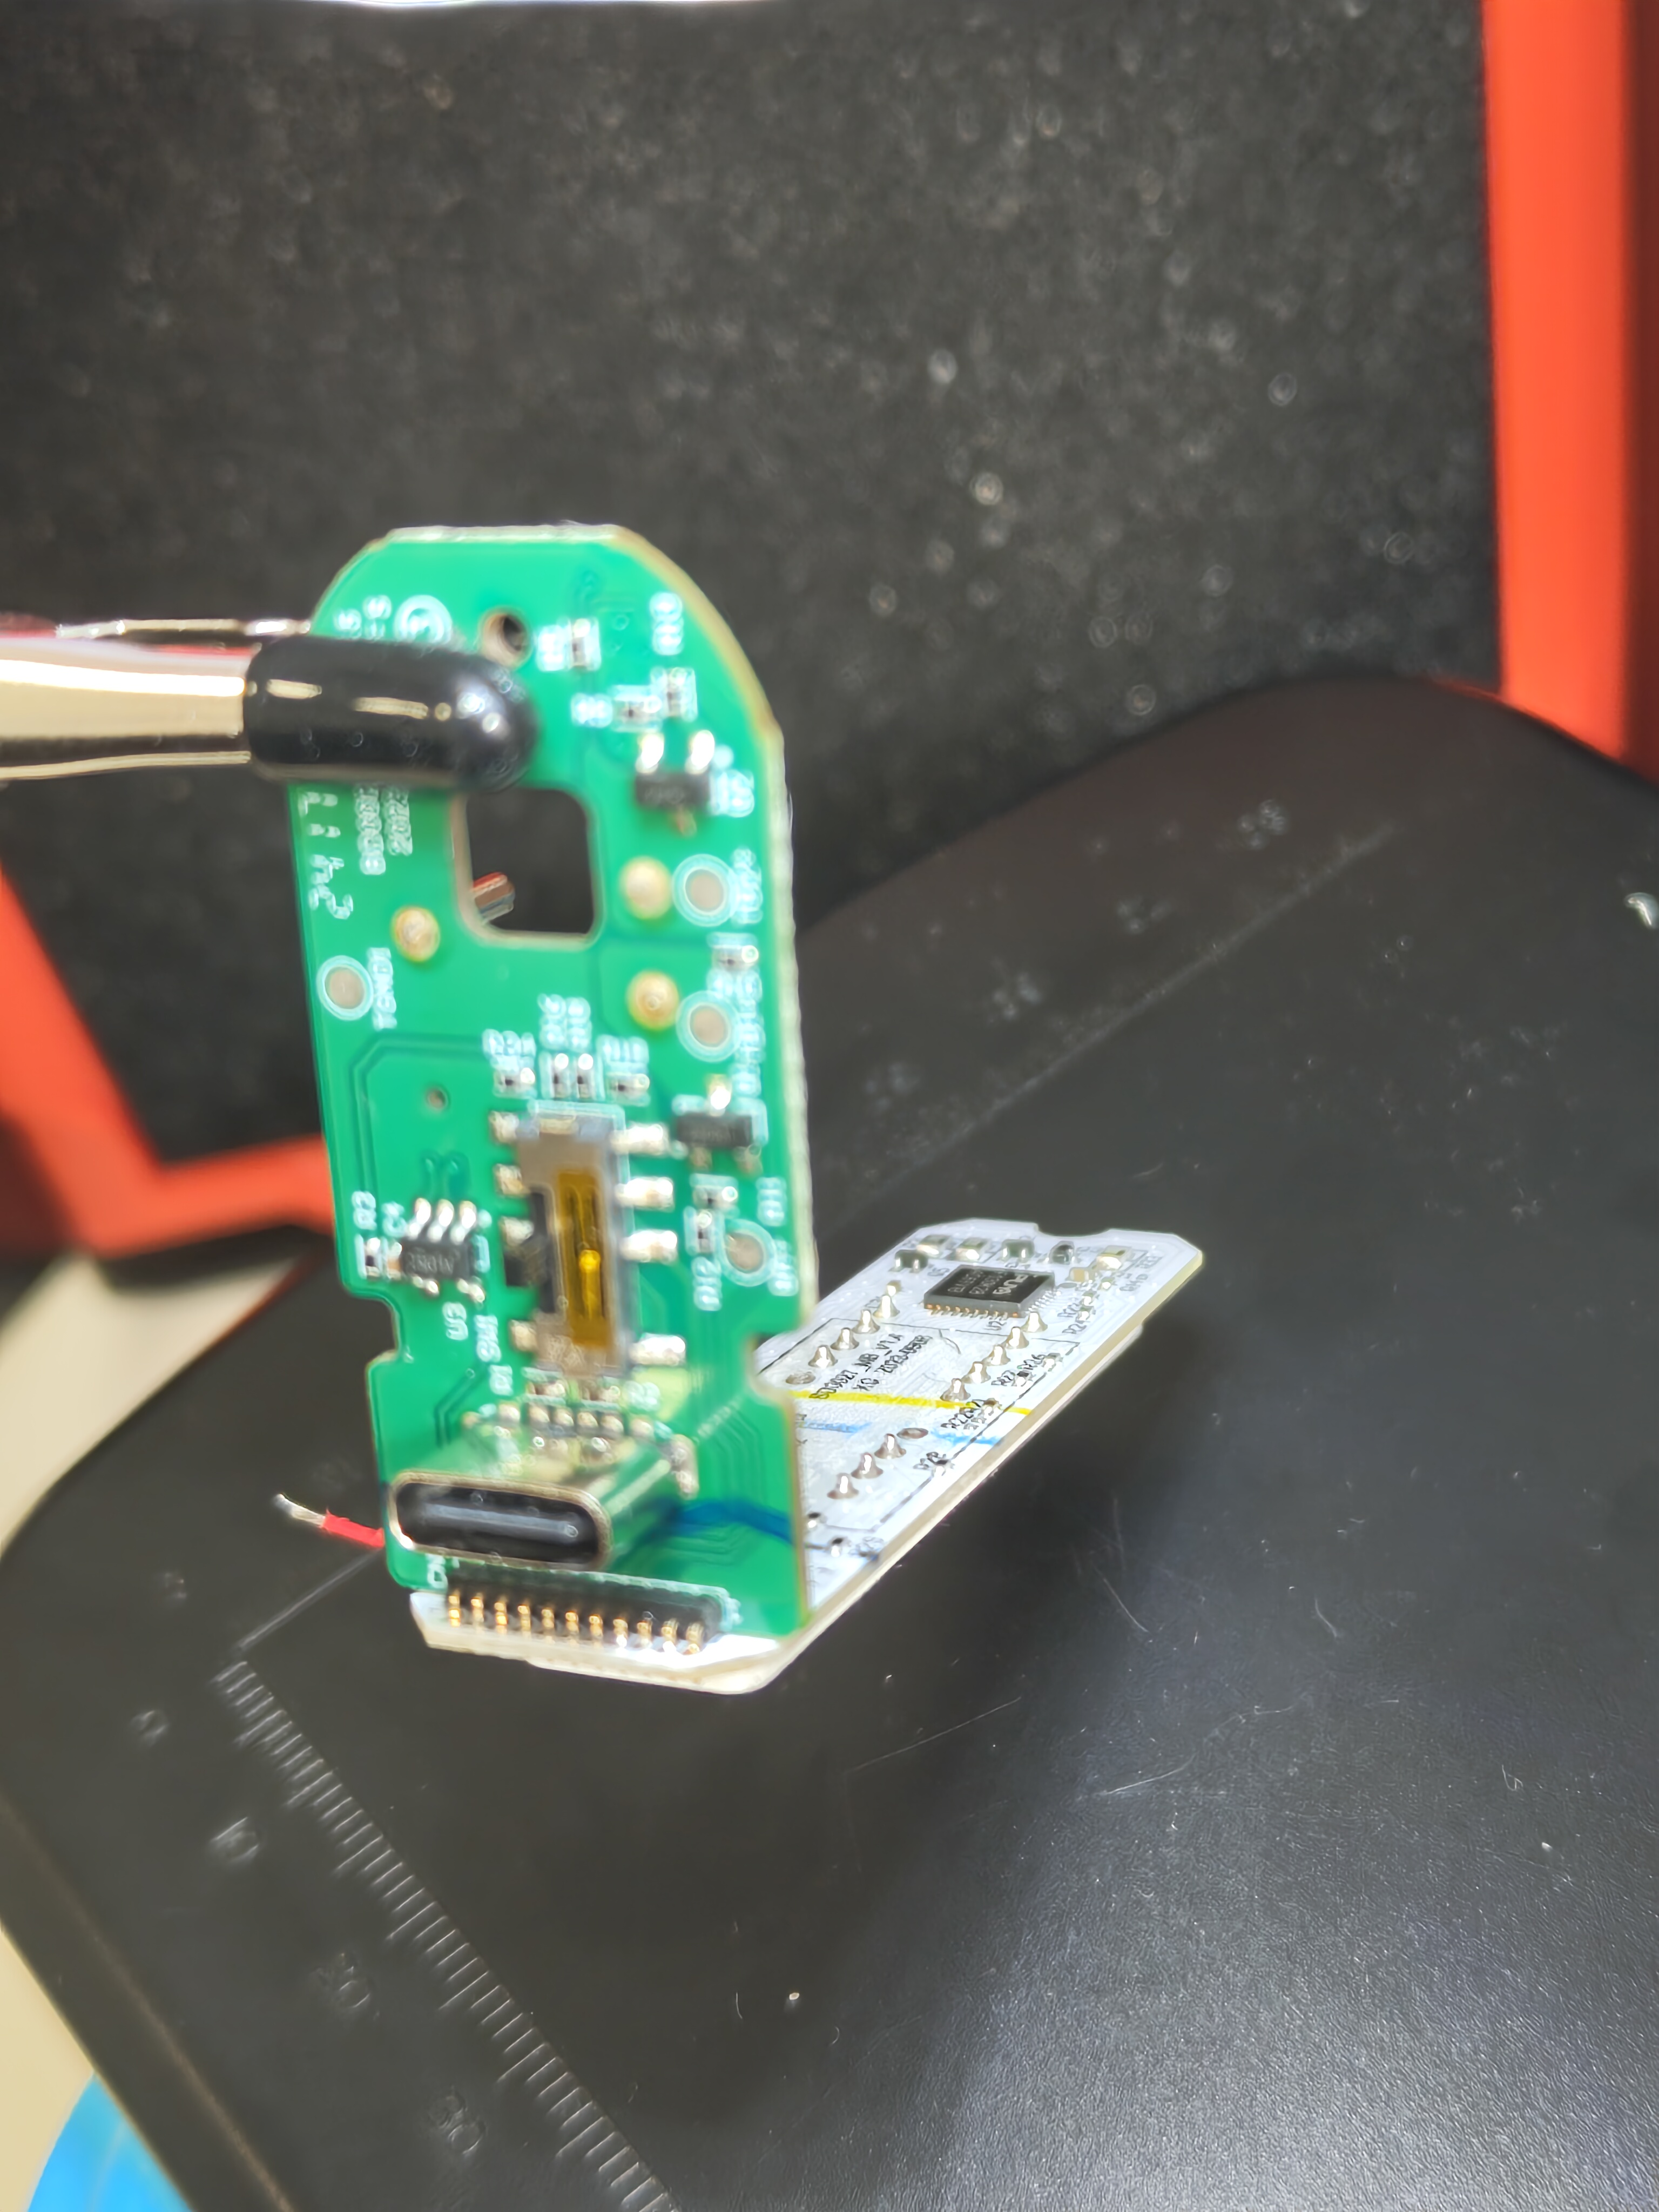
\includegraphics[width=0.3\linewidth]{assets/pcb_1_2.jpg}}\hfill
  				\subfloat{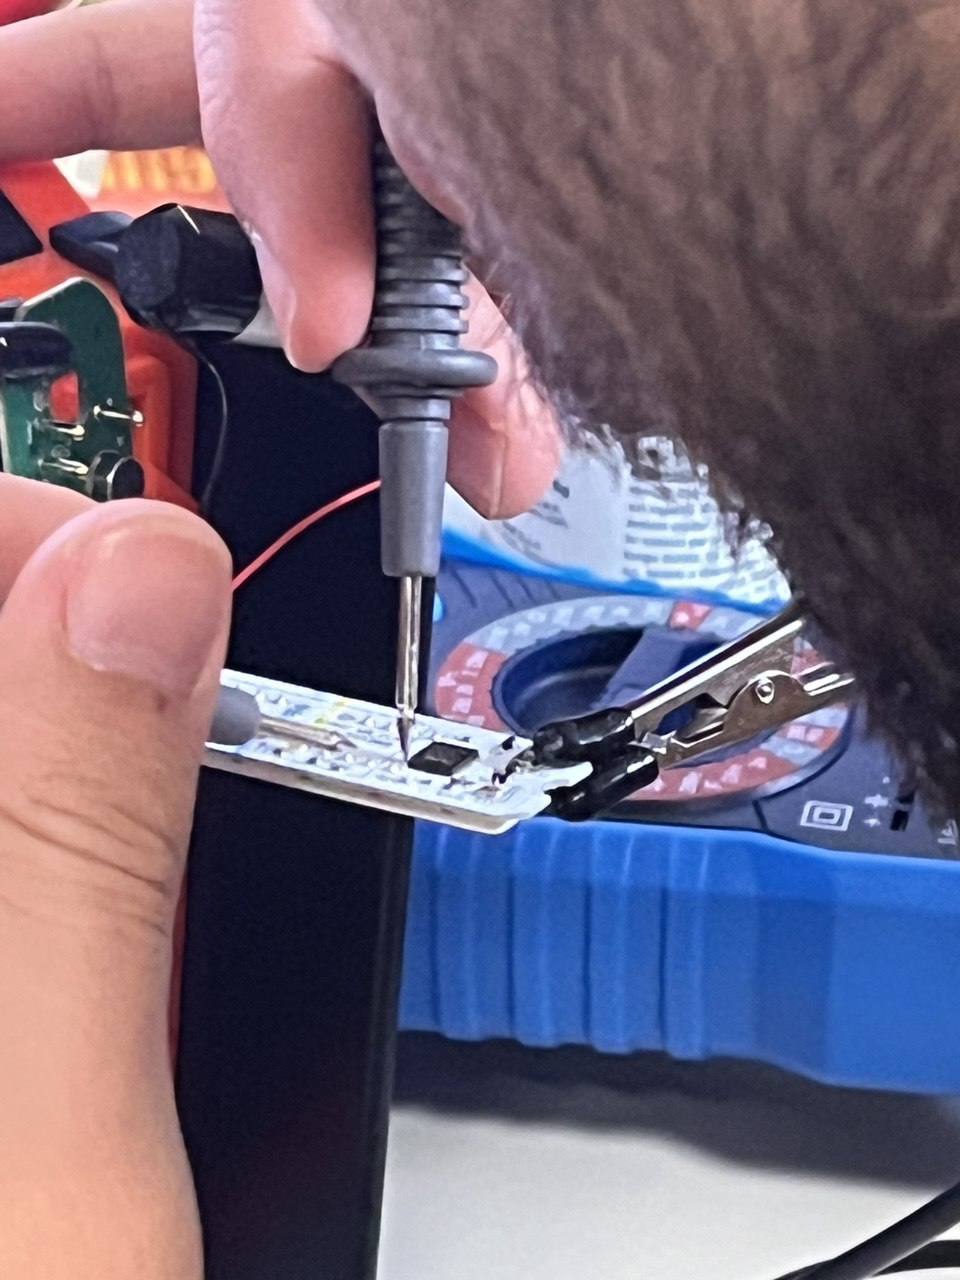
\includegraphics[width=0.3\linewidth]{assets/probe.jpg}}\hfill%
			\end{figure}
		\end{frame}
	\end{NoHyper}

   \begin{NoHyper}
        \begin{frame}{SWD pinout hunt}
			\begin{minipage}[b]{.5\textwidth}
				\begin{itemize}
					\item We probed around with the multimeter to find out the SWD pinout position and weather it was connect somewhere (ideally, USBC)
				\end{itemize}
			\end{minipage}%
			\begin{minipage}[b]{.5\textwidth}
				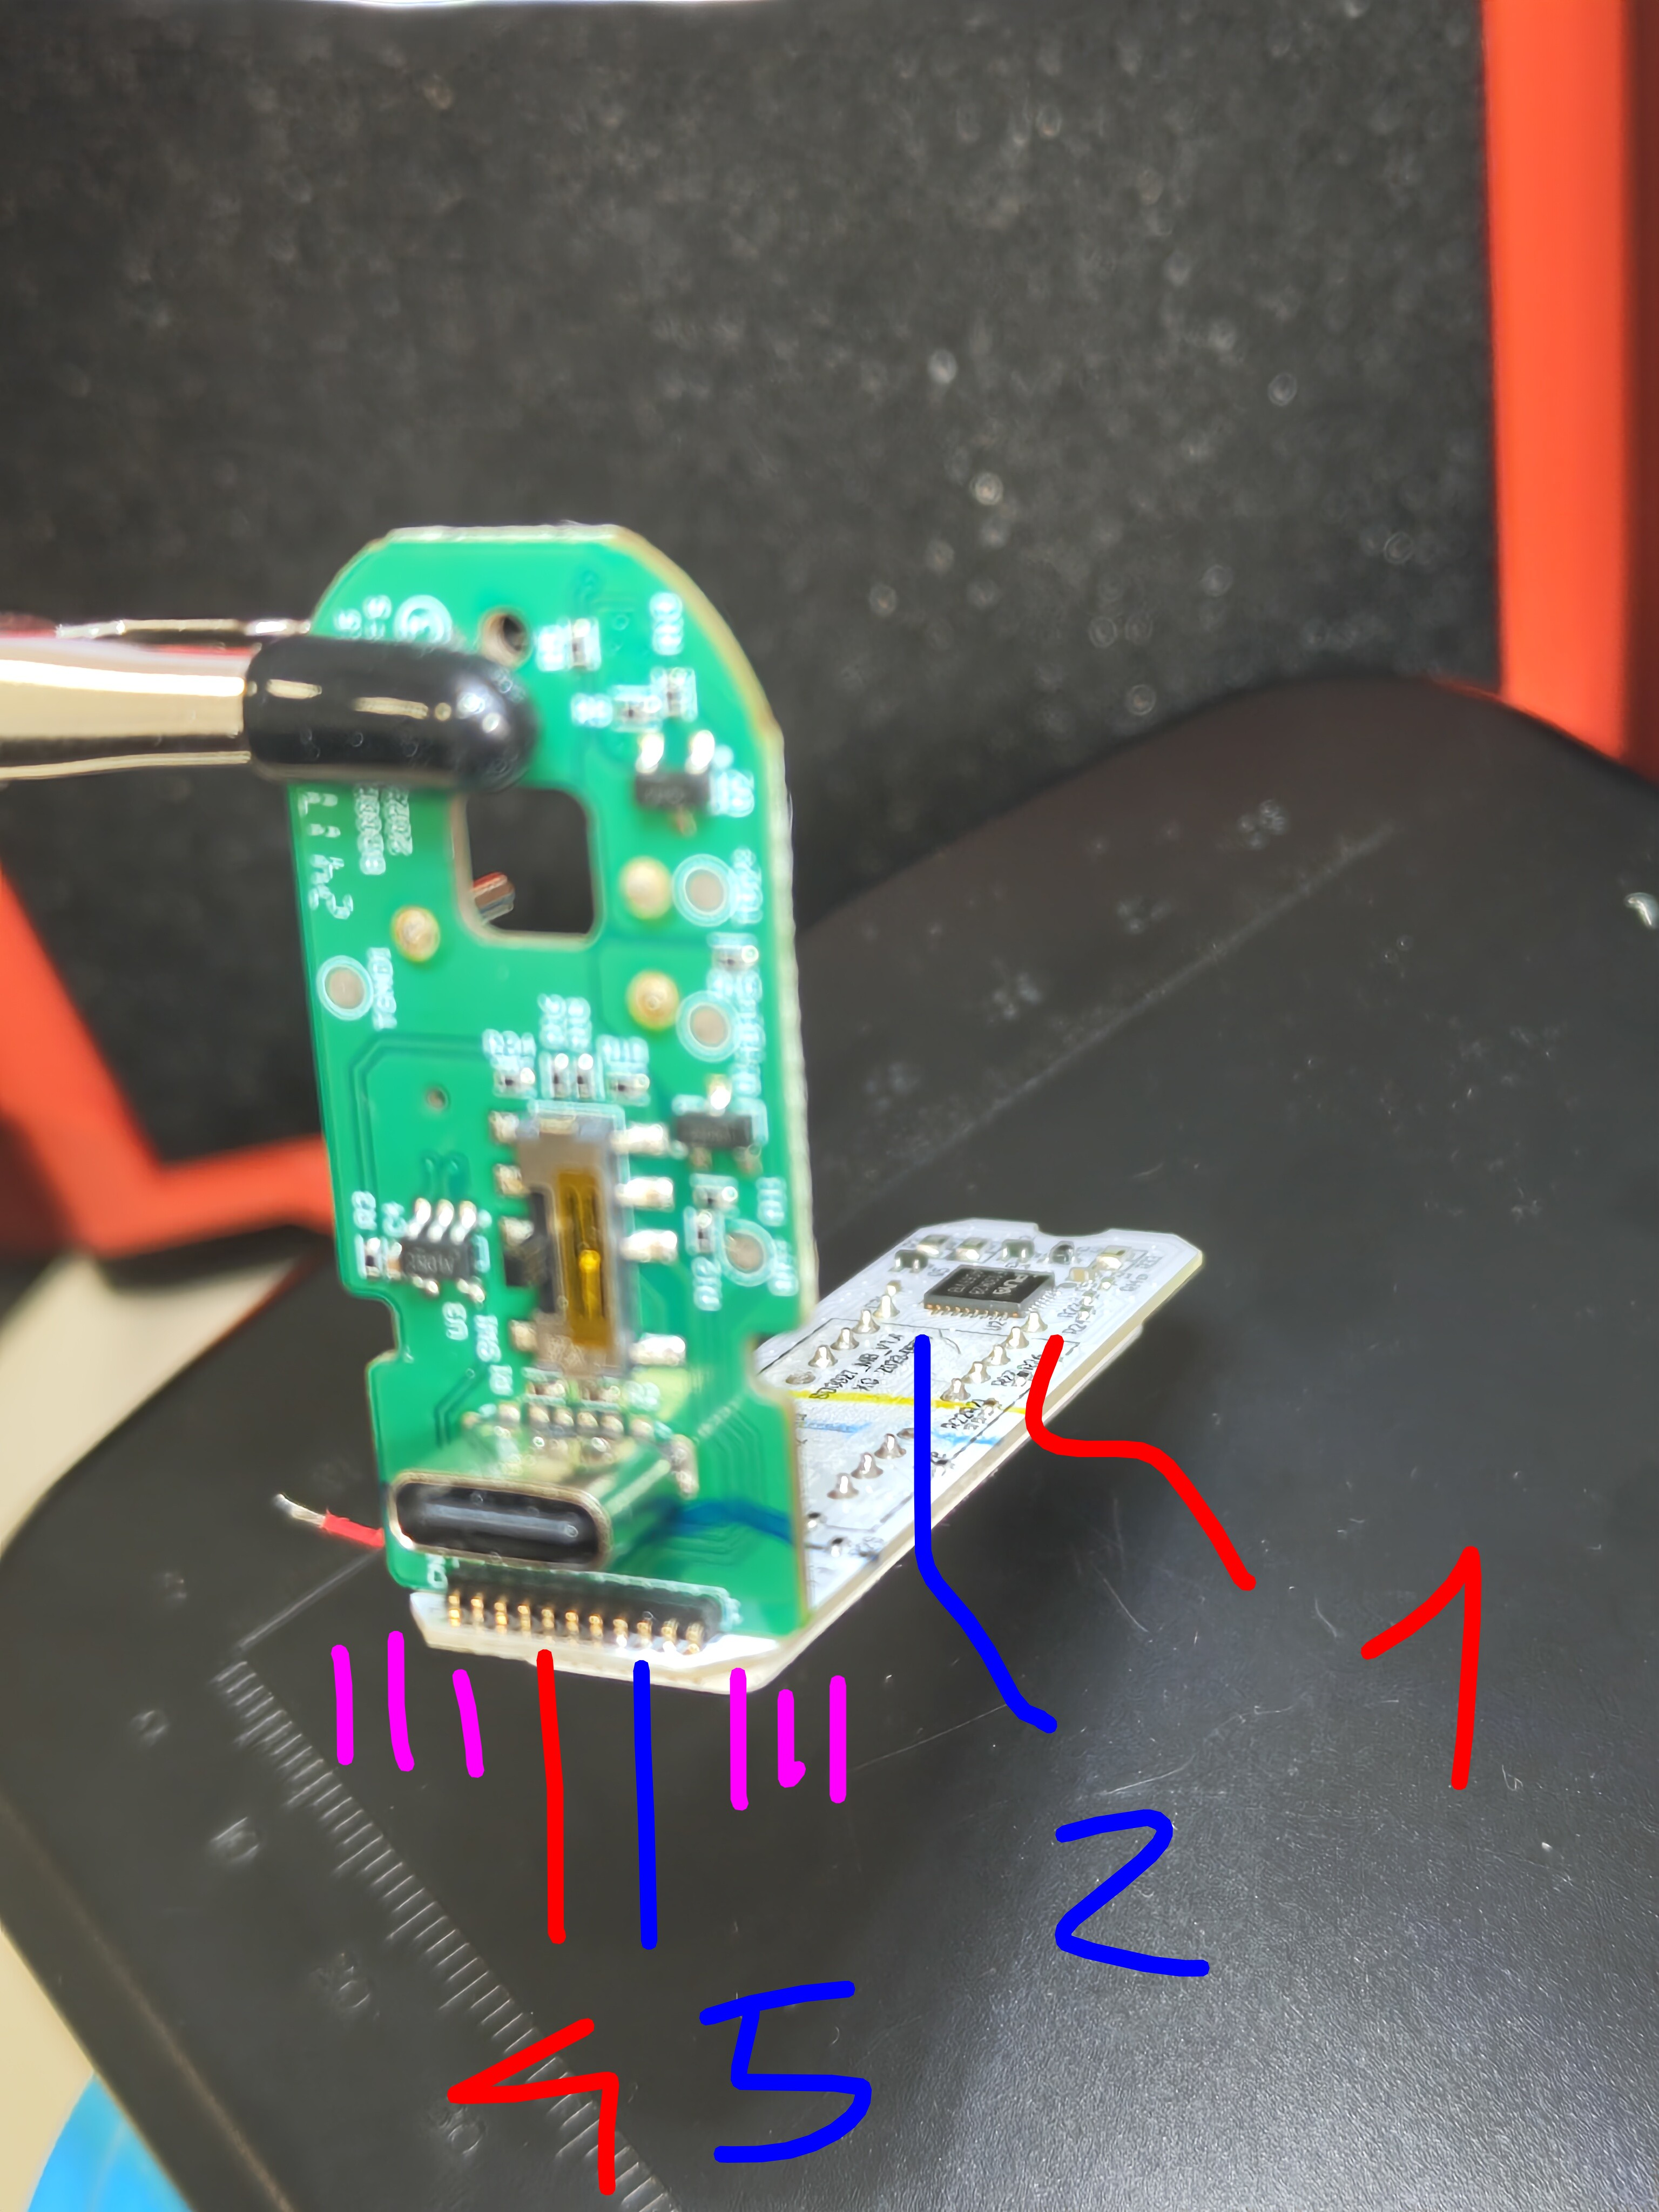
\includegraphics[width=.7\textwidth]{assets/pcb_1.jpg}
			\end{minipage}
		\end{frame}
	\end{NoHyper}

   \begin{NoHyper}
        \begin{frame}{Setup details}
			\begin{figure}
				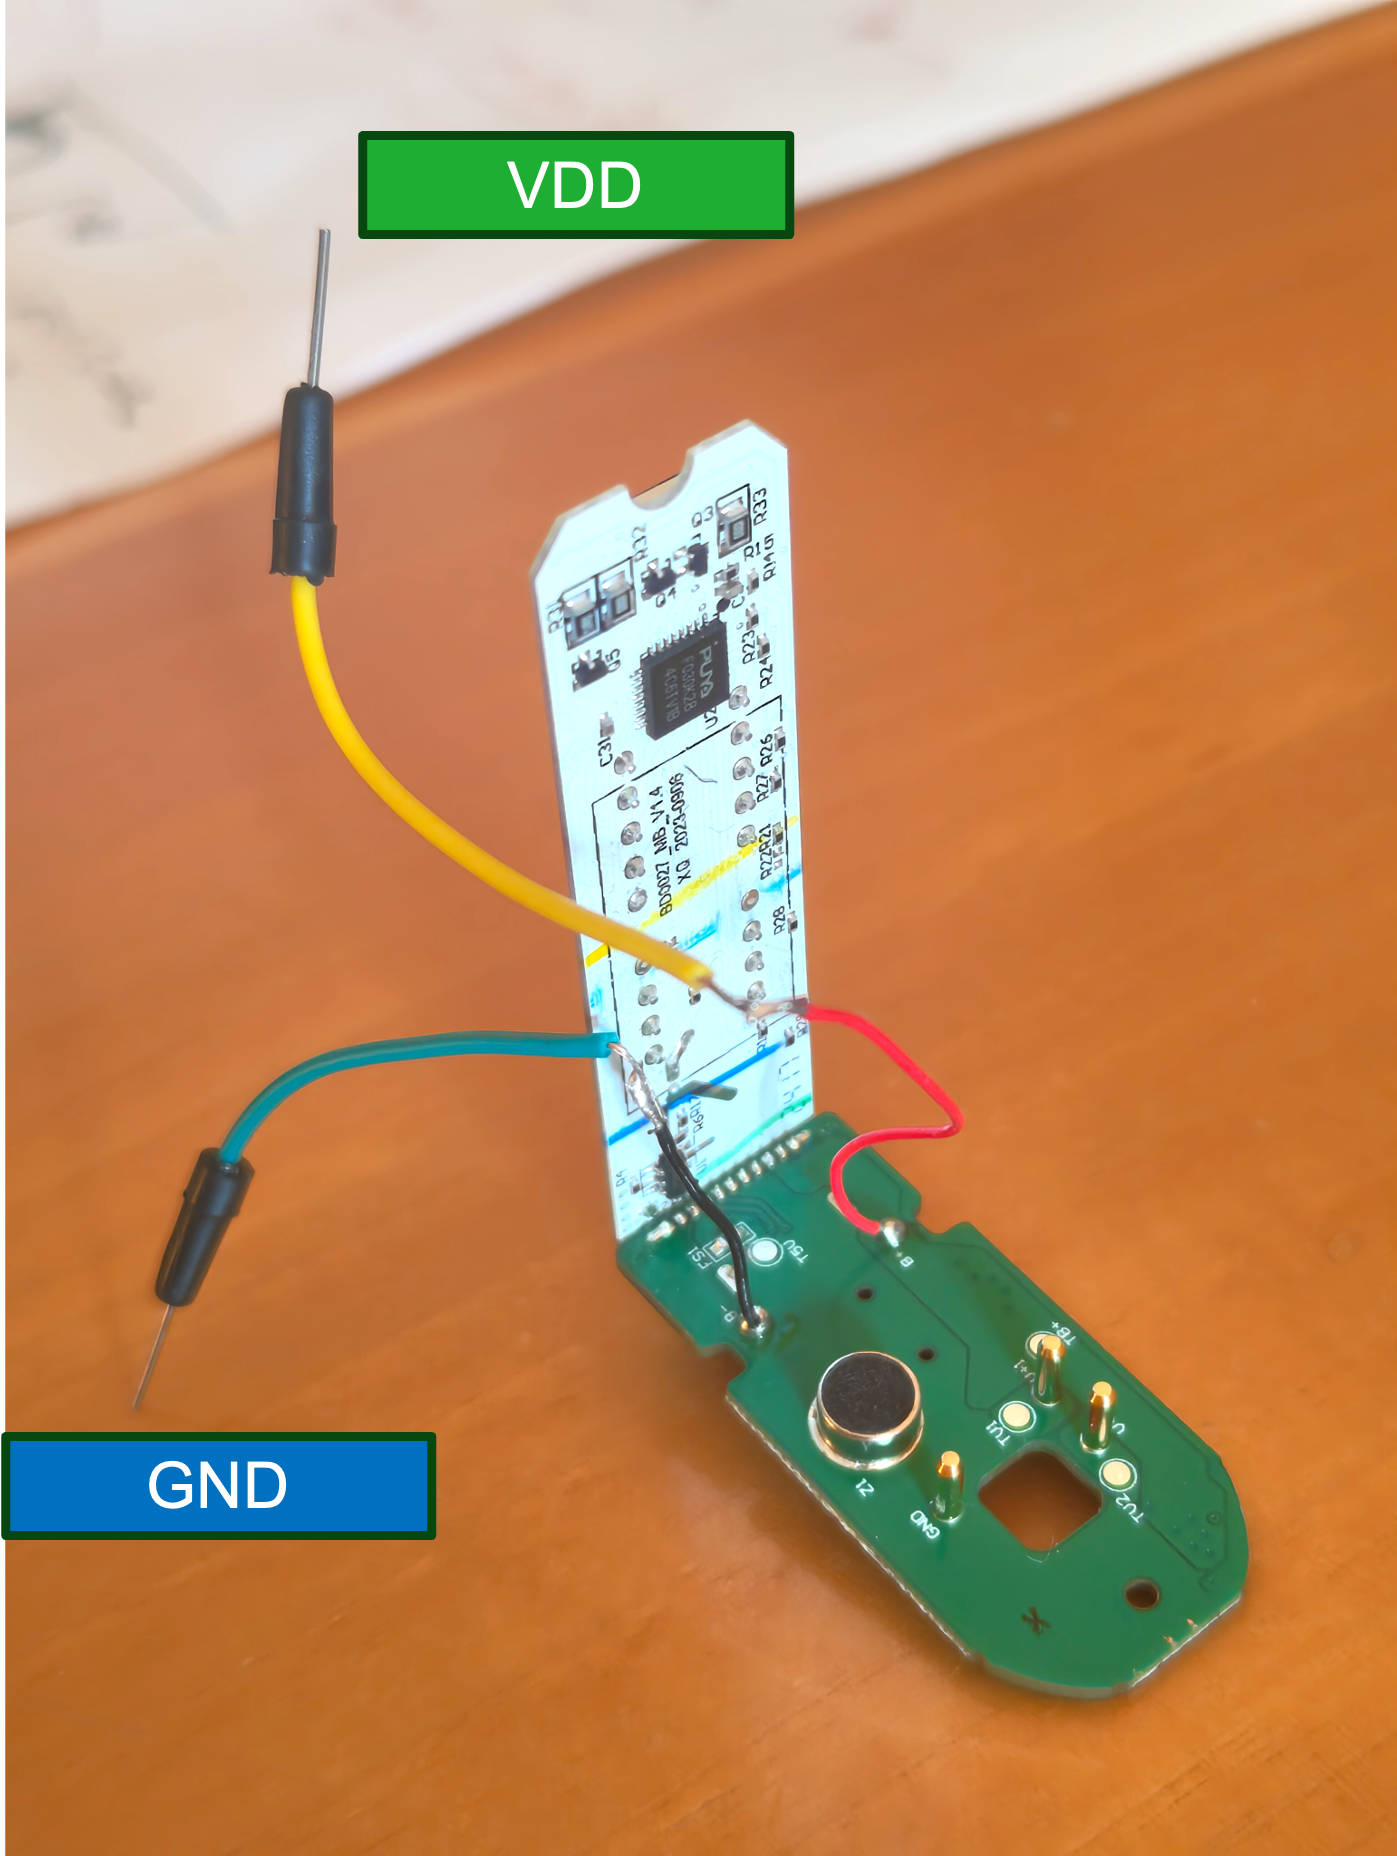
\includegraphics[width=.45\textwidth]{assets/board_1}
			\end{figure}
		\end{frame}
	\end{NoHyper}

   \begin{NoHyper}
        \begin{frame}{Setup details}
			\begin{figure}
				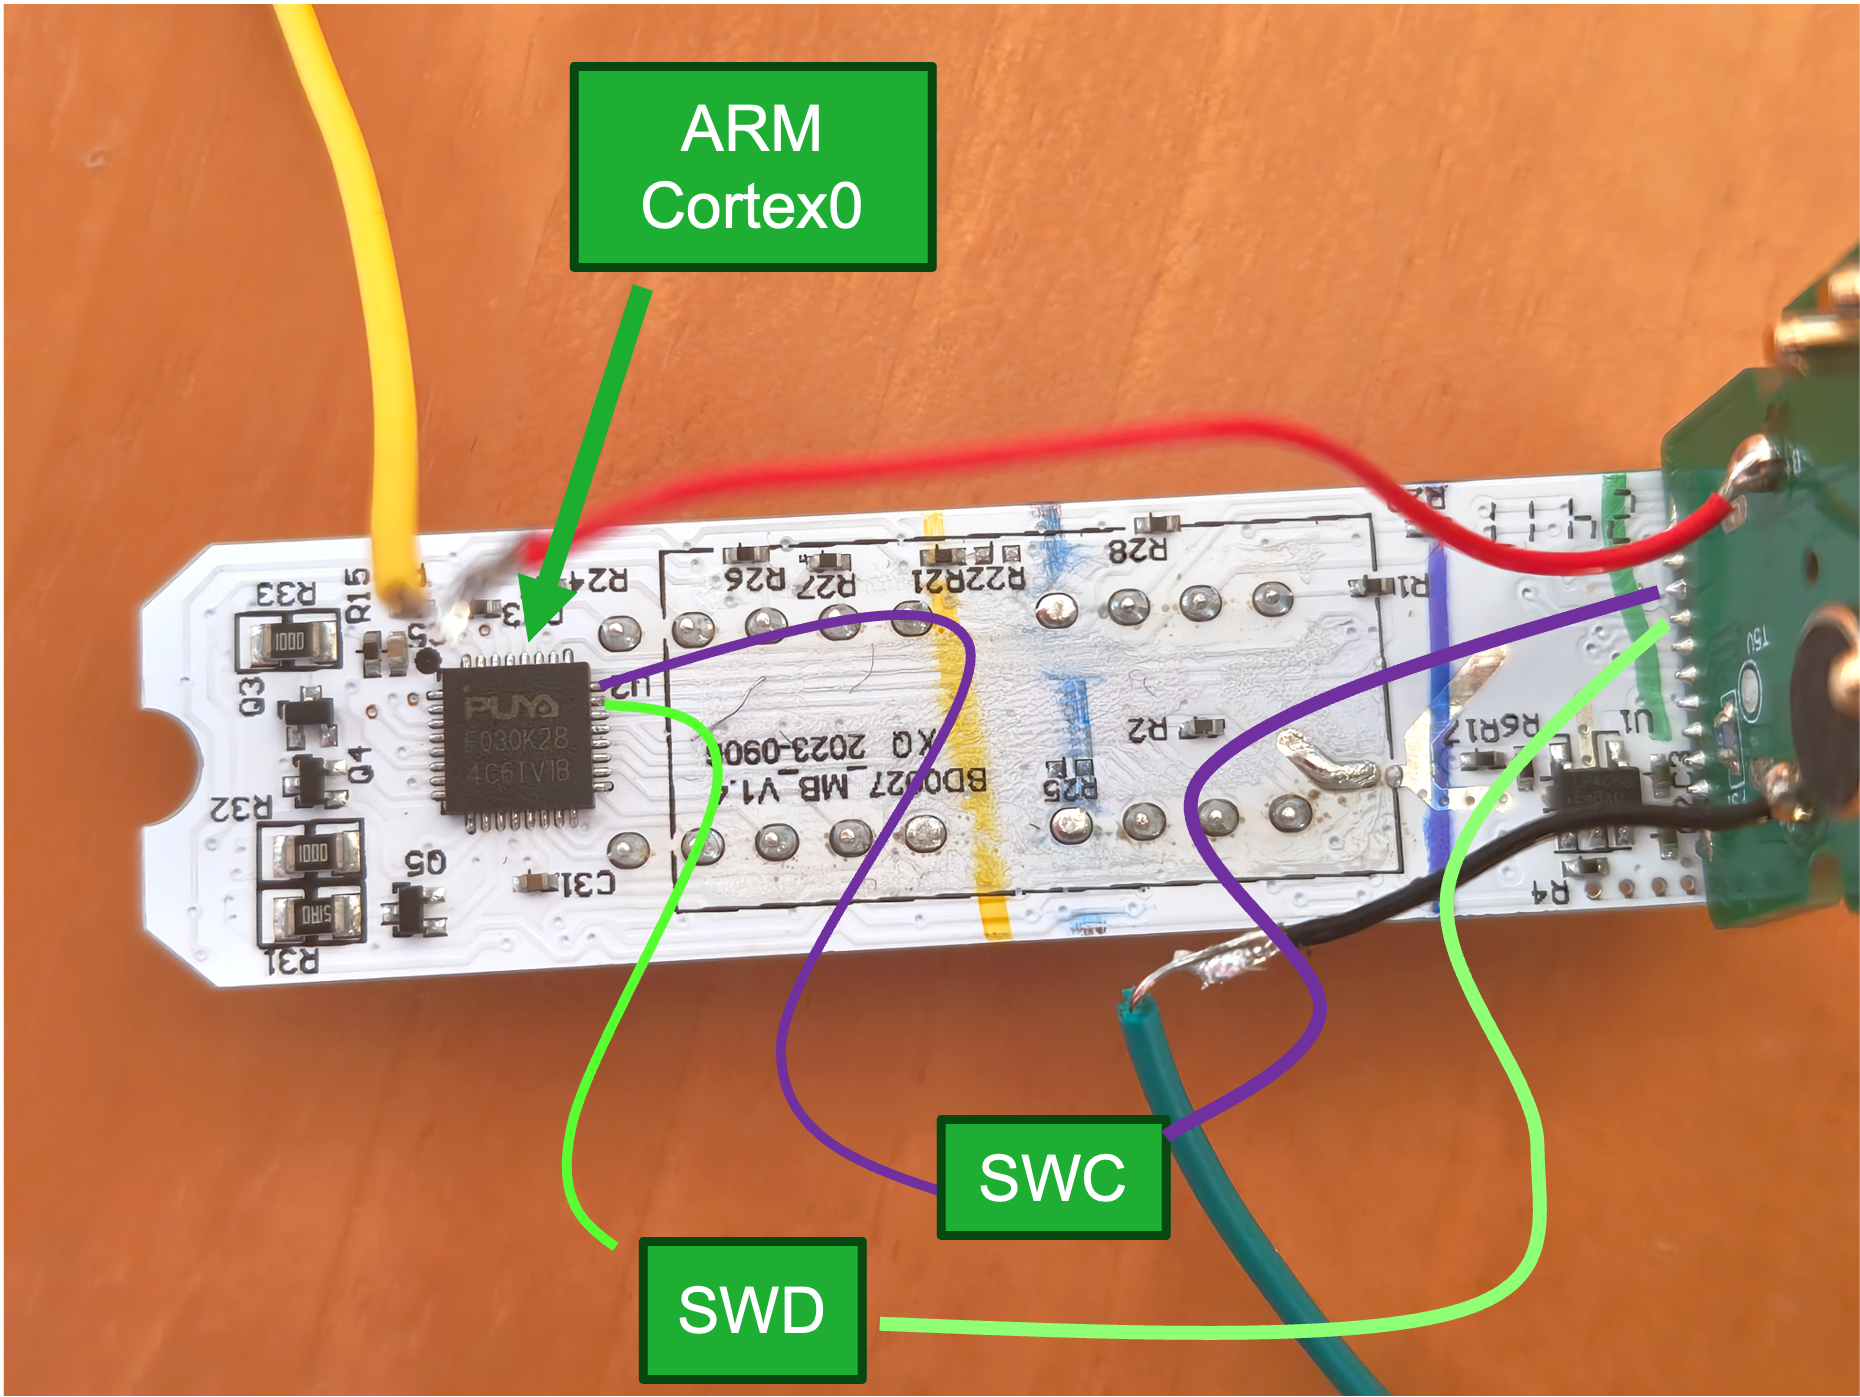
\includegraphics[width=.7\textwidth]{assets/board_2}
			\end{figure}
		\end{frame}
	\end{NoHyper}

   \begin{NoHyper}
        \begin{frame}{Setup details}
			\begin{figure}
				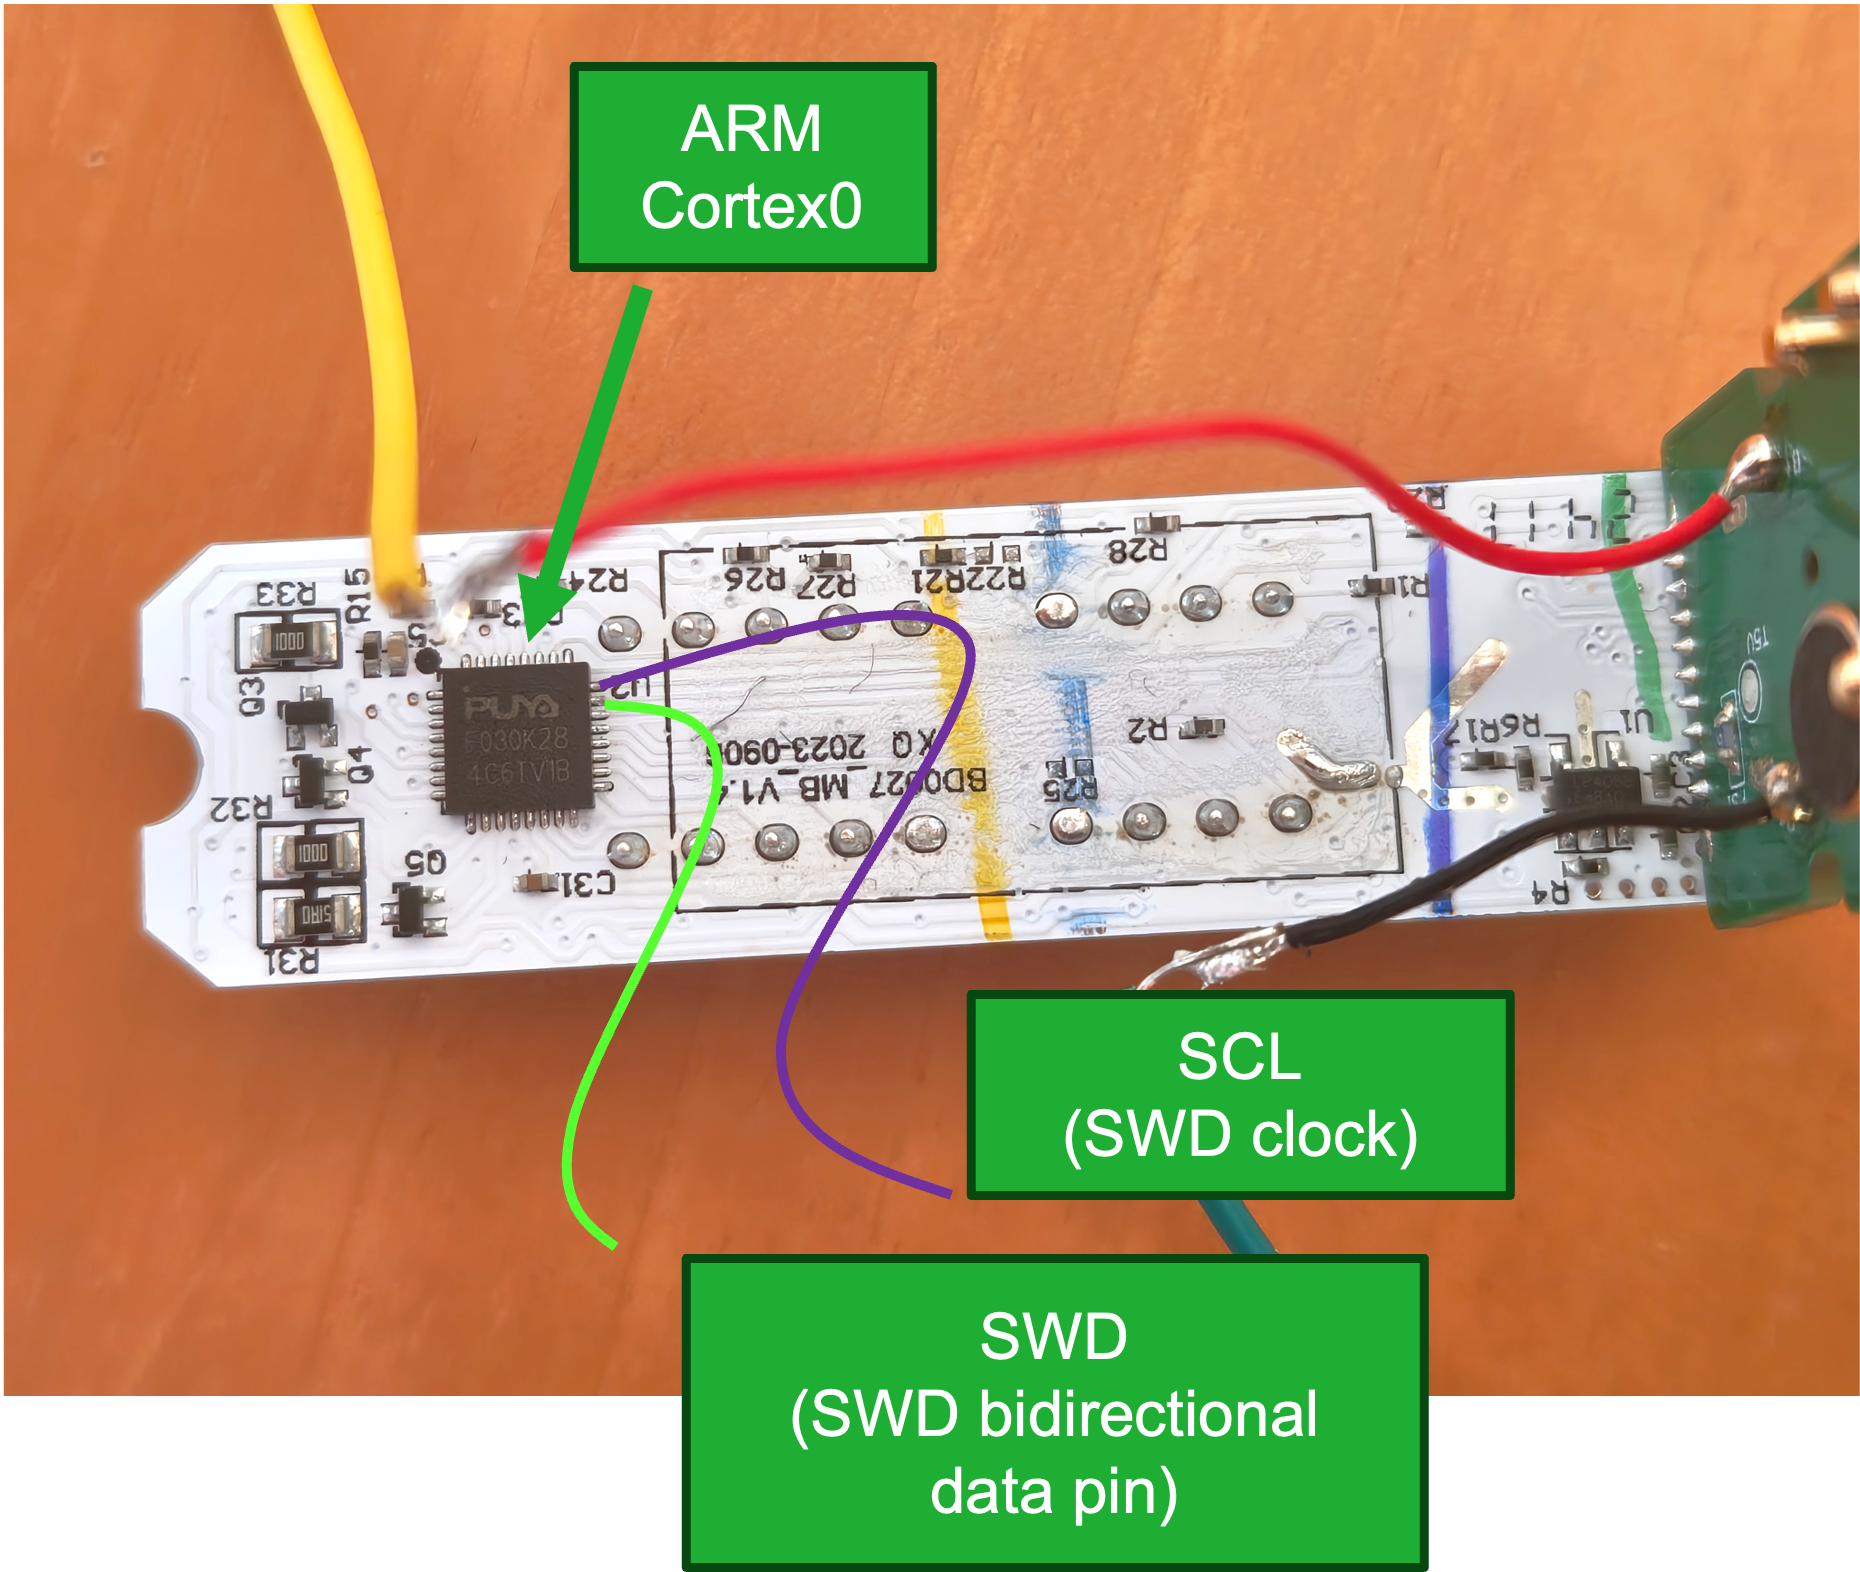
\includegraphics[width=.7\textwidth]{assets/board_3}
			\end{figure}
		\end{frame}
	\end{NoHyper}

   \begin{NoHyper}
        \begin{frame}{Setup details}
			\begin{figure}
				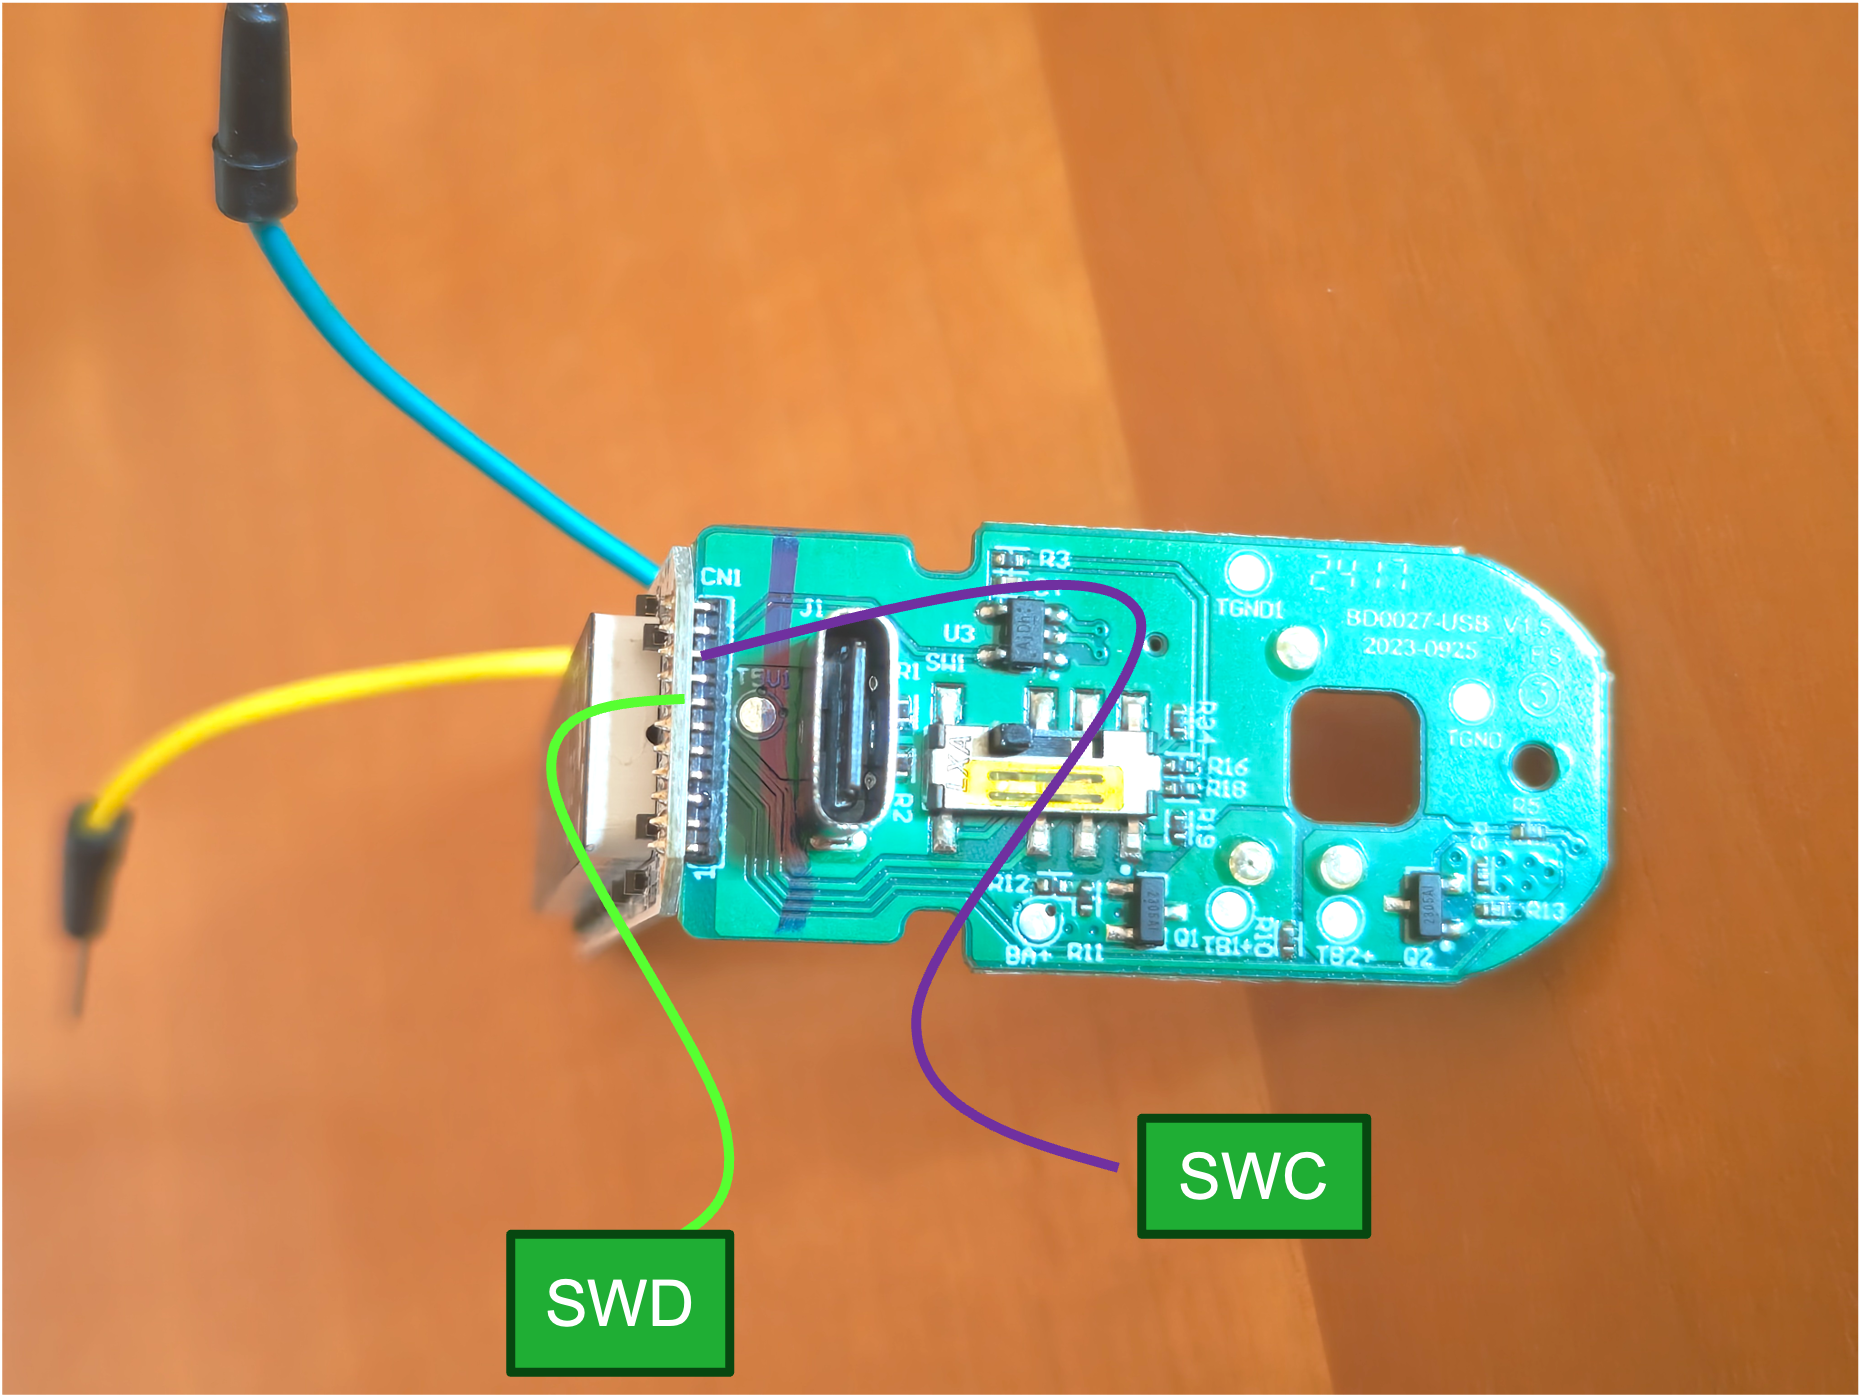
\includegraphics[width=.7\textwidth]{assets/board_4}
			\end{figure}
		\end{frame}
	\end{NoHyper}

   \begin{NoHyper}
        \begin{frame}{Usb-C soldering}
			By probing around more with the multimeter, we eventually discovered that we could reach SWD through USB-C
			\begin{figure}[t!]
				\subfloat{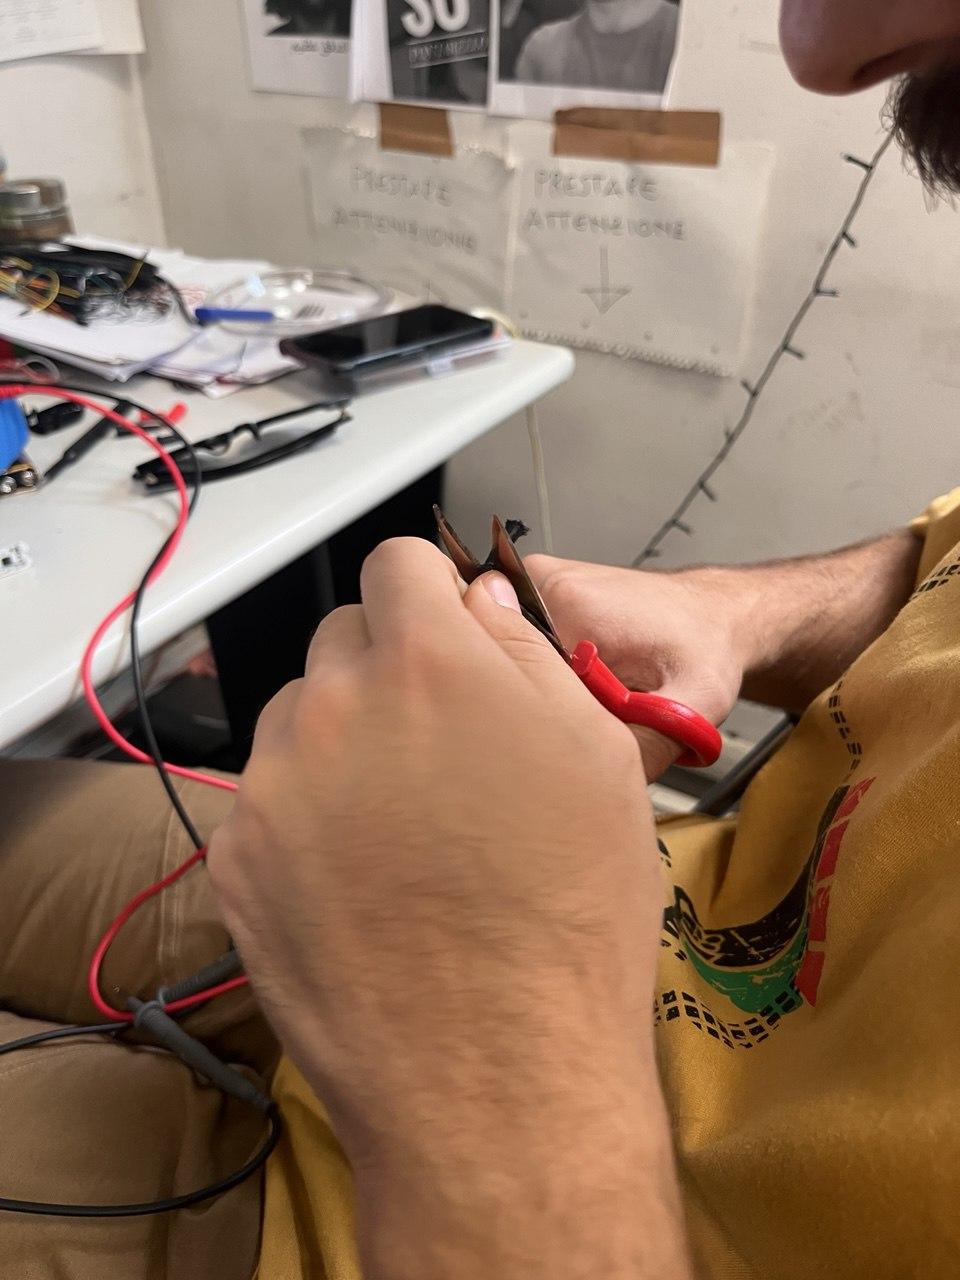
\includegraphics[width=0.3\linewidth]{assets/usbc_1.jpg}}\hfill
				\subfloat{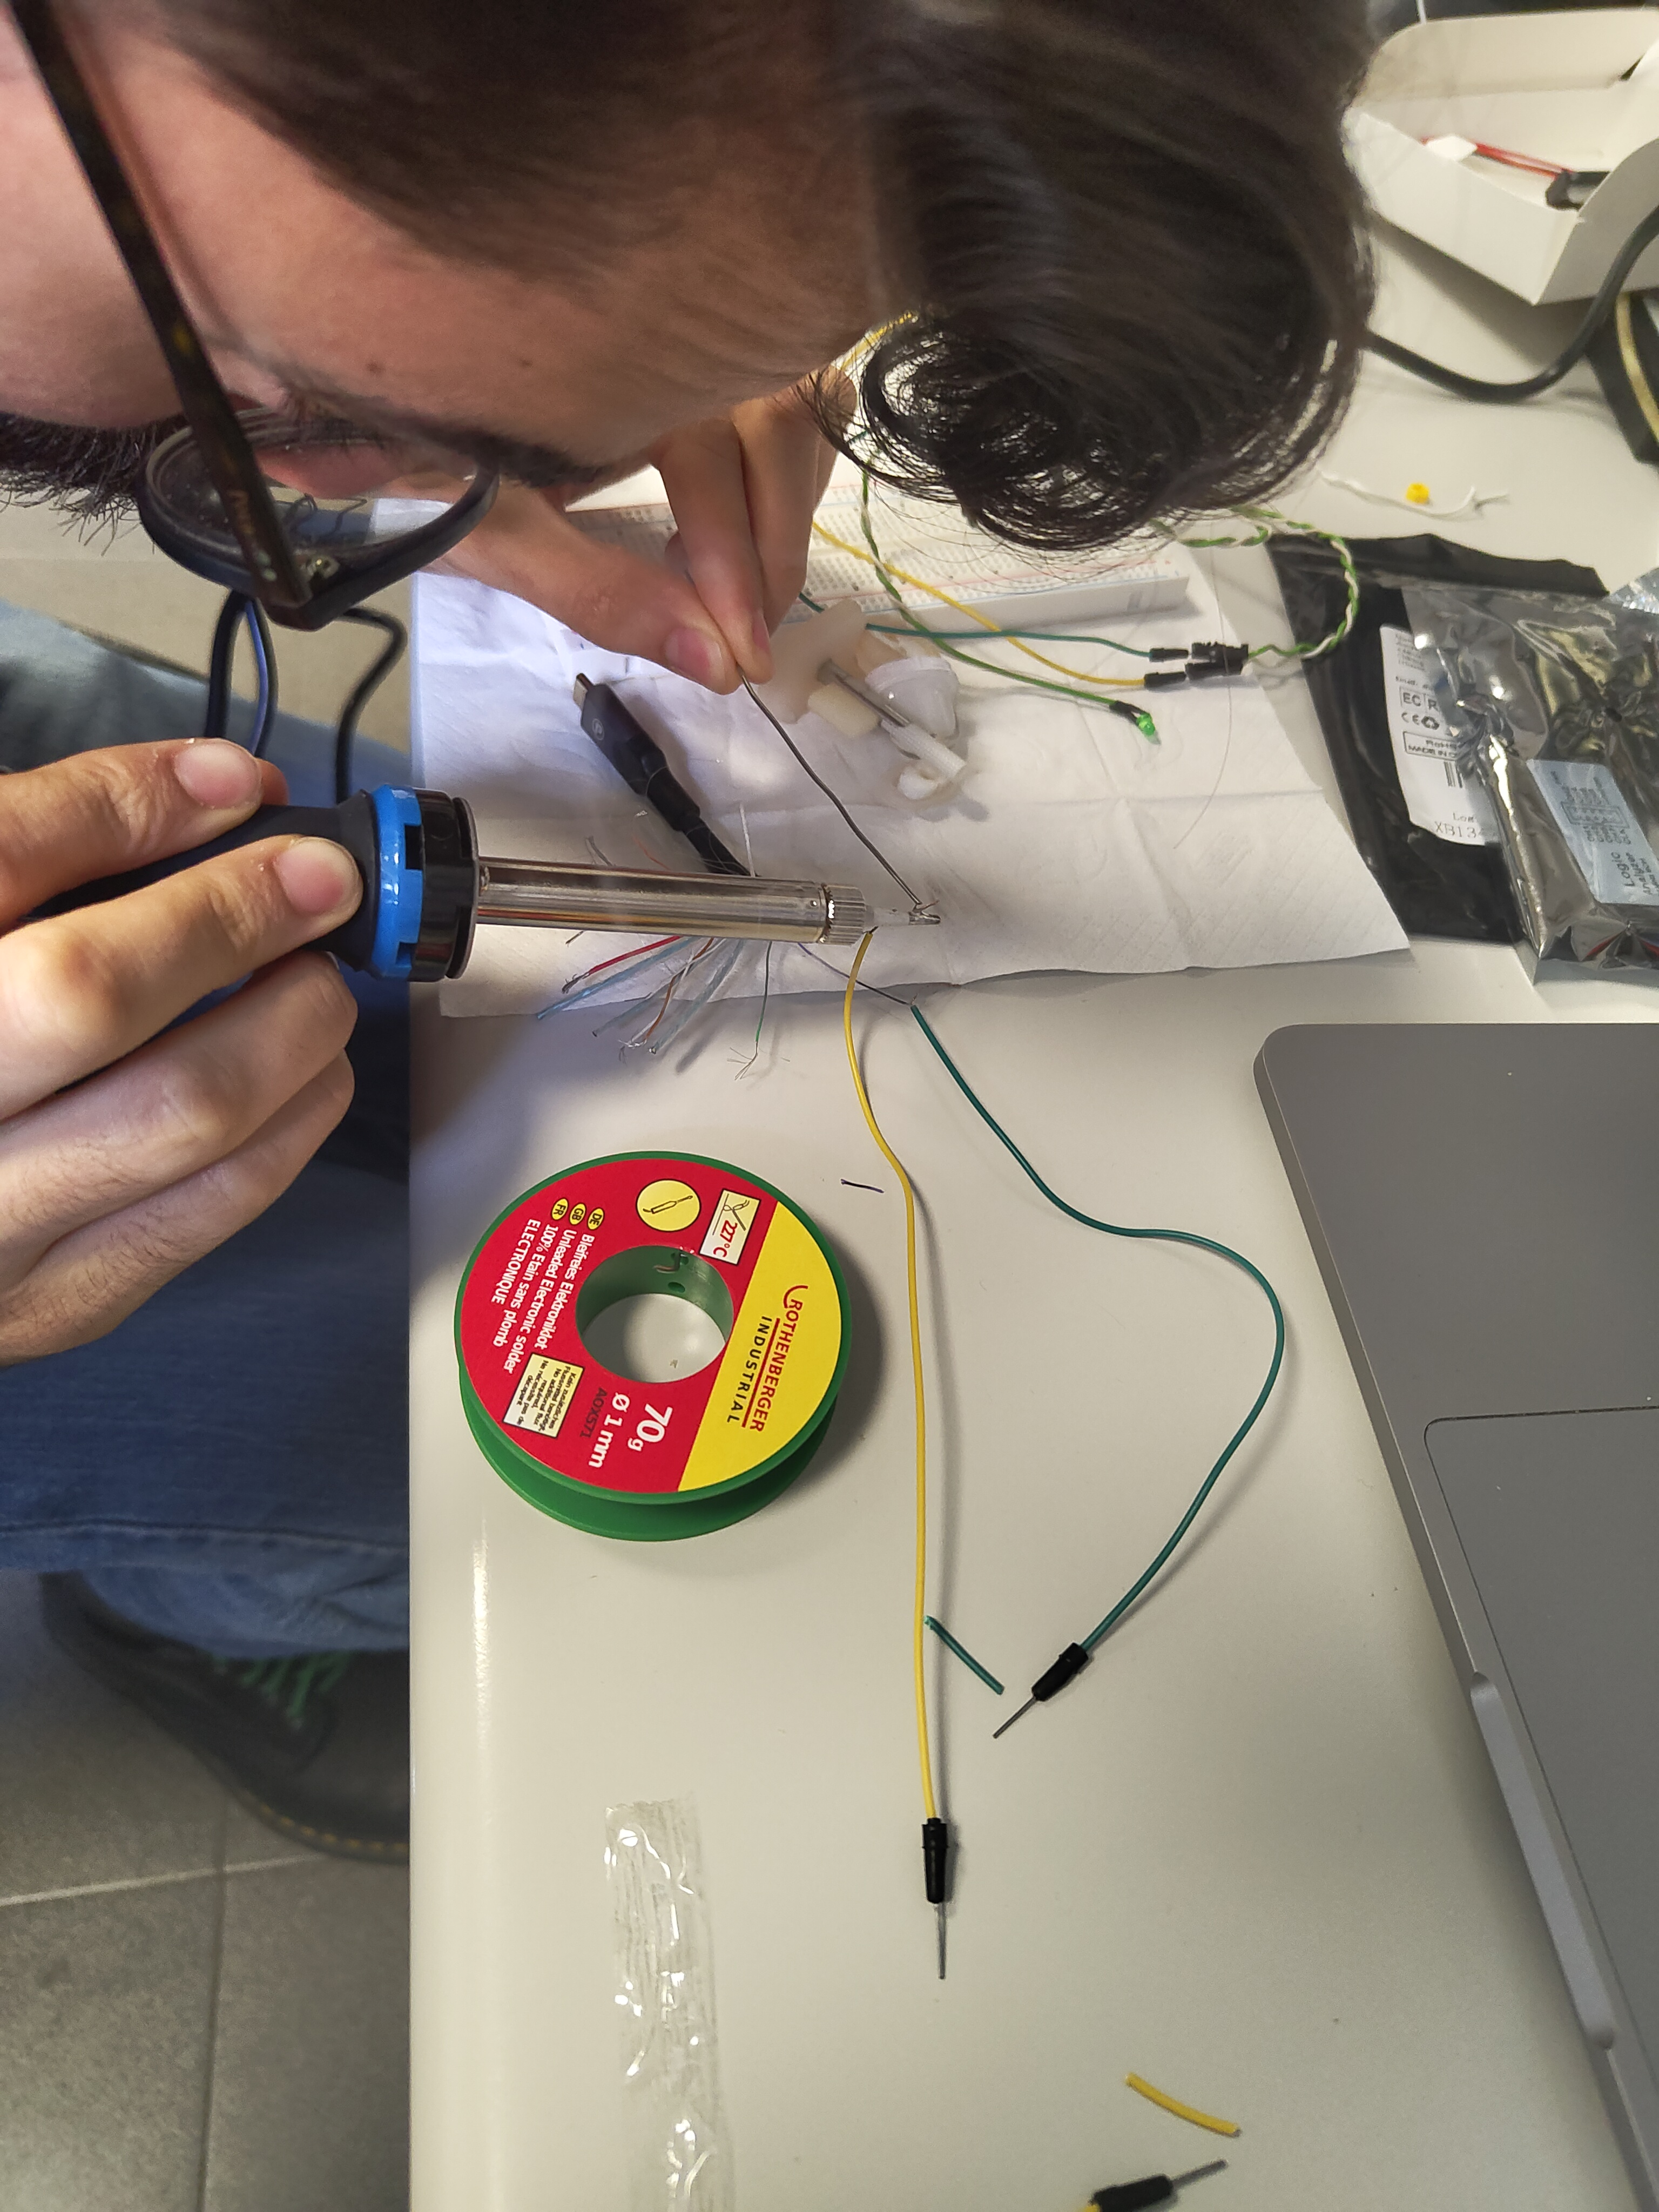
\includegraphics[width=0.3\linewidth]{assets/solder_usbc.jpg}}\hfill
  				\subfloat{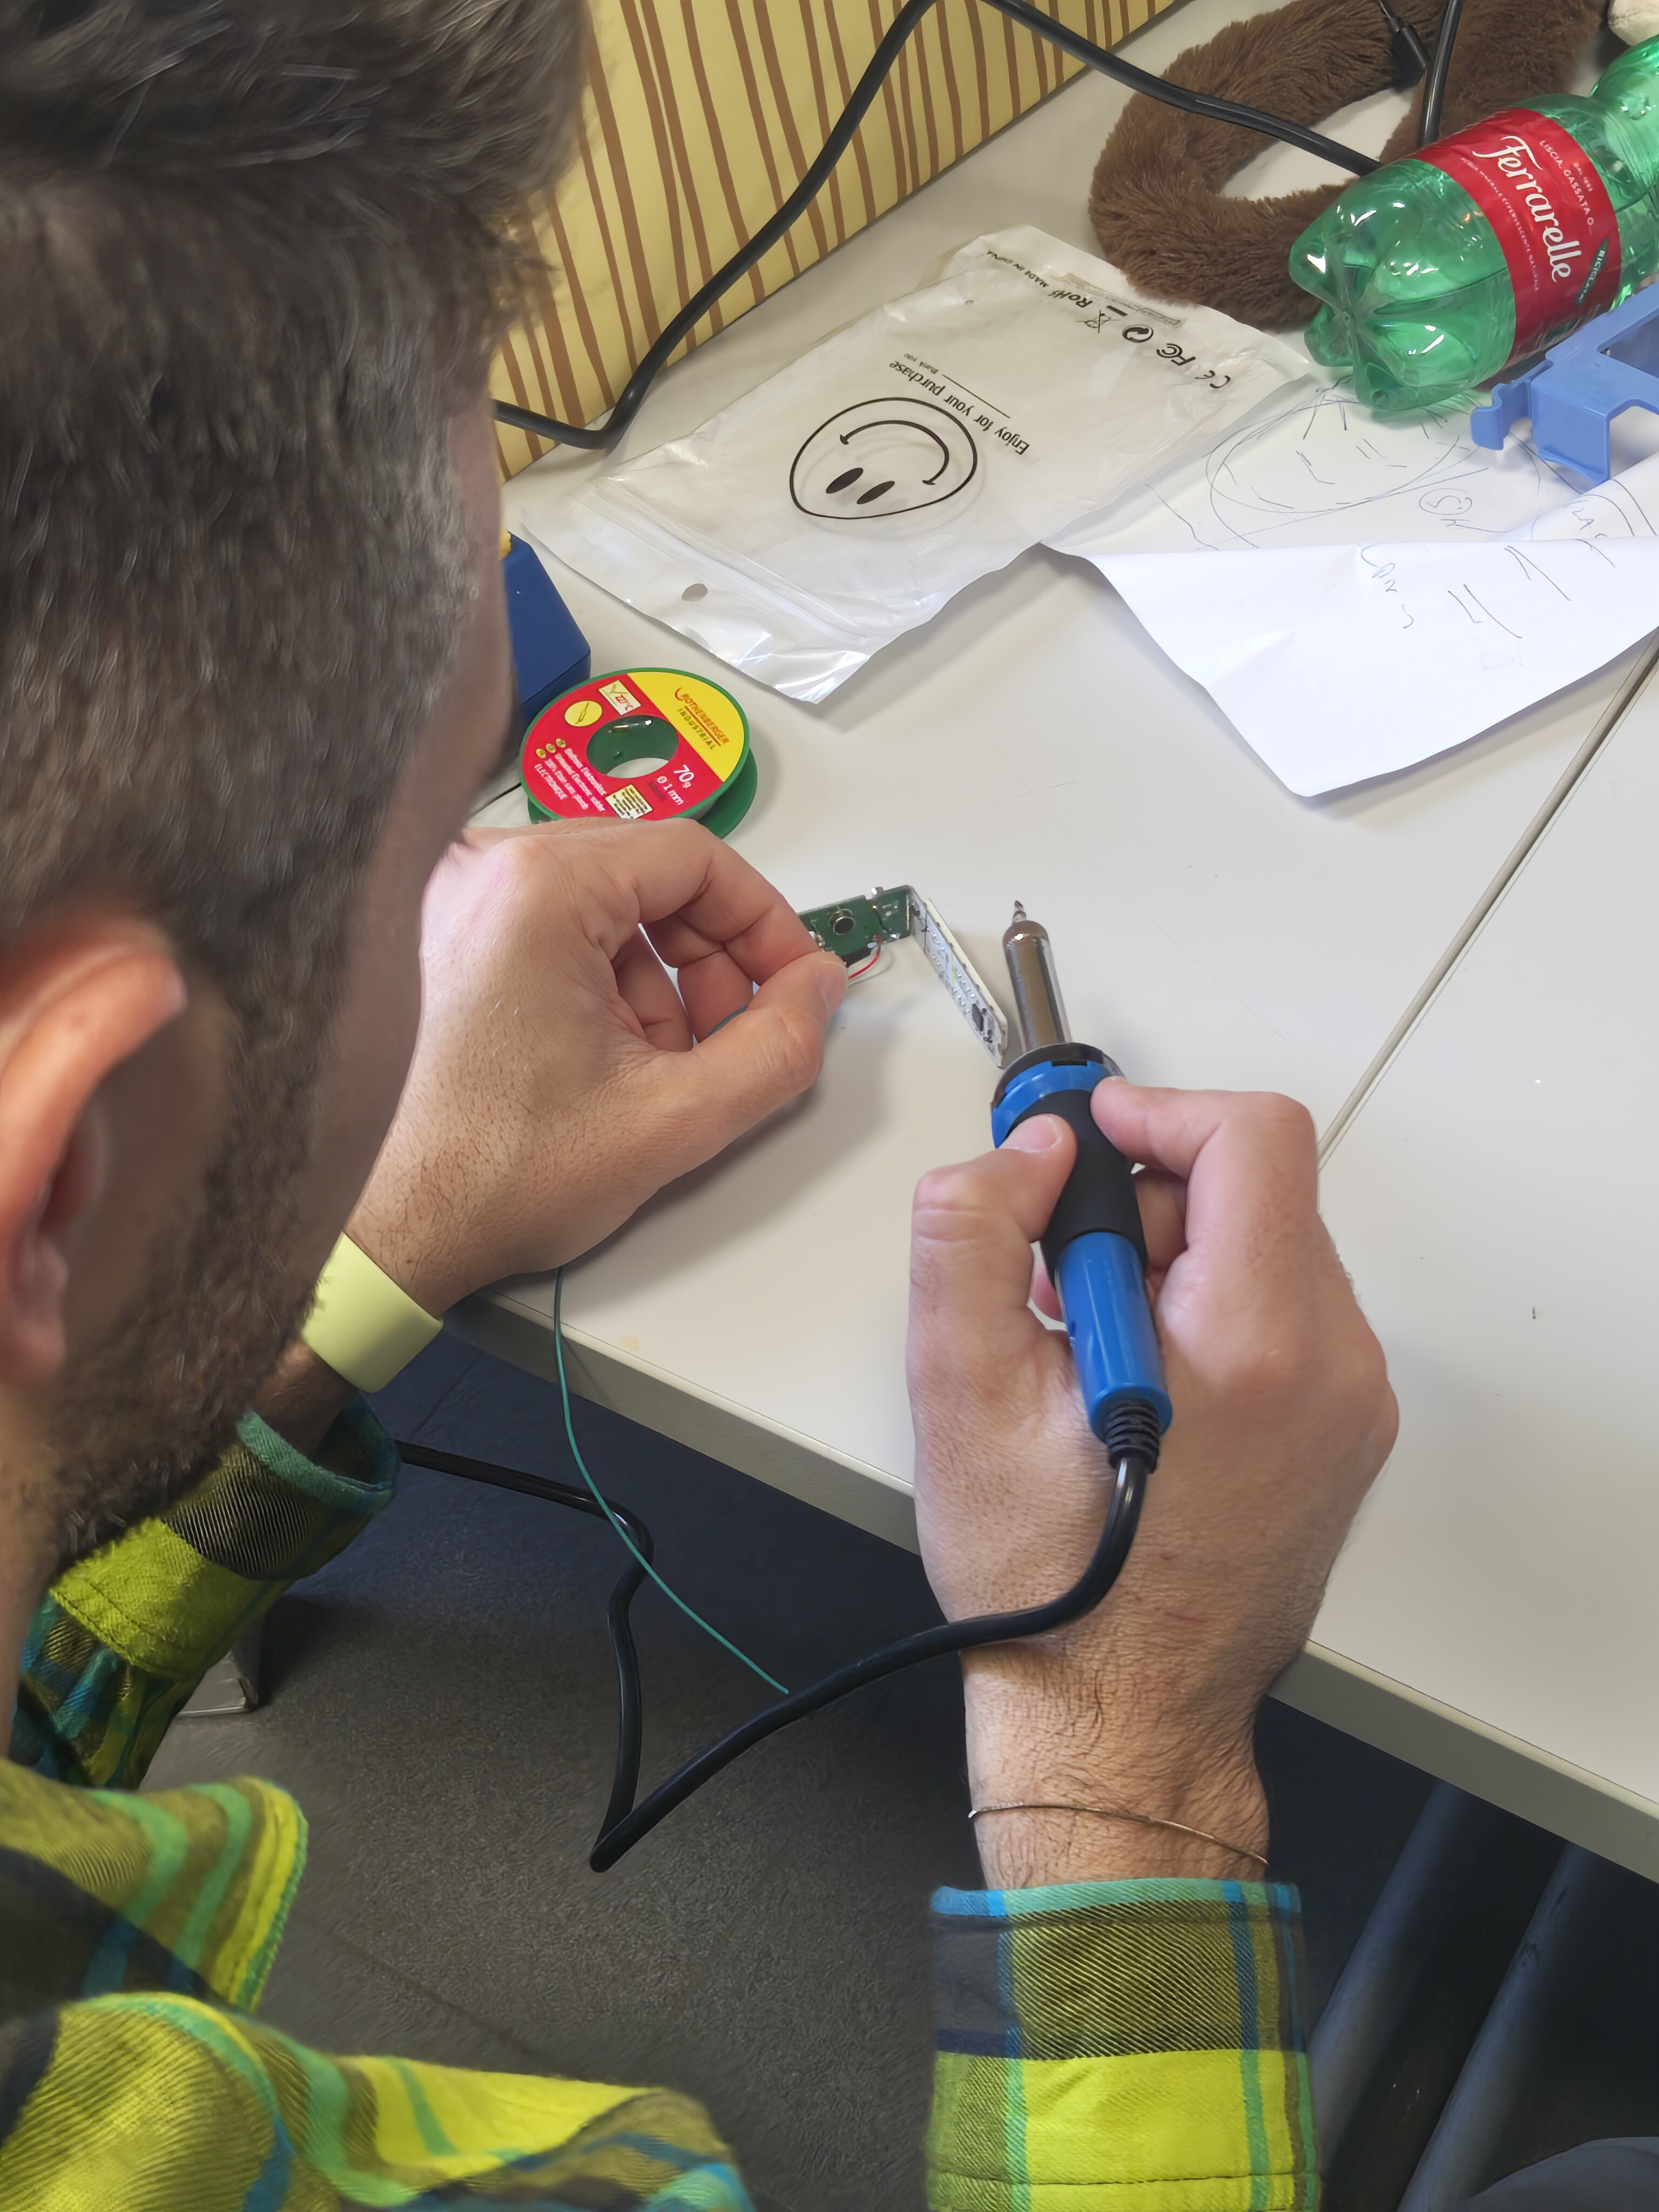
\includegraphics[width=0.3\linewidth]{assets/lucaa_1.jpg}}\hfill%
			\end{figure}
		\end{frame}
	\end{NoHyper}

   \begin{NoHyper}
        \begin{frame}{Our final setup}
			\begin{figure}
				\centering
				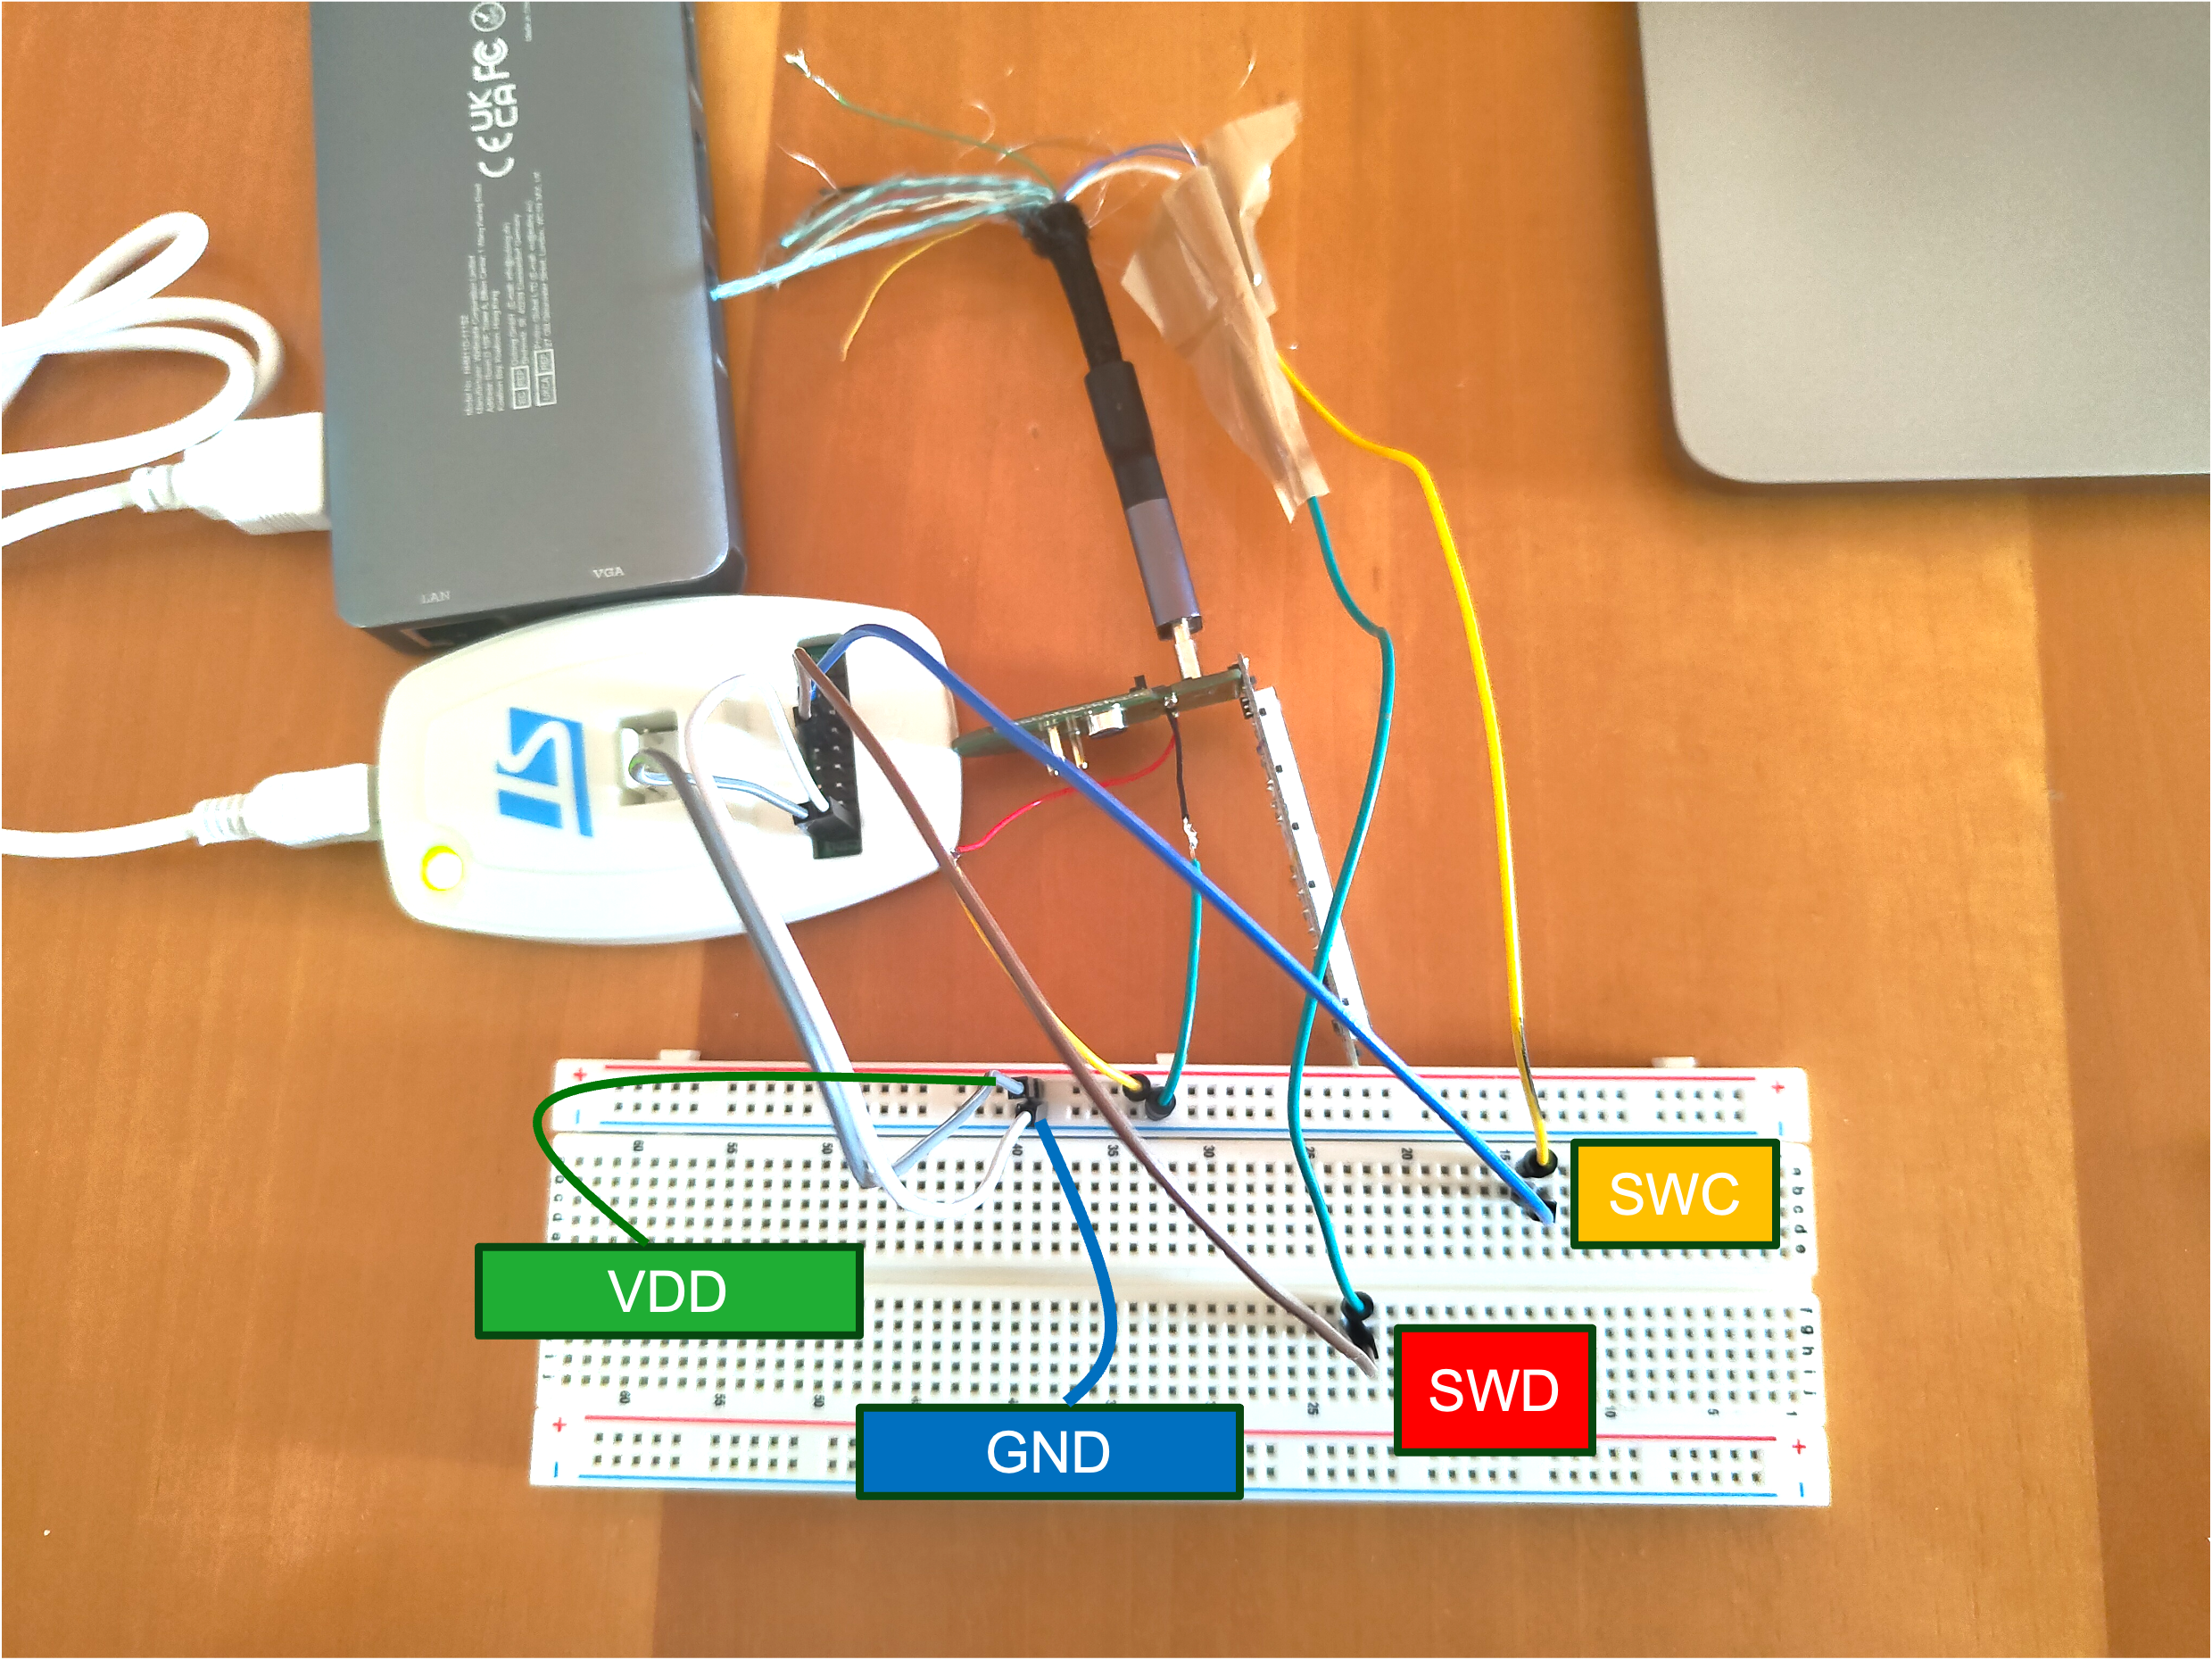
\includegraphics[width=.7\textwidth]{assets/final_setup}
			\end{figure}
		\end{frame}
	\end{NoHyper}

   \begin{NoHyper}
        \begin{frame}{JLink connection}
			\texttt{pyocd} could detect the STJLink device, but connectiing through SWD would fail over and over
			\begin{figure}[t!]
				\subfloat{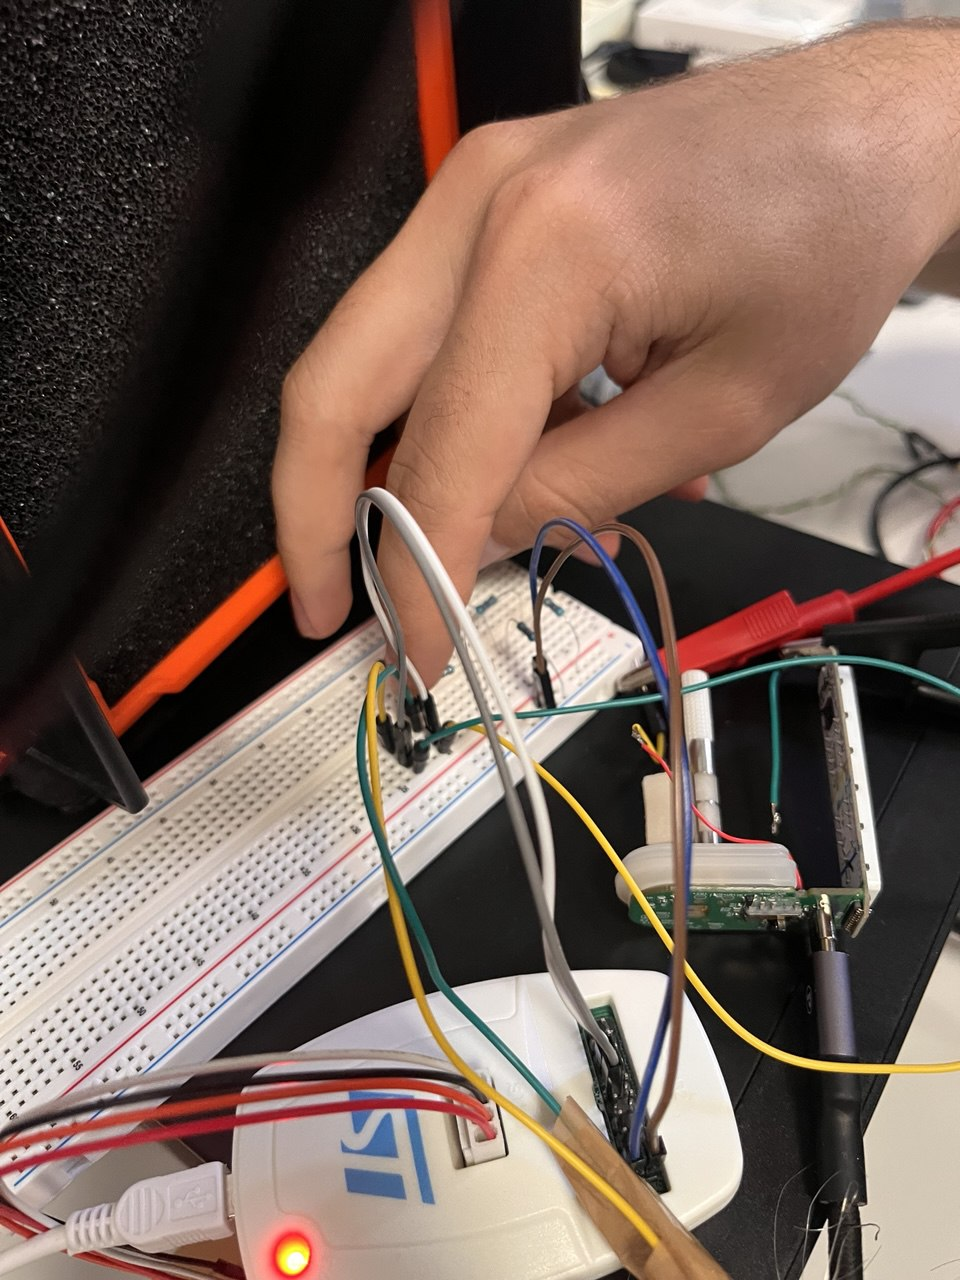
\includegraphics[width=0.3\linewidth]{assets/jlink_1.jpg}}\hfill
				\subfloat{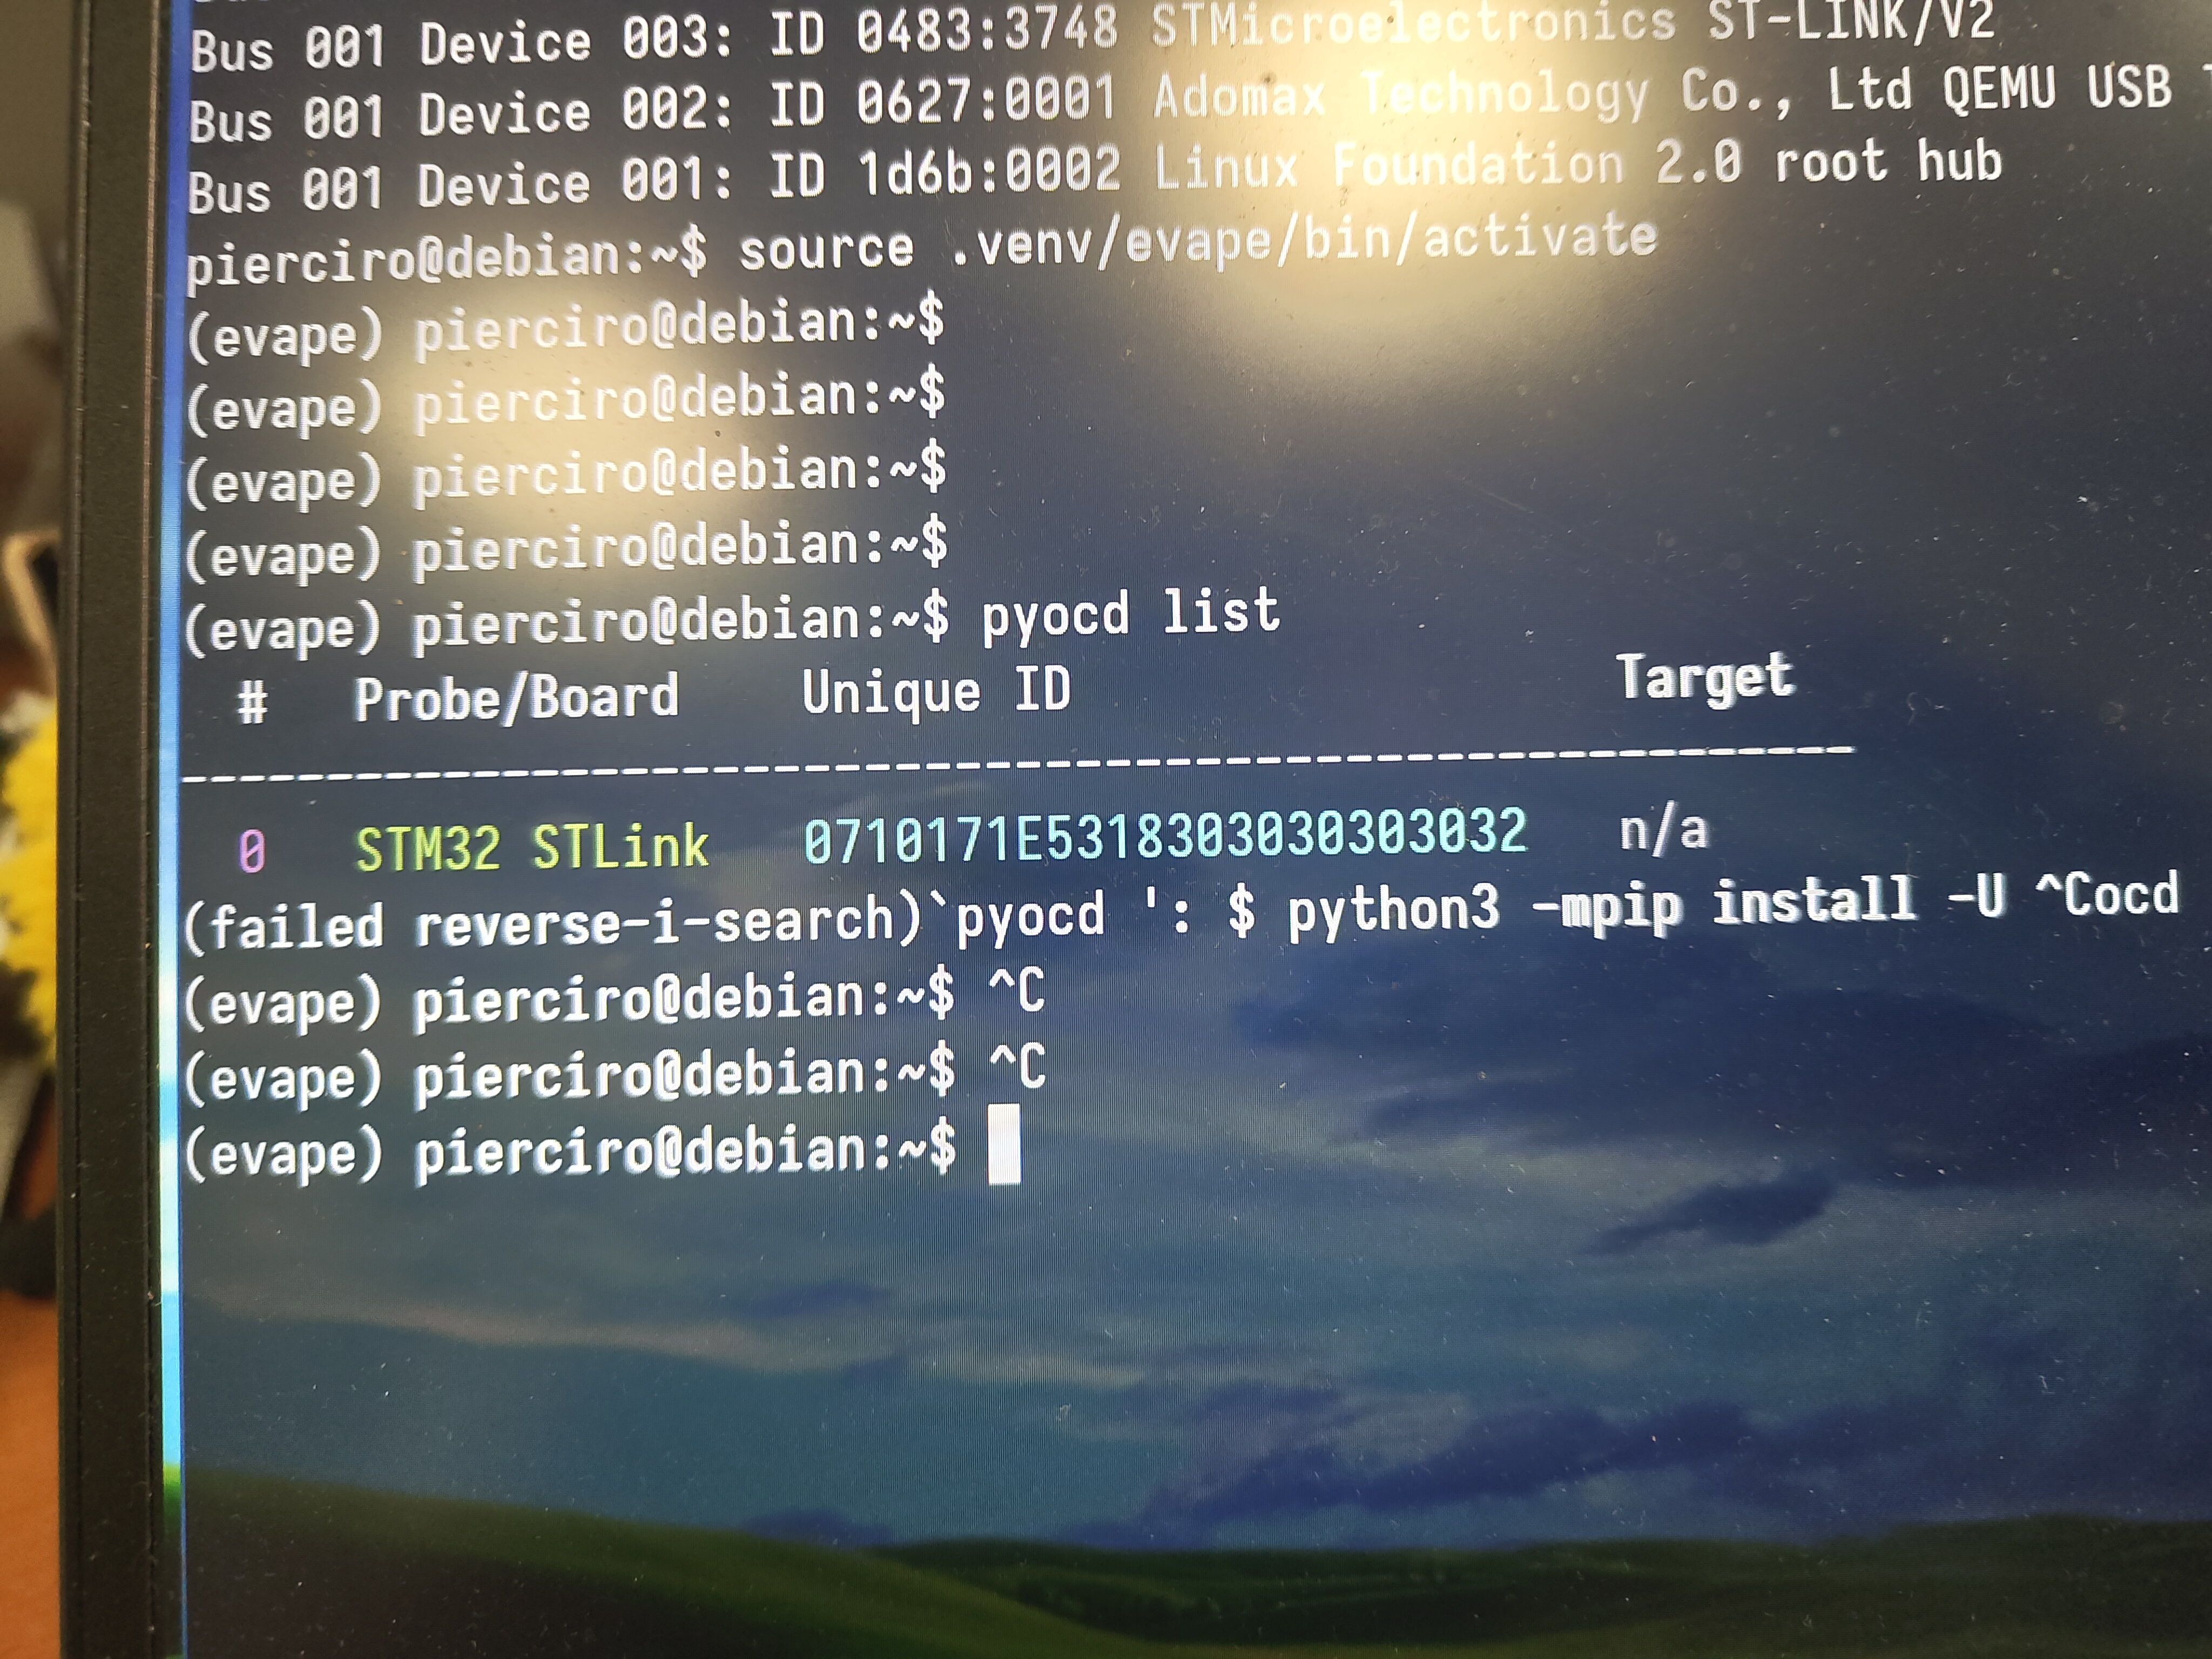
\includegraphics[width=0.3\linewidth]{assets/jlink_pyocd.jpg}}\hfill
  				\subfloat{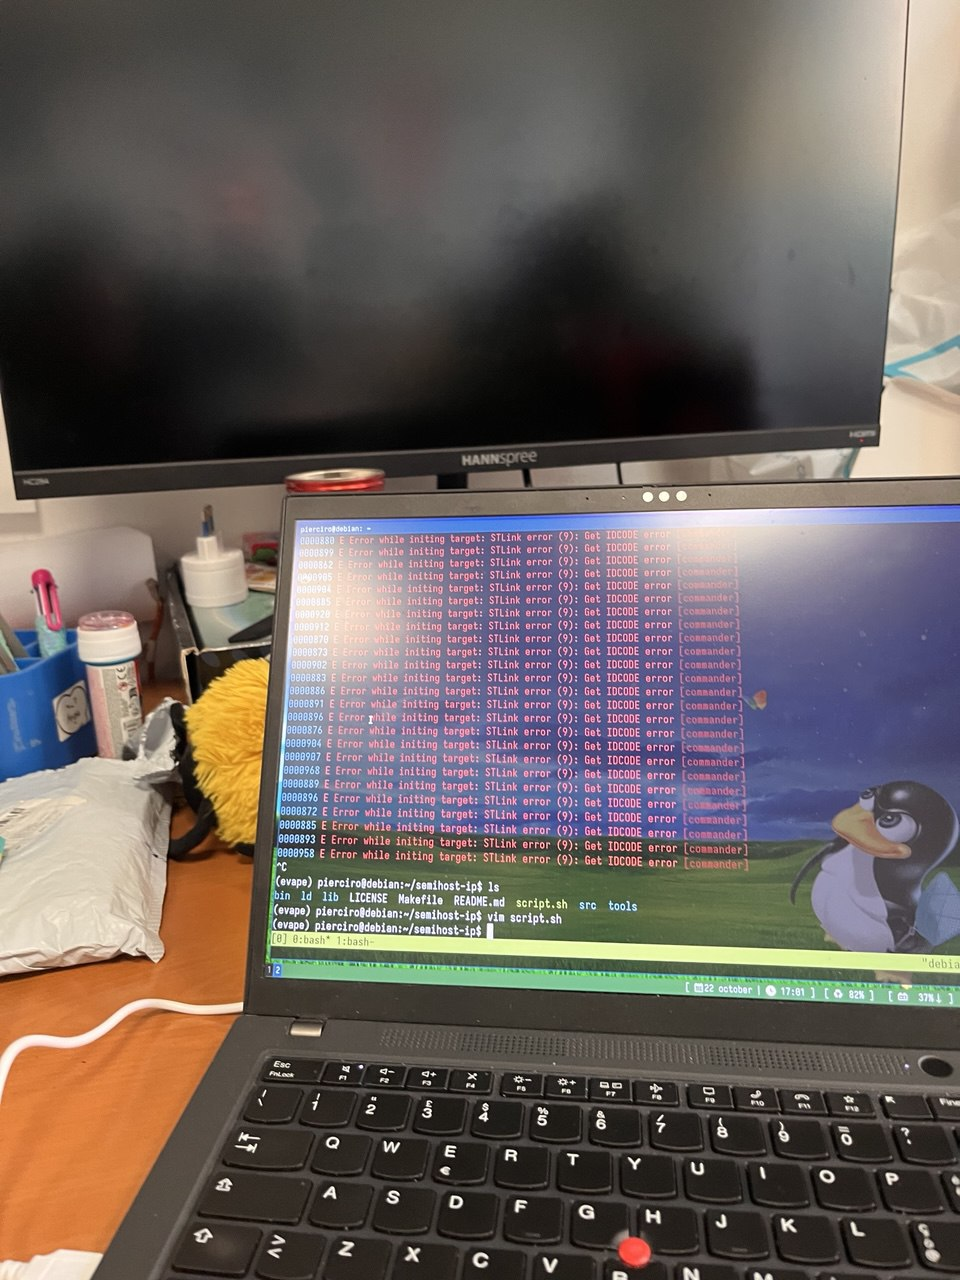
\includegraphics[width=0.3\linewidth]{assets/jlink_error.jpg}}\hfill%
			\end{figure}
		\end{frame}
	\end{NoHyper}

   \begin{NoHyper}
        \begin{frame}{JLink connection}
			\begin{itemize}
				\item At this point, we tried several paths
				\item We reached Bogdan (the original author of the blogpost), who suggested us to power up the vape from the JLink and to check if we would need to swap SWD and CLK
				\item We started to think that we needed our eVape always ON, so we needed a way to do this
				\item Problems, problems, problems ...
			\end{itemize}
		\end{frame}
	\end{NoHyper}

   \begin{NoHyper}
        \begin{frame}{JLink signal with logic analyzer}
			We used a logic analyzer to display SWD signal and check weather the connection was actually taking place or not
			\begin{figure}
				\centering
				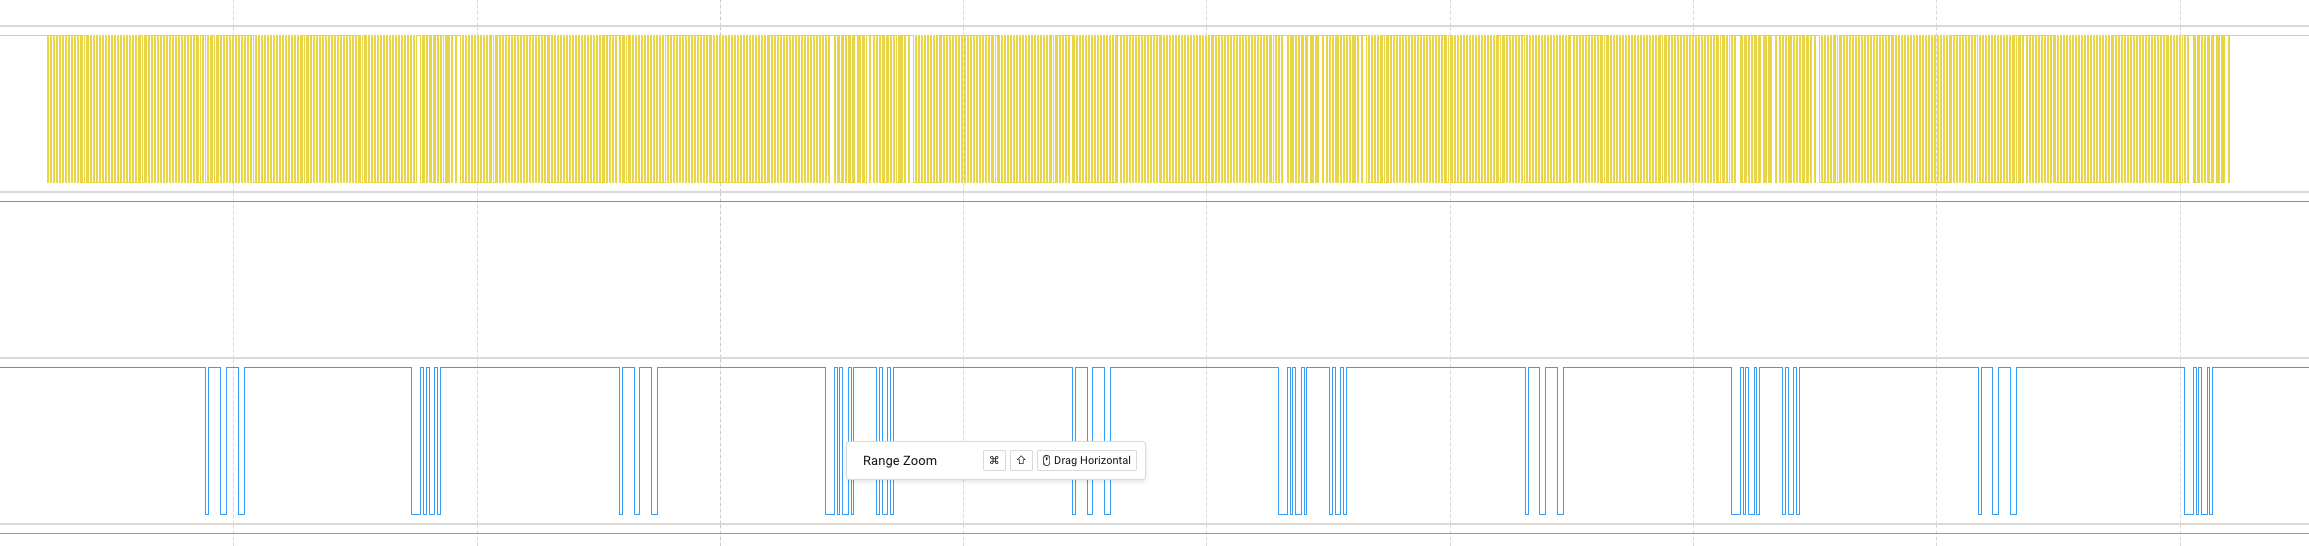
\includegraphics[width=\textwidth]{assets/oscilloscope}
			\end{figure}
		\end{frame}
	\end{NoHyper}

   \begin{NoHyper}
        \begin{frame}{Bogdan helping us once again!}
			\begin{figure}
				\centering
				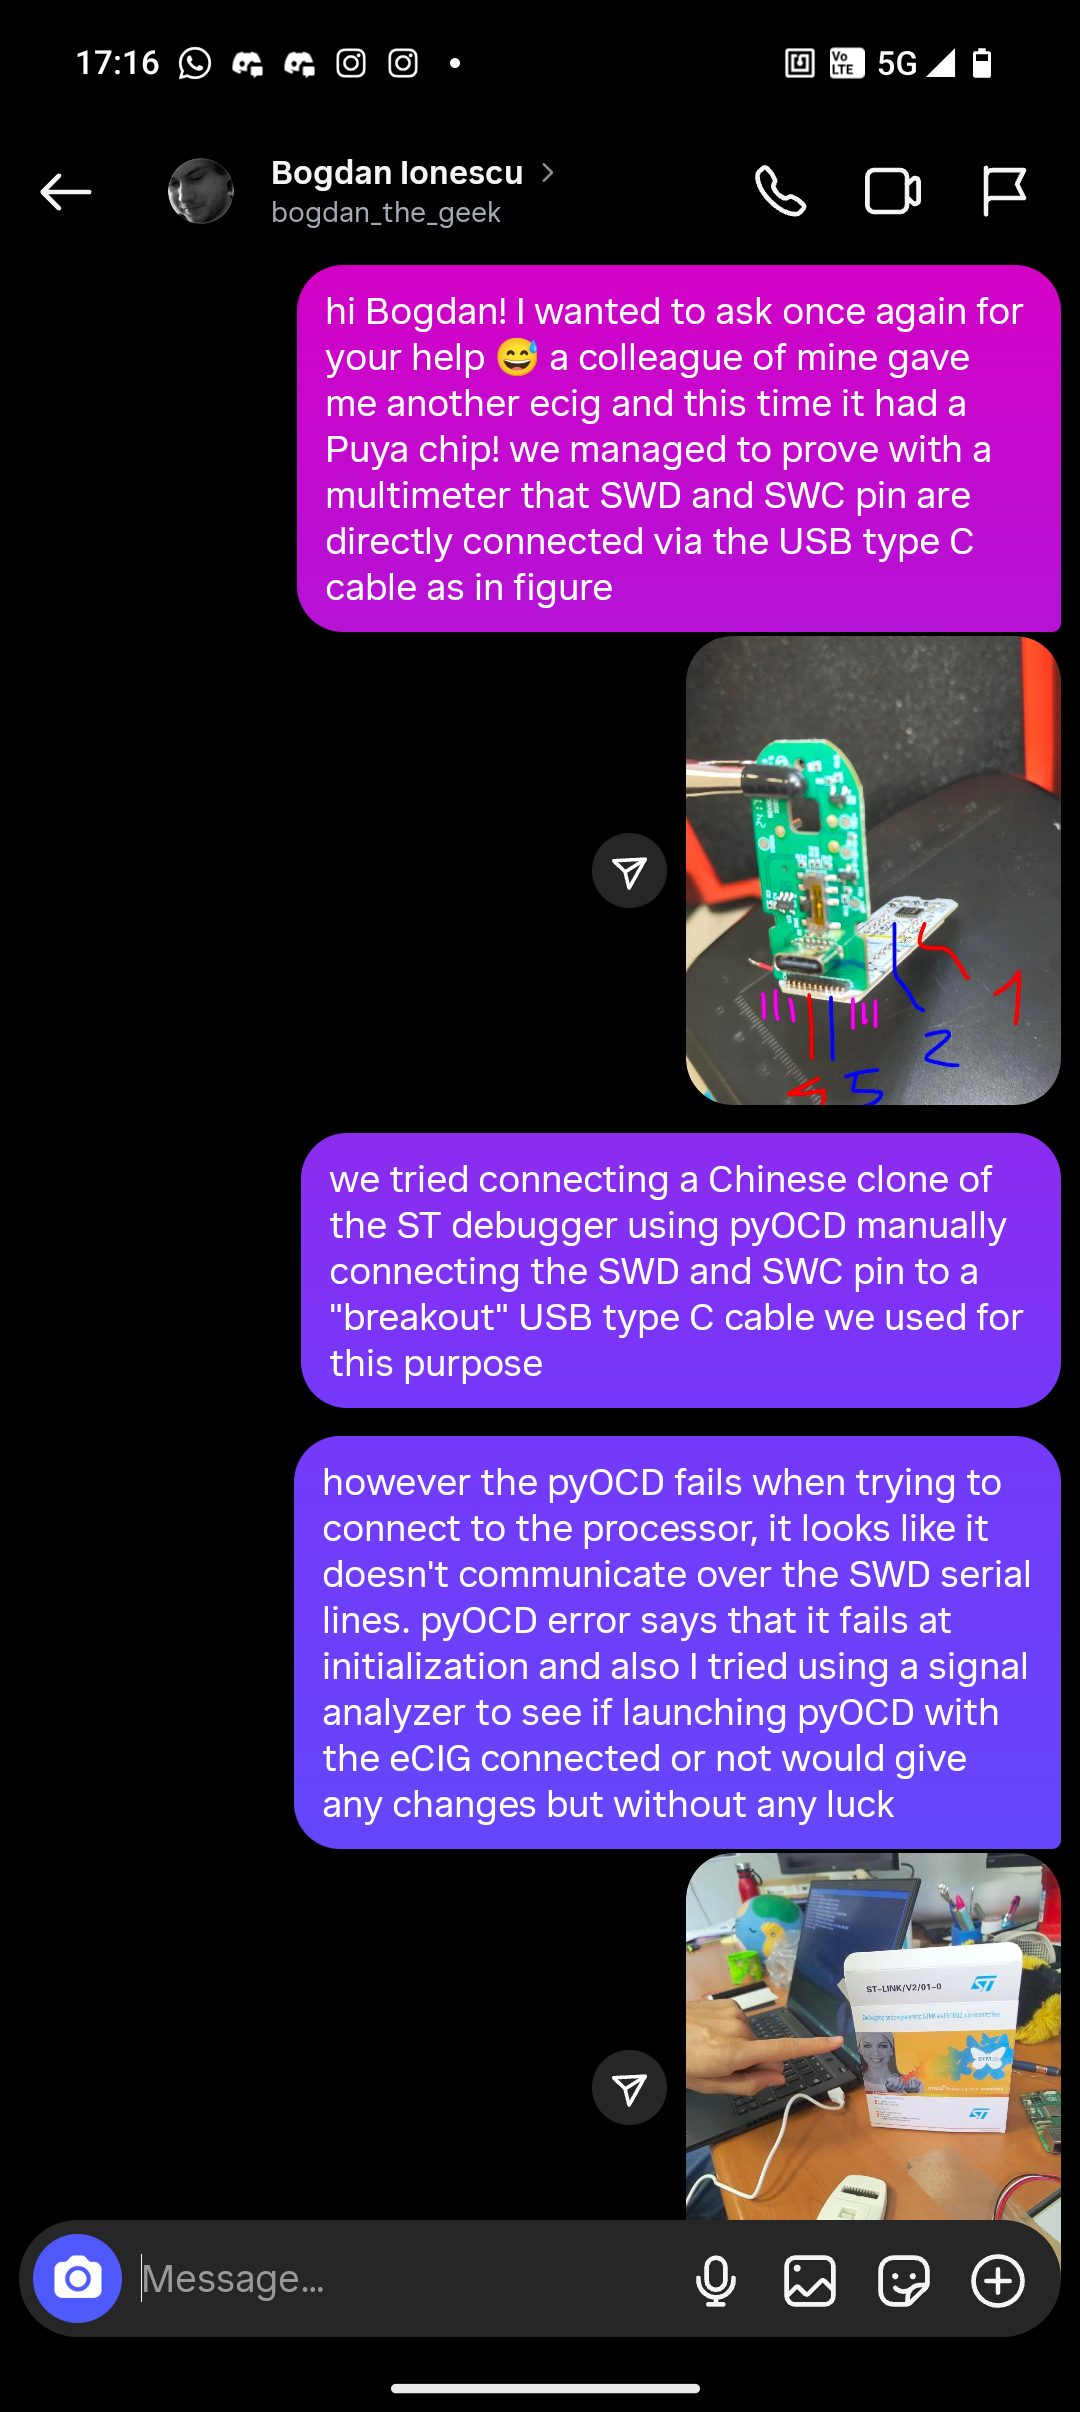
\includegraphics[width=.3\textwidth]{assets/bogdan_4}
			\end{figure}
			%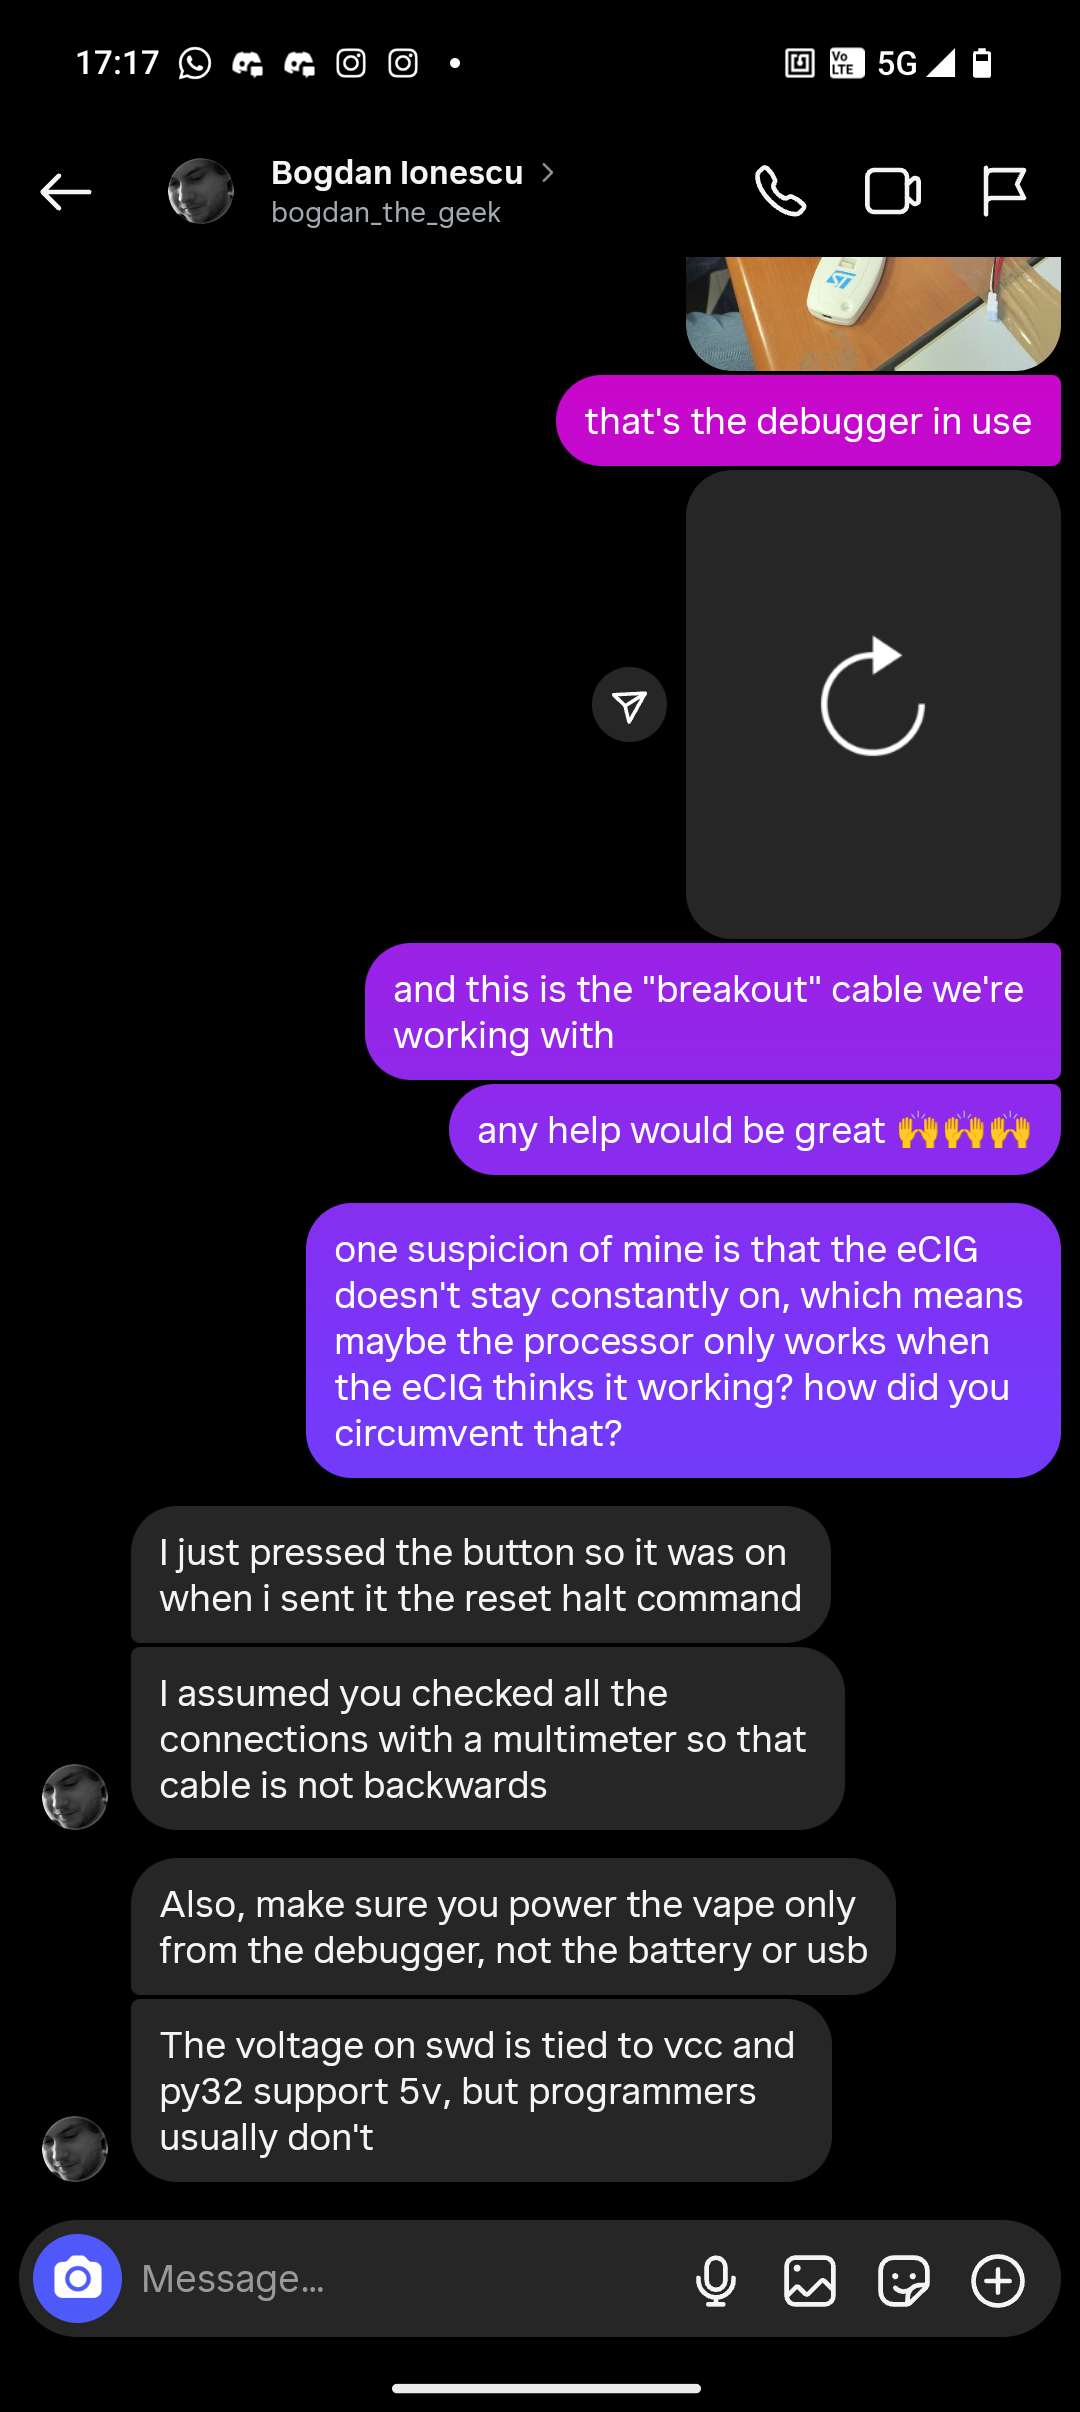
\includegraphics[width=.7\textwidth]{assets/bogdan_5}
		\end{frame}
	\end{NoHyper}

   \begin{NoHyper}
        \begin{frame}{Bogdan helping us once again!}
			\begin{figure}
				\centering
				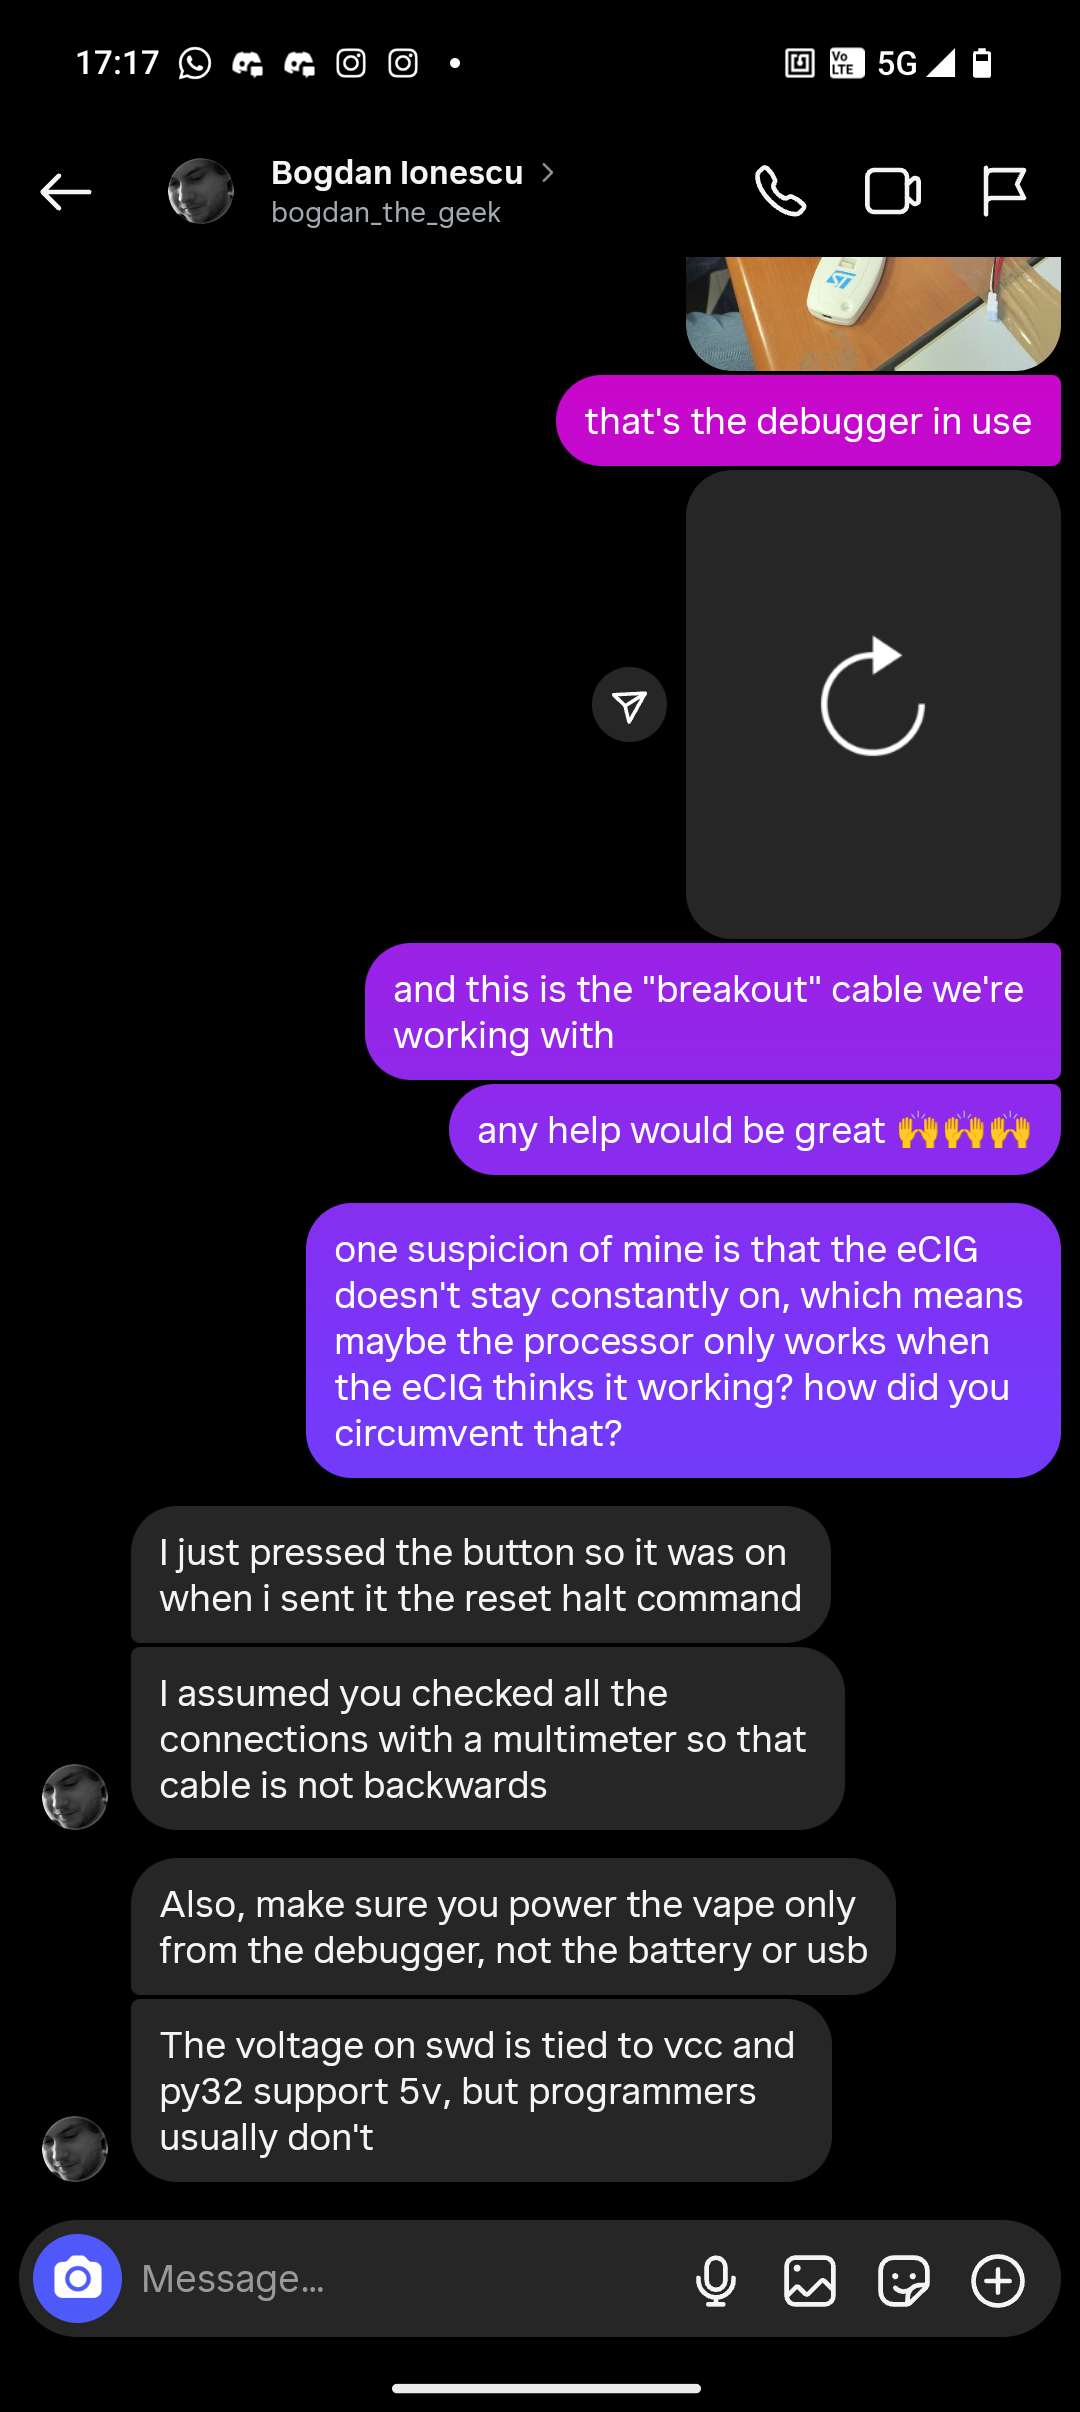
\includegraphics[width=.3\textwidth]{assets/bogdan_5}
			\end{figure}
			%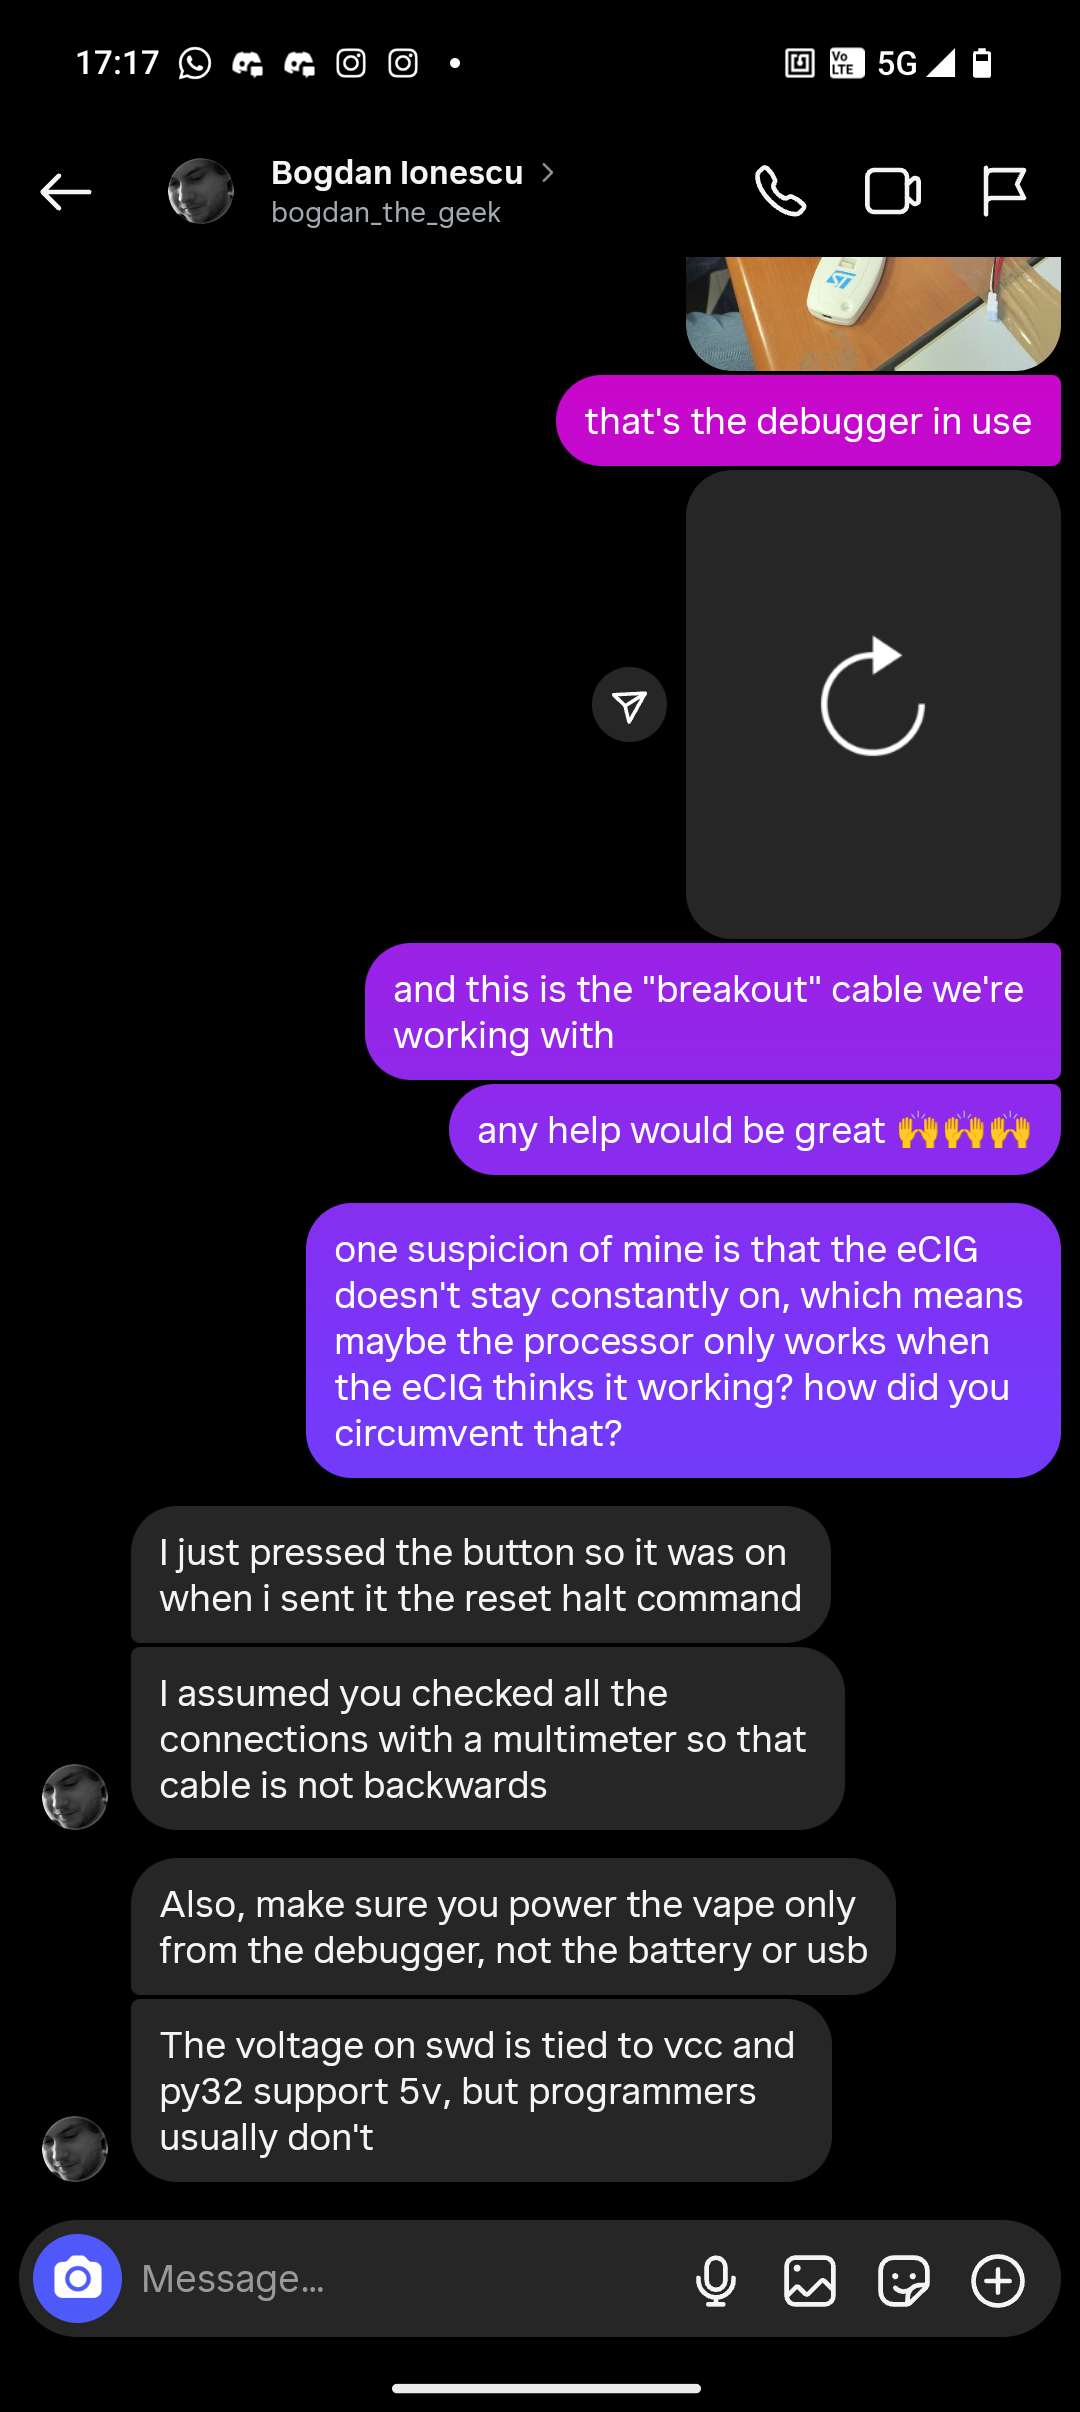
\includegraphics[width=.7\textwidth]{assets/bogdan_5}
		\end{frame}
	\end{NoHyper}

   \begin{NoHyper}
			\section{Atto IV}
			\frame{\sectionpage}
	\end{NoHyper}

   \begin{NoHyper}
        \begin{frame}{Lucaa, our saviour!}
			\begin{itemize}
				\item Luca had the idea that what was telling to the eVape to stay up was a pressure sensor
				\item We used Google lens to check out which sensor would actually mathc the right one
				\item \textbf{Engineering idea from Luca}: let's attach a plastic straw to the sensor and blow to keep it up
			\end{itemize}
		\end{frame}
	\end{NoHyper}

   \begin{NoHyper}
        \begin{frame}{EuLuka!}
			We managed to dump the eVape firmware using \texttt{pyocd}!
			\begin{figure}[t!]
				\subfloat{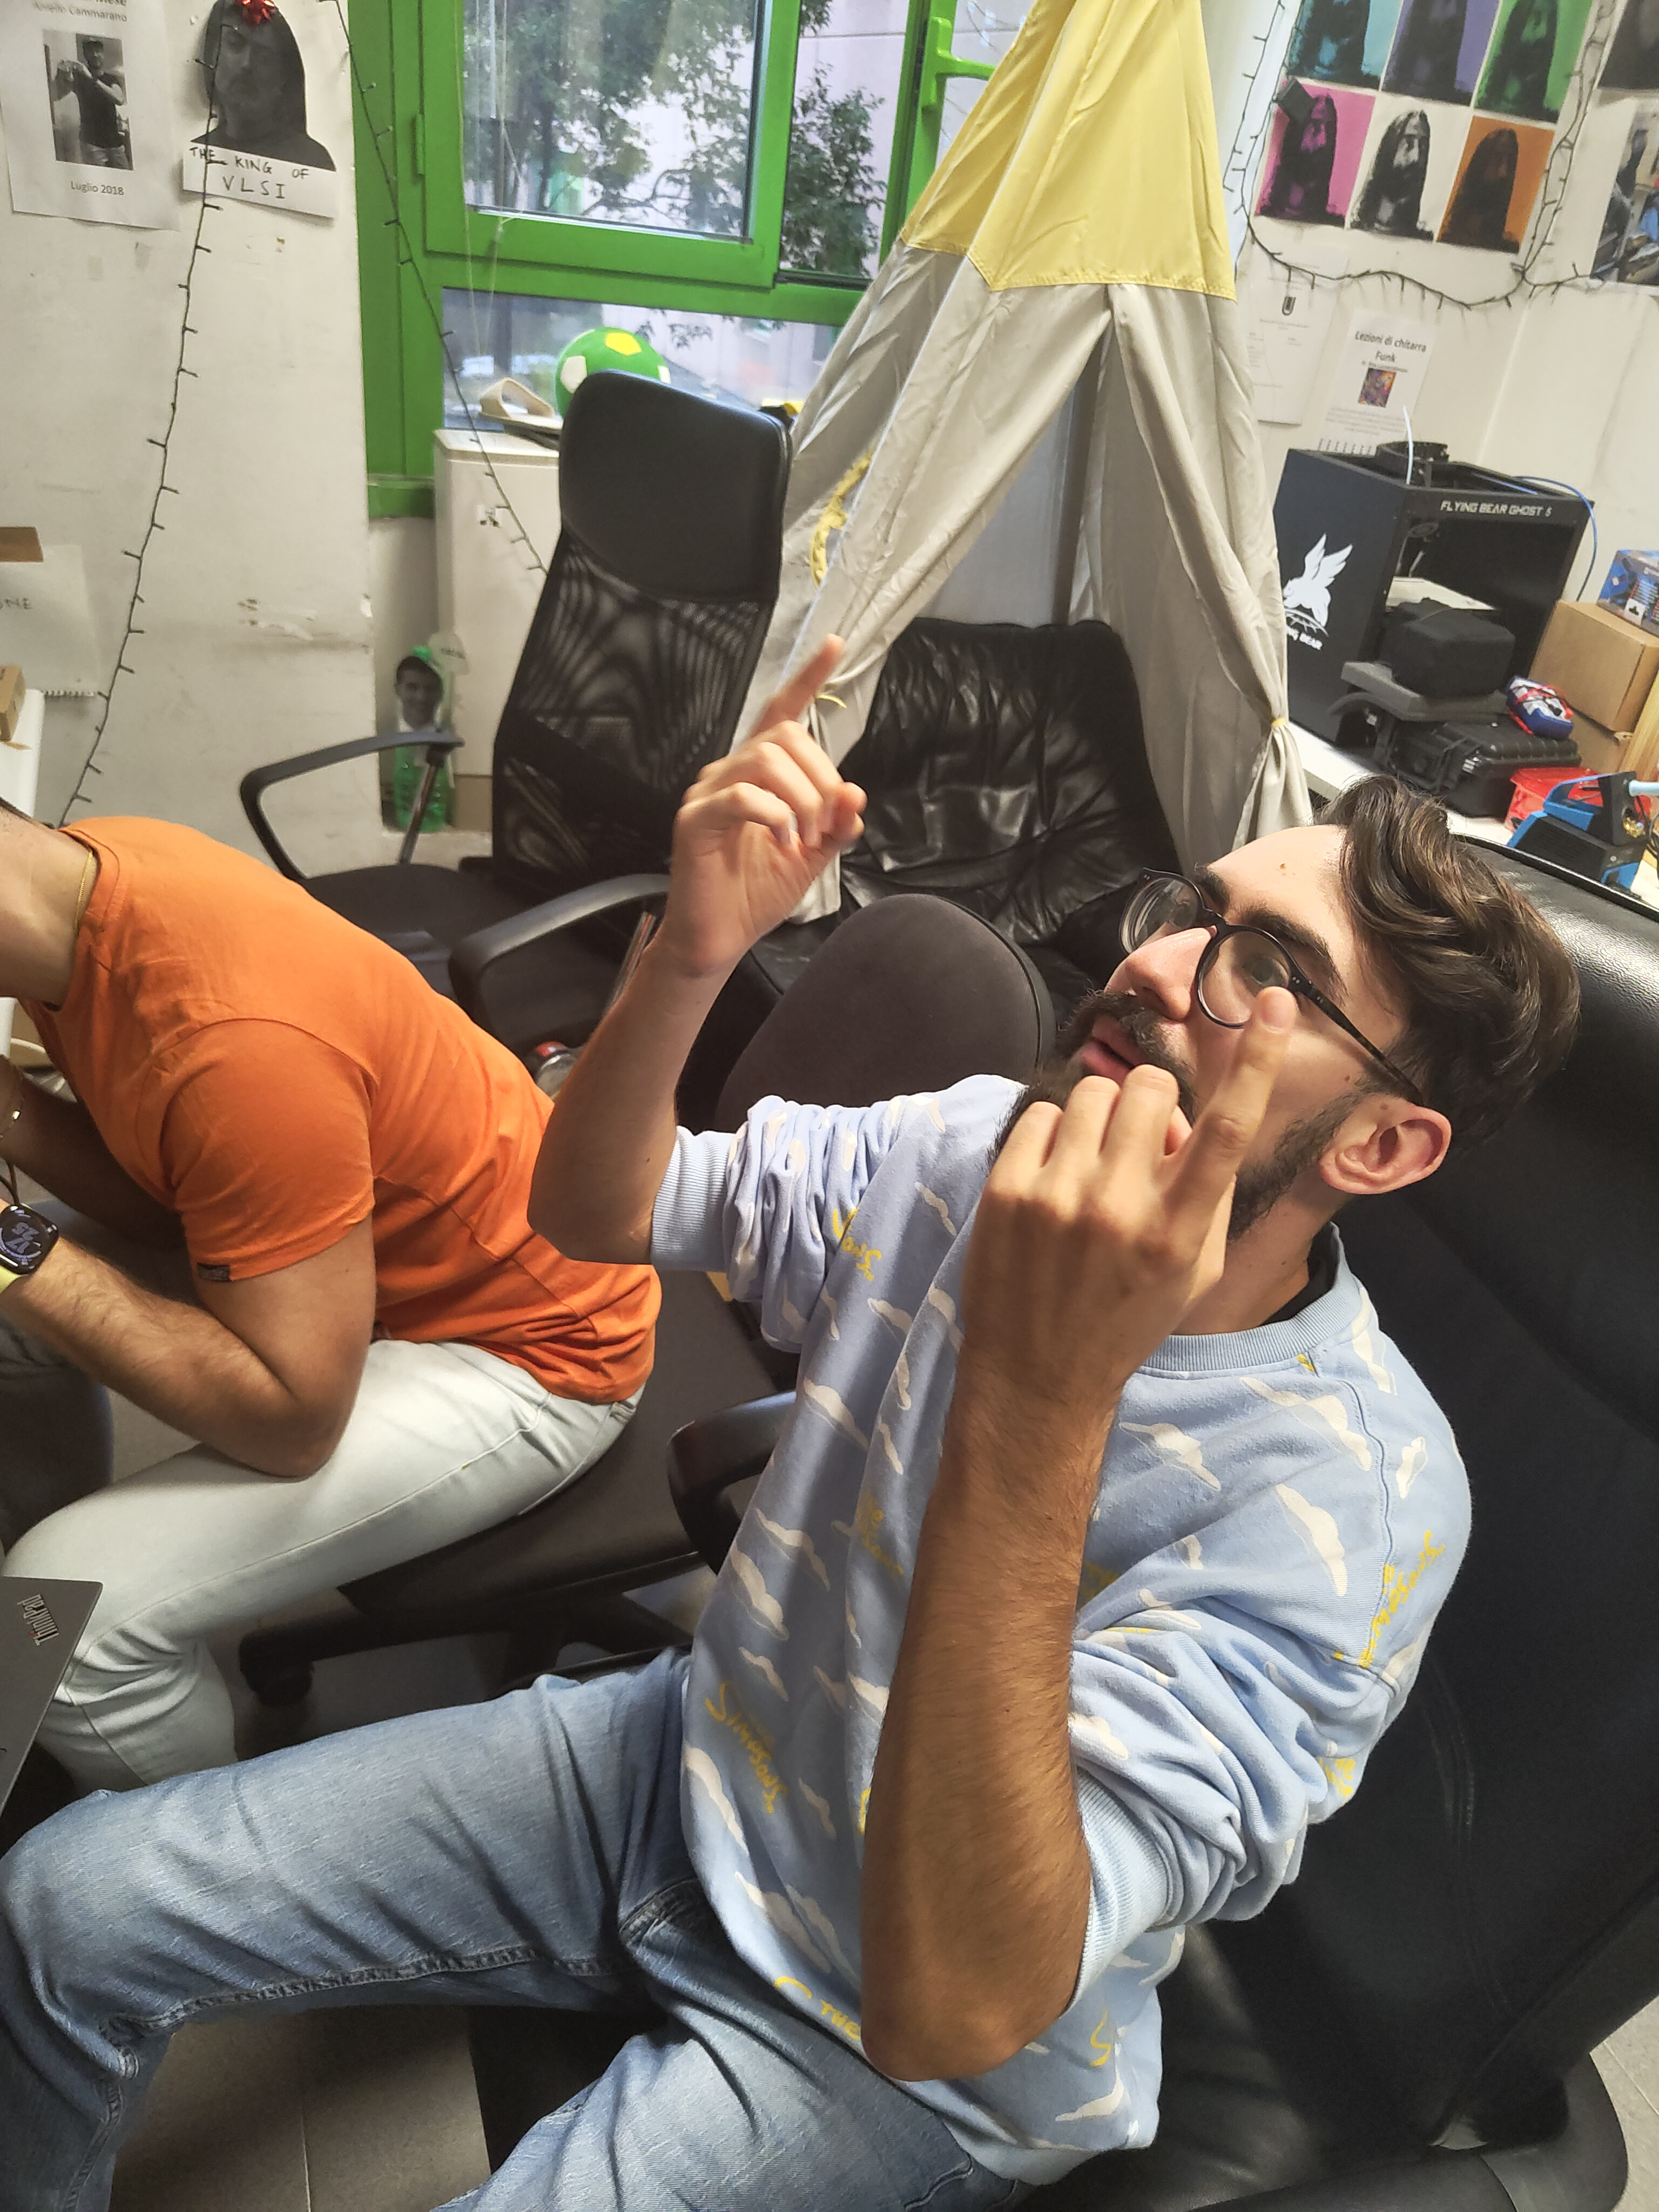
\includegraphics[width=0.3\linewidth]{assets/eureka_1.jpg}}\hfill
				\subfloat{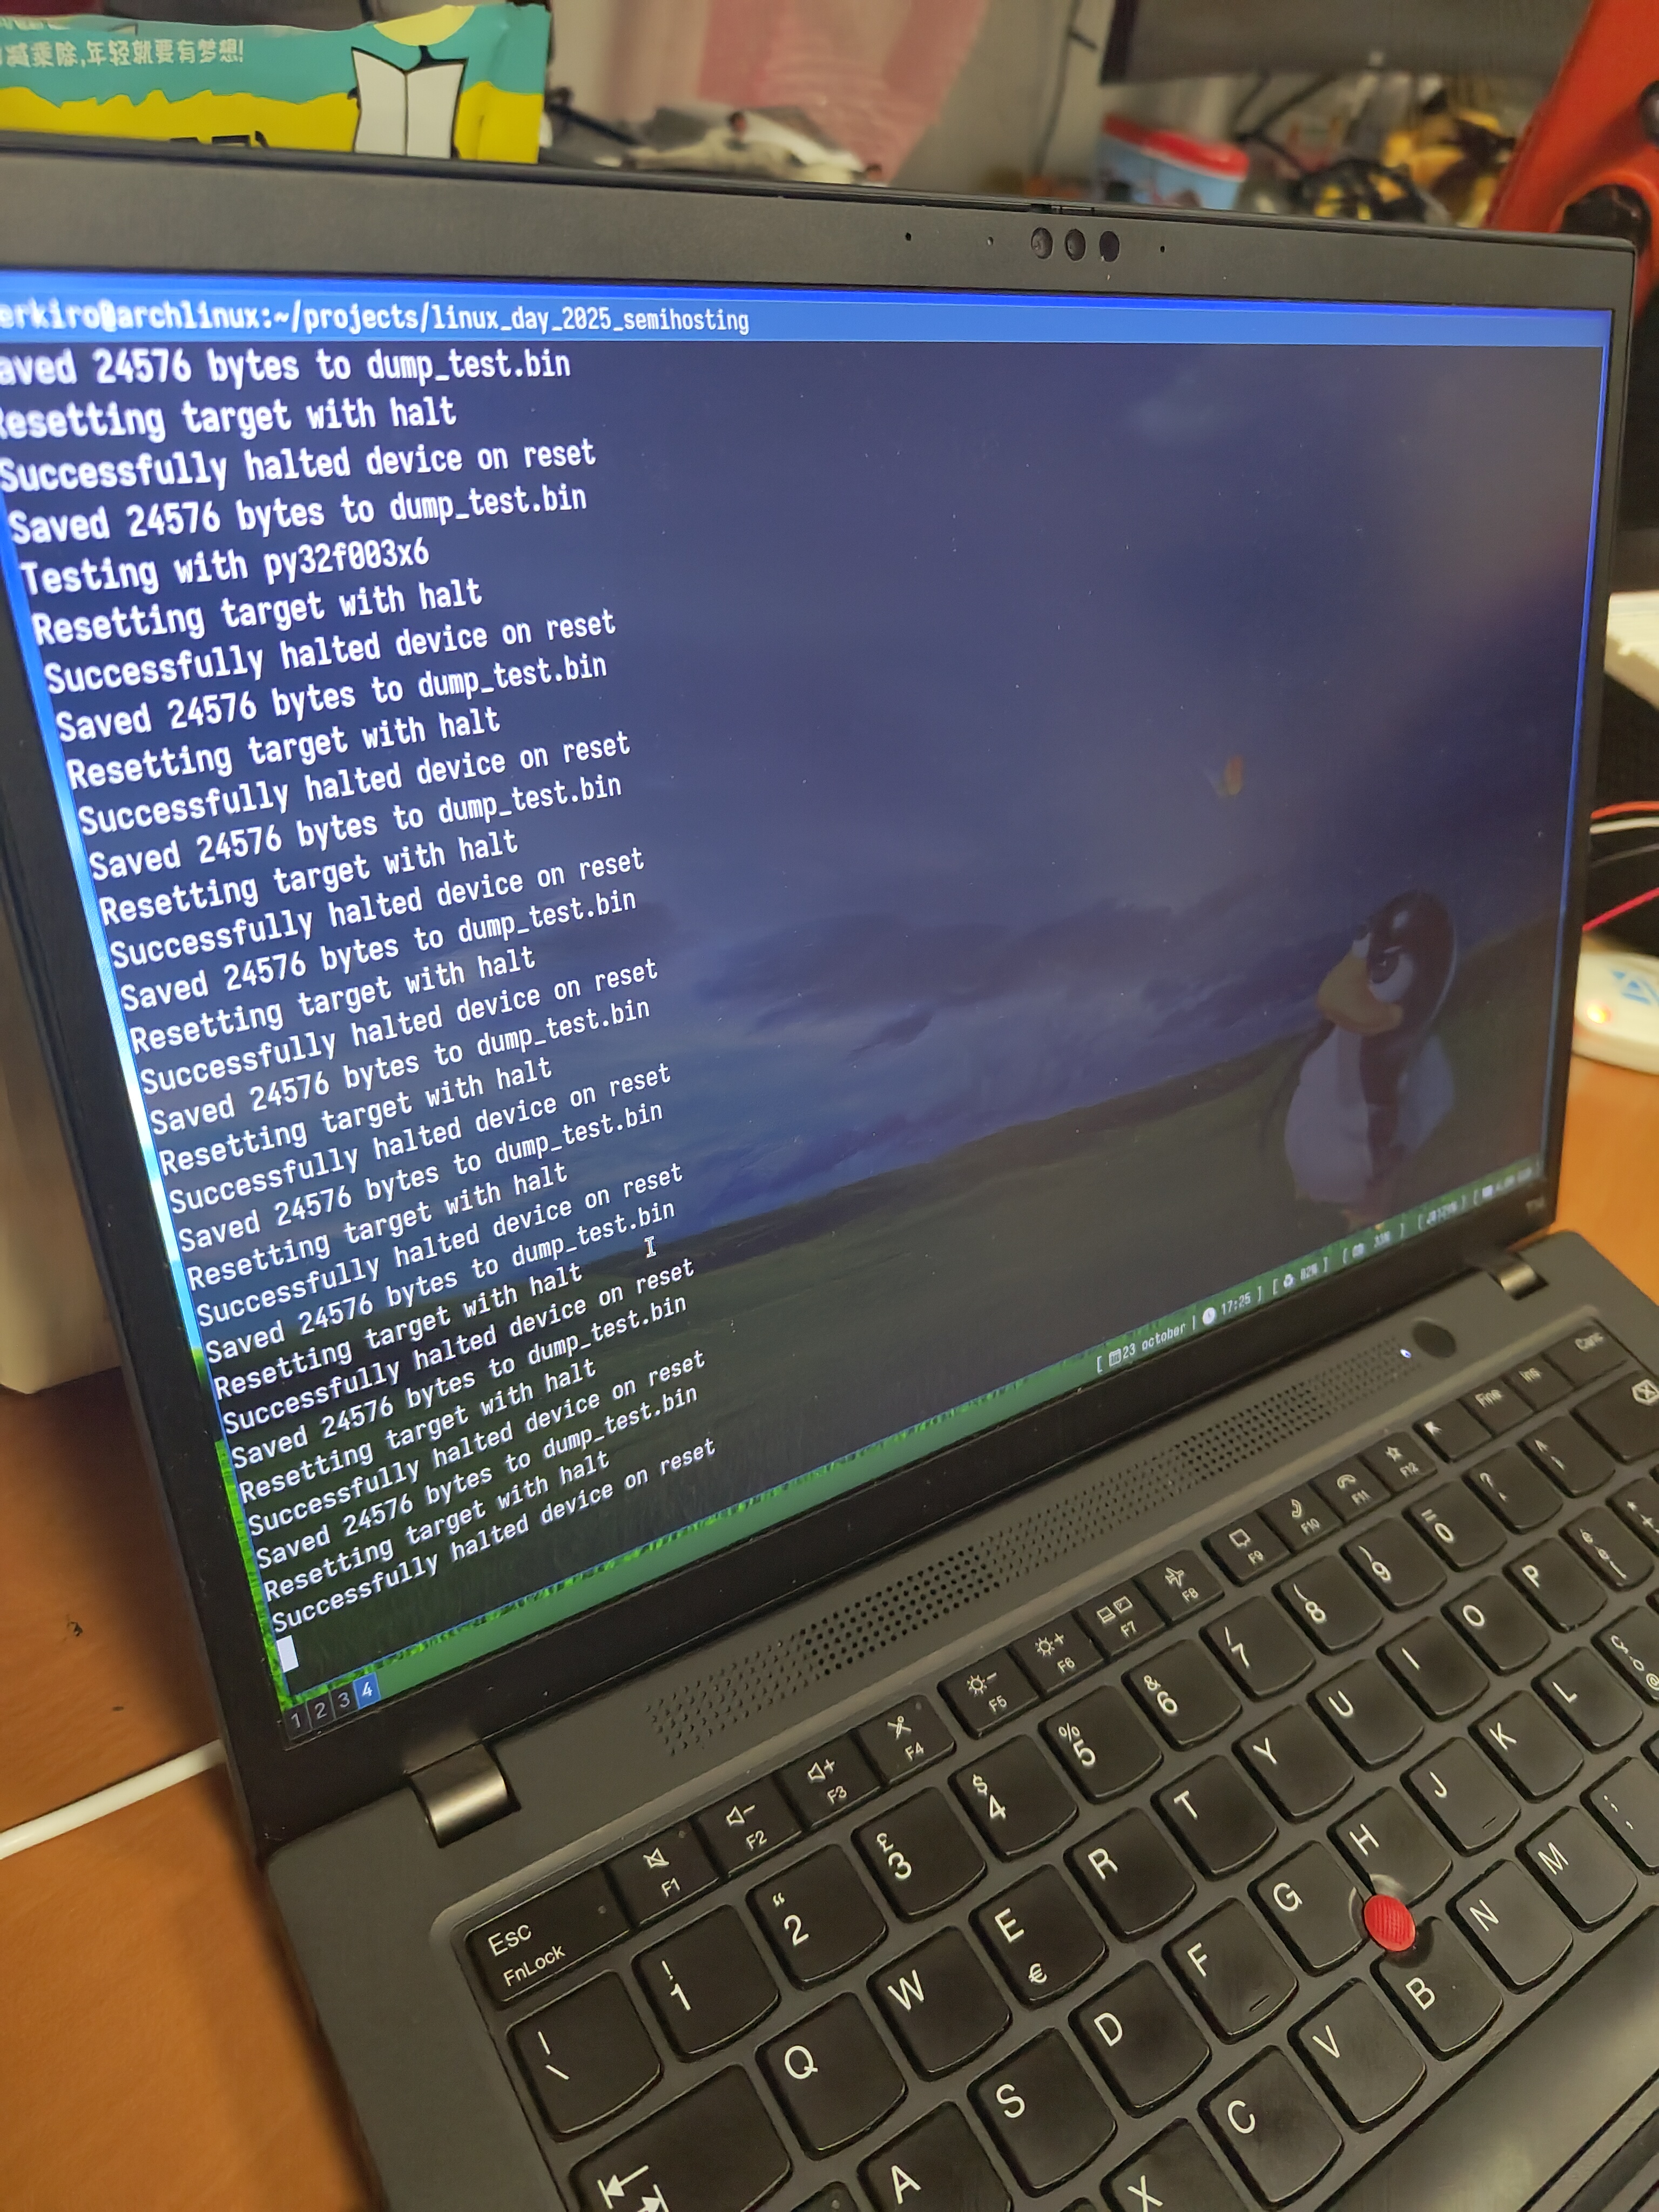
\includegraphics[width=0.3\linewidth]{assets/eureka_2.jpg}}\hfill
  				\subfloat{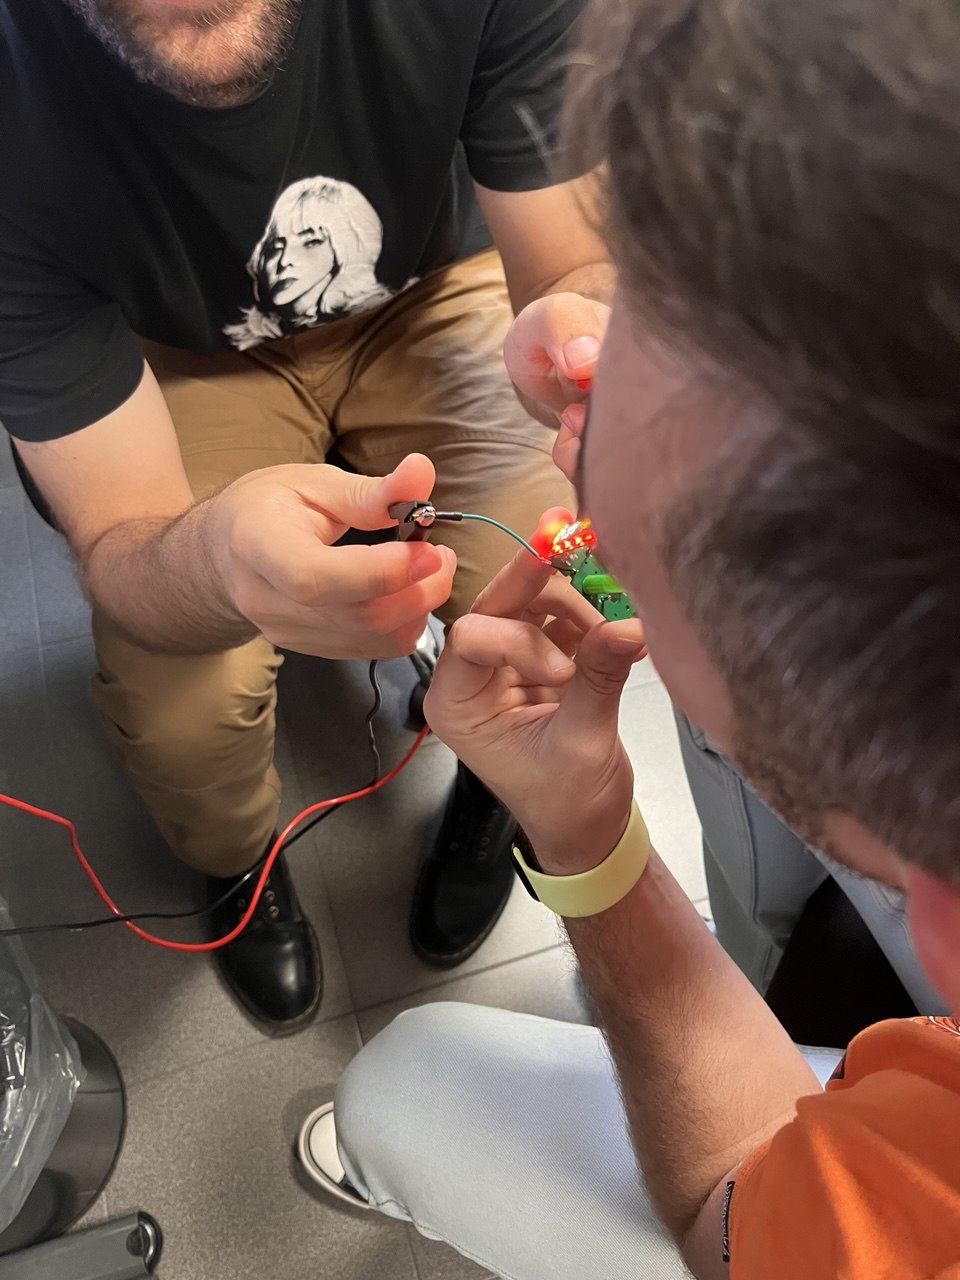
\includegraphics[width=0.3\linewidth]{assets/soffio_1.jpg}}\hfill%
			\end{figure}
		\end{frame}
	\end{NoHyper}

   \begin{NoHyper}
	   \begin{frame}{Memory layout}
		   Memory layout for our Puya chip
		   \begin{figure}
			   \centering
			   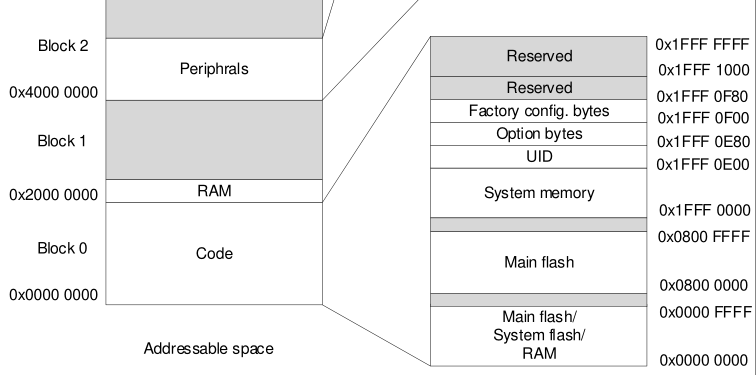
\includegraphics[width=.95\textwidth]{assets/mem_layout}
		   \end{figure}
		\end{frame}
	\end{NoHyper}

   \begin{NoHyper}
	   \begin{frame}{Firmware compilation}
		   \begin{itemize}
			   \item The fun part ended, now it was time for the software upload
			   \item \textbf{Goal:} upload a firmware that would output "Hello World!" on our terminal upon connecting through SWD
			   \item Software needed (at a high level)
				   \begin{itemize}
			   			\item Debian 11 OS
			   			\item \texttt{arm-none-eabi} toolchain for cross compilation
			   			\item \texttt{pyocd} to interact with the hardware
				   \end{itemize}
		   \end{itemize}
		\end{frame}
	\end{NoHyper}

   \begin{NoHyper}
	   \begin{frame}{Firmware compilation - env setup}
		   \begin{itemize}
			   \item[\$] \texttt{sudo apt install gcc-arm-none-eabi} 
			   \item[\$] \texttt{git clone https://github.com/BogdanTheGeek/semihost-ip.git}
			   \item[\$] \texttt{cd semihost-ip}
			   \item[\$] \texttt{python3 -m venv pyocd}
			   \item[\$] \texttt{source pyocd/bin/activate}
			   \item[\$] \texttt{python3 -mpip install -U pyocd}
		   \end{itemize}
		\end{frame}
	\end{NoHyper}

   \begin{NoHyper}
	   \begin{frame}{Firmware compilation - dump existing firmware}
		\begin{minipage}[b]{.5\textwidth}
			\begin{itemize}
				\item [\$] \texttt{pyocd cmd -t py32f030x -f 1m -c reset halt -c savemem 0x08000000 0x6000 bin\_dump.bin}
			\end{itemize}
		\end{minipage}%
		\begin{minipage}[b]{.5\textwidth}
			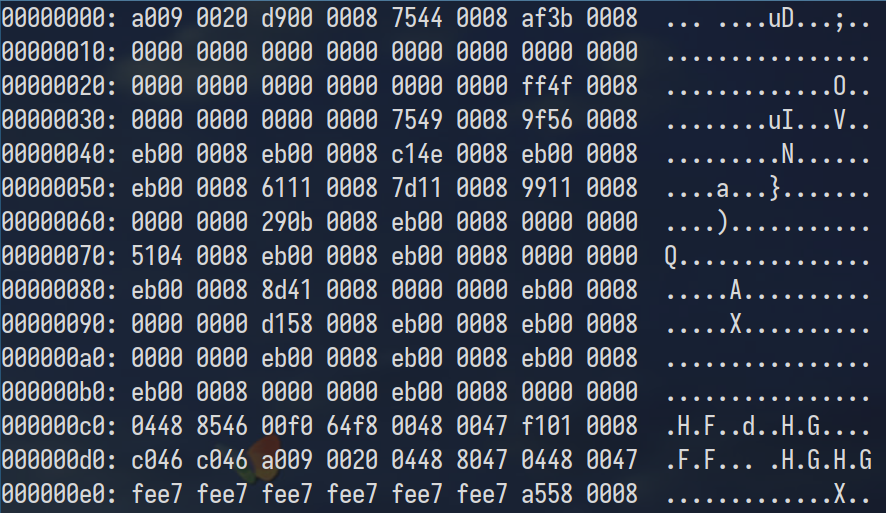
\includegraphics[width=\textwidth]{assets/hexdump}
		\end{minipage}%
		\end{frame}
	\end{NoHyper}

   \begin{NoHyper}
	   \begin{frame}{Firmware compilation - new firmware}
		   \lstinputlisting[language=C]{code/hello.c}
		\end{frame}
	\end{NoHyper}

   \begin{NoHyper}
	   \begin{frame}{Firmware compilation - making and flashing}
		   \begin{itemize}
			   \item[\$] \texttt{cd semihost-ip}
			   \item[\$] \texttt{make all}
			   \item[\$] \texttt{pyocd load -t py32f030x6 -f 1m bin/firmware.bin}
		   \end{itemize}
		\end{frame}
	\end{NoHyper}

   \begin{NoHyper}
	   \begin{frame}{Firmware compilation - Hello, eCig!}
			Run the following commands in separate terminals (behold the order!)
			\begin{itemize}
				\item [\$] \texttt{pyocd gdb -S -O semihost\_console\_type=telnet -t py32f030x6 -f 24m --elf firmware.elf} 
				\item [\$] \texttt{arm-none-eabi-gdb -ex "target extended-remote localhost:3333" -ex "monitor arm semihosting enable"}
				\item [\$] \texttt{telnet localhost 4444} 
			\end{itemize}
		\end{frame}
	\end{NoHyper}

   \begin{NoHyper}
	   \begin{frame}{Firmware compilation - Hello, eCig! (or maybe not)}
			\begin{itemize}
				\item Still, we were facing an issue, since from \texttt{gdb} we saw PC struck on an infinite loop on \texttt{ADC\_COMP\_IRQHandler}
				\item At this point we were running out of time, so the turnaround was to force GDB to go at the start of main
				\item [\$] \texttt{set \$pc = 0x08001d16}
			\end{itemize}
		\end{frame}
	\end{NoHyper}

   \begin{NoHyper}
	   \begin{frame}{Finally, at 2 a.m in Cave (RM, Italy)...}
		   \begin{figure}
			   \centering
			   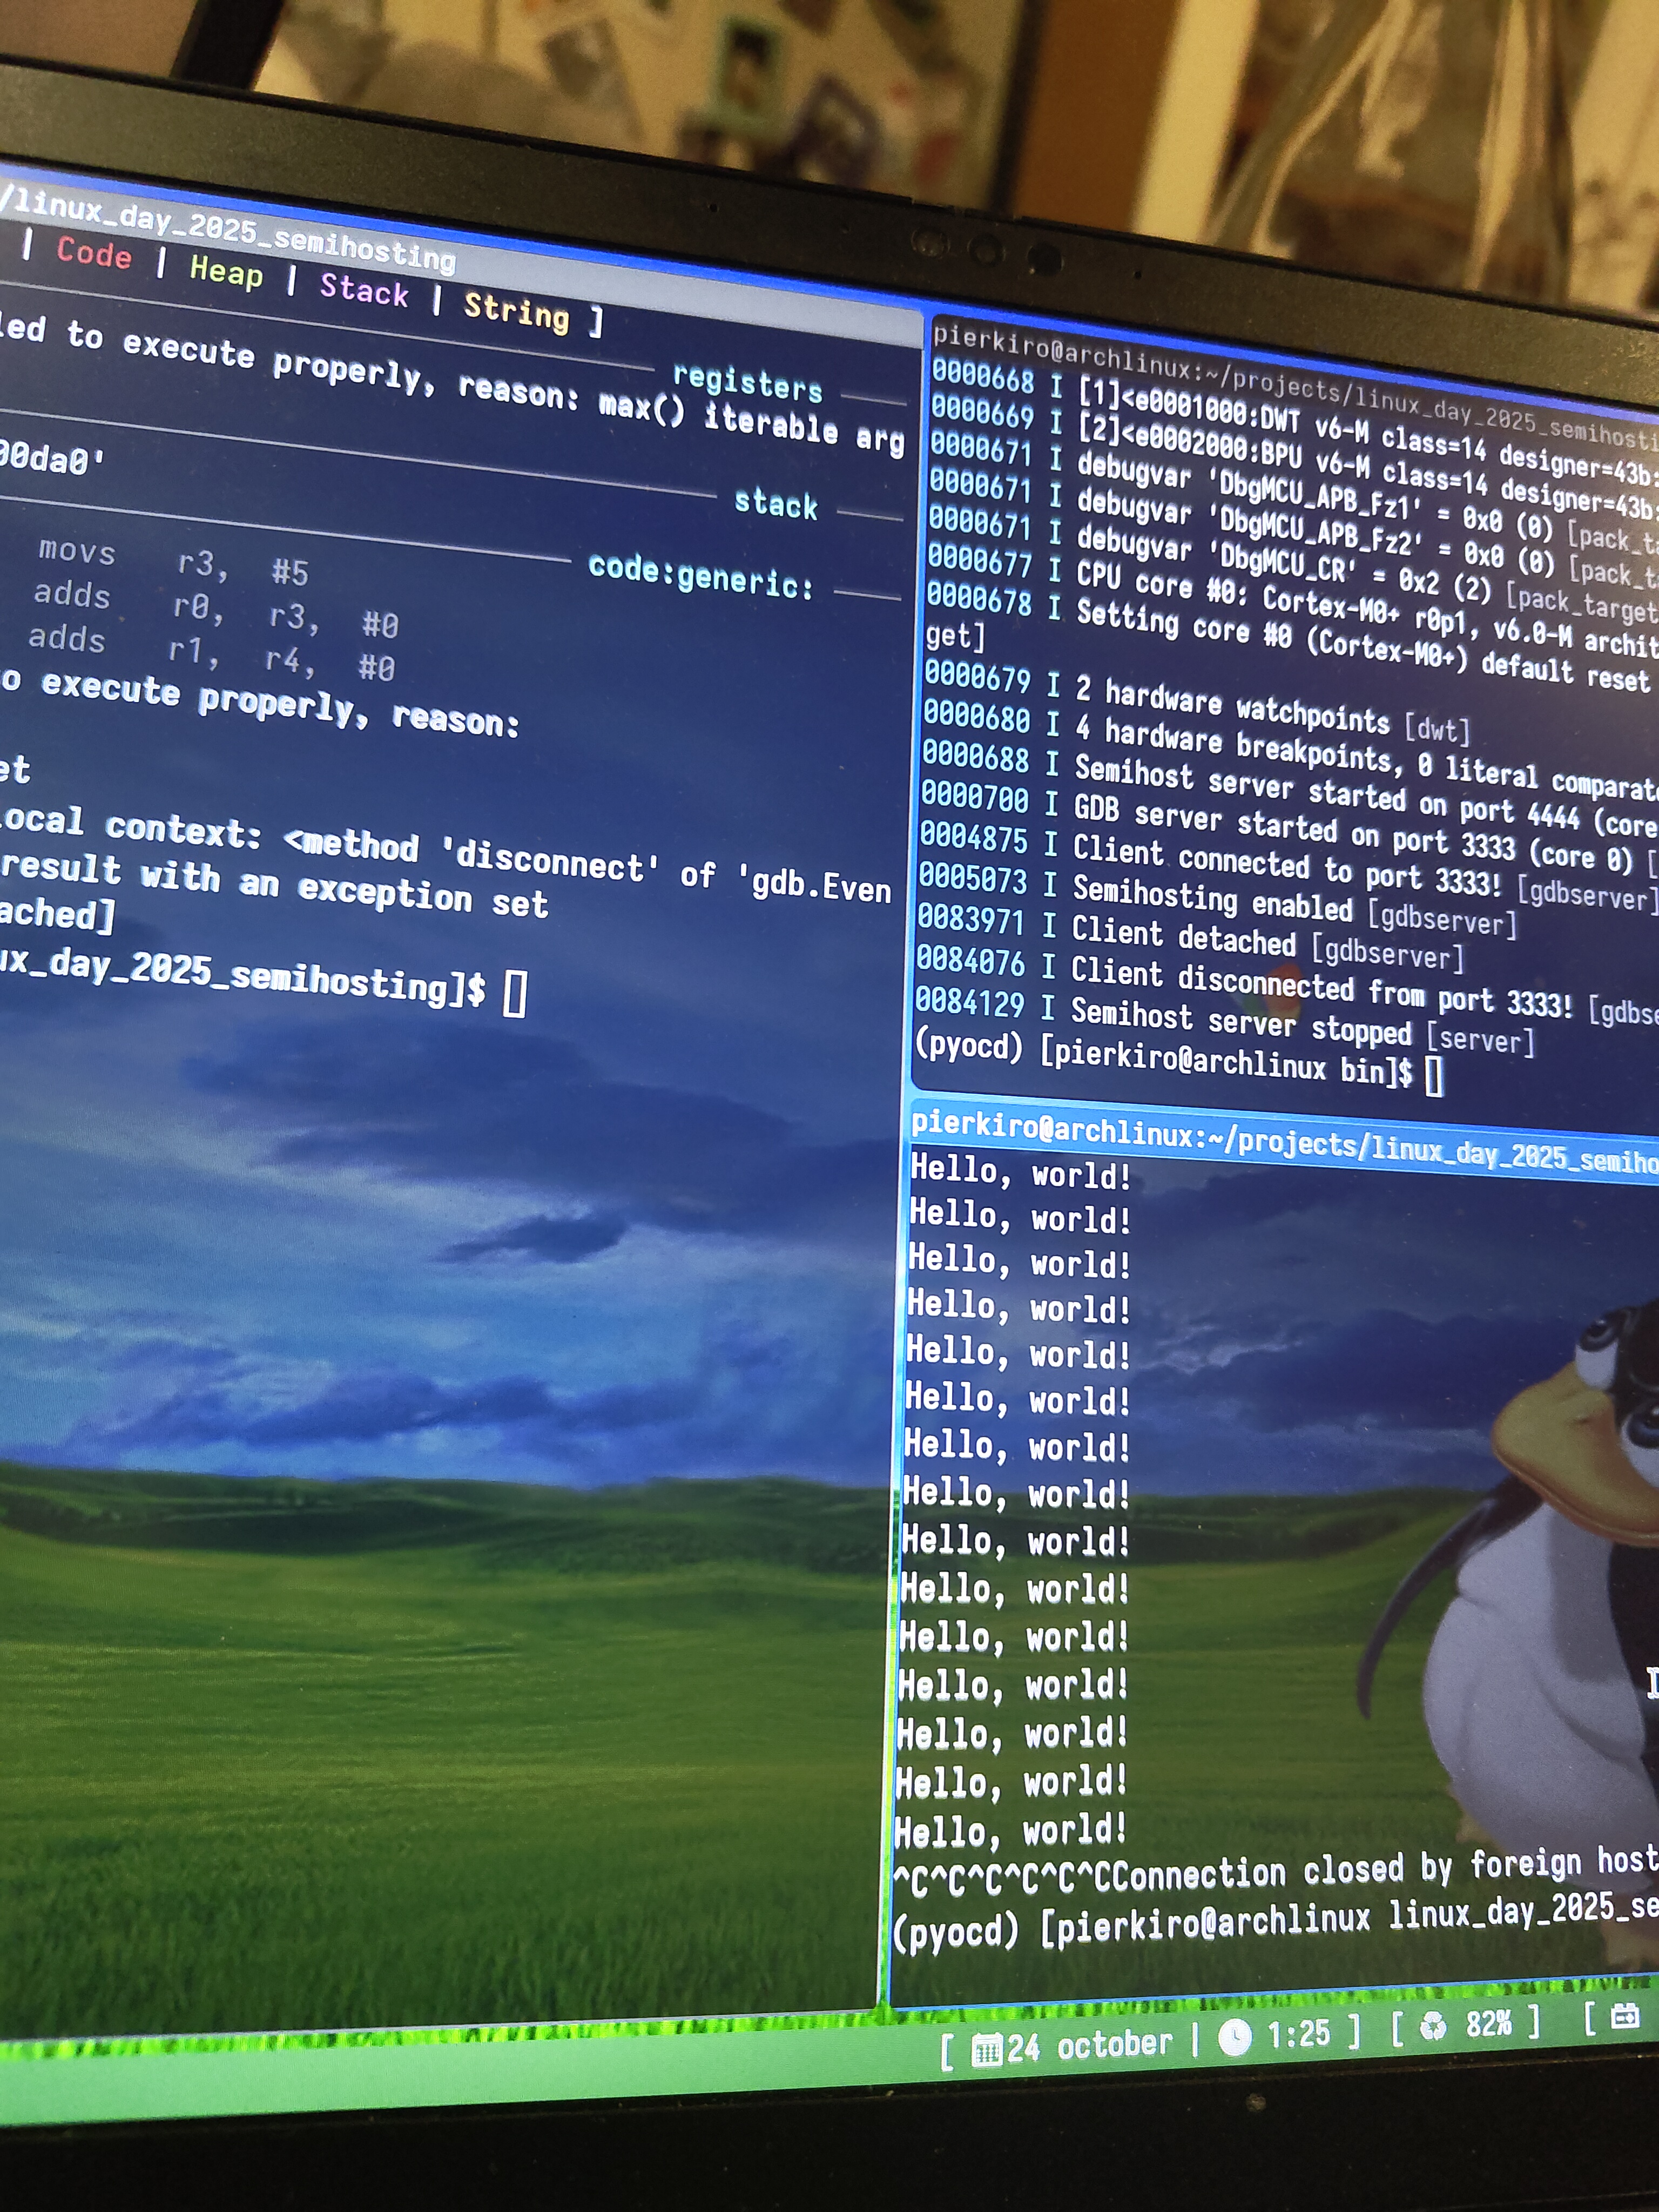
\includegraphics[width=.45\textwidth]{assets/final}
		   \end{figure}
		\end{frame}
	\end{NoHyper}


   \begin{NoHyper}
	   \begin{frame}{Thank you very much!}
		   \begin{figure}
			   \centering
			   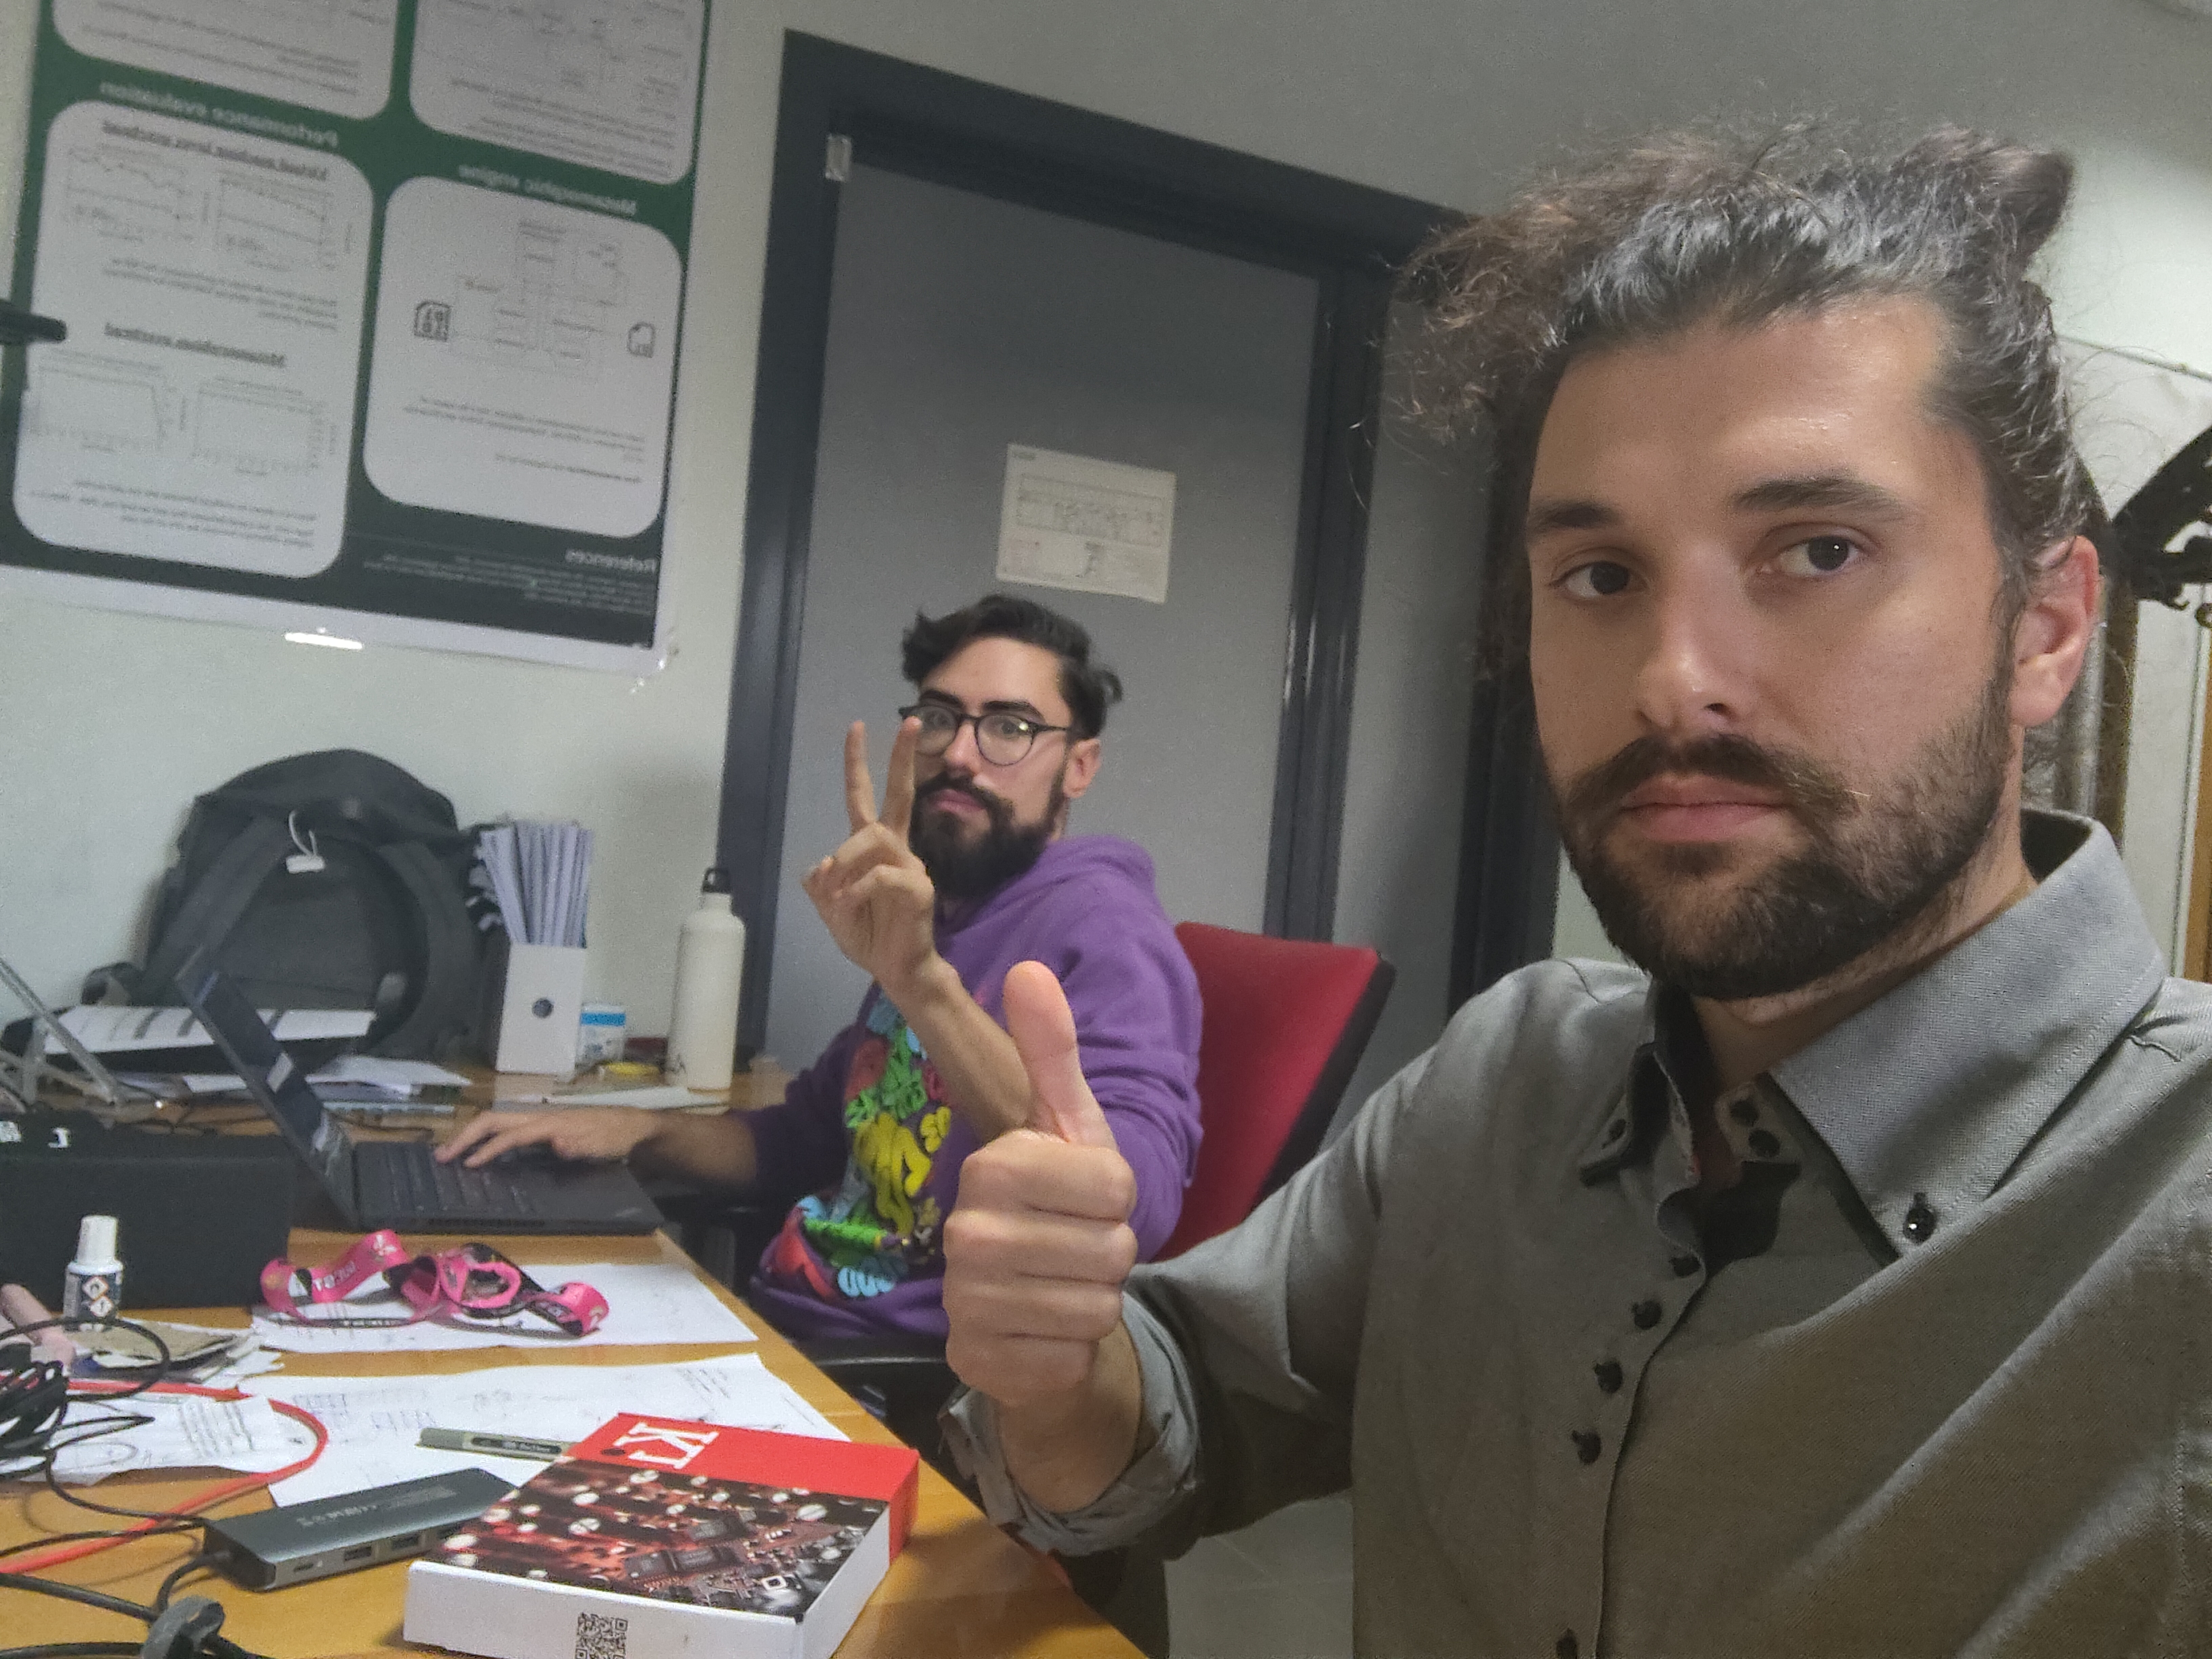
\includegraphics[width=.8\textwidth]{assets/slide_finale}
		   \end{figure}
		\end{frame}
	\end{NoHyper}

	\begin{frame}[allowframebreaks]{References}
		\begin{itemize}
			\item \href{https://github.com/pyocd/pyOCD/blob/main/docs/semihosting.md}{semihosting guide}
			\item \href{https://interrupt.memfault.com/blog/a-deep-dive-into-arm-cortex-m-debug-interfaces}{semihosting guide pt 2}
			\item \href{https://embeddedinventor.com/a-complete-beginners-guide-to-the-gnu-arm-toolchain-part-1/}{Beginner guide to GNU arm}
			\item \href{https://github.com/BogdanTheGeek/semihost-ip/tree/main}{semihost ip repo}
			\item \href{https://developer.arm.com/downloads/-/arm-gnu-toolchain-downloads}{arm-gnu-toolchain-downloads}
		\end{itemize}
	\end{frame}
\end{document}
